\chapter{Resultados y Análisis}

Una vez realizados los experimentos con el algoritmo de agrupamiento X-Means, se presentan los resultados en diferentes figuras y tablas. Primero se encuentran los resultados conseguidos al ejecutar el algoritmo con los atributos de las tablas \ref{tab:atributos_establecimientos} y \ref{tab:atributos_matriculas}, para ver cuales atributos son los mas importantes. Luego se presentan los resultados al comparar el mejor resultado de la etapa anterior con el resultado que se obtiene al agregarle las variables de relación establecimiento-matrícula.

\section{Resultados obtenidos}

La tabla \ref{tab:cl_estab} muestra los resultados al ejecutar X-Means sobre la base de datos de establecimientos en 3 diferentes ocasiones, diferenciándose por la cantidad de atributos que se utilizan. Una con todos los atributos, una con los de importancia alta y media, y finalmente una solo con los atributos de importancia alta.

Las siglas de los clústers de establecimientos sin considerar los atributos de relación establecimientos-matrícula (tablas \ref{tab:cl_estab}, \ref{tab:cl_atr_estab} y \ref{tab:cl_depe_estab}) corresponden a:

\begin{itemize}
    \item BCBM: Bajo Costo Baja Matricula (menor a 390 alumnos).
    \item BCAM: Bajo Costo Alta Matricula (sobre 700 alumnos).
    \item MCAM: Medio Costo Alta Matricula (sobre 700 alumnos).
    \item ACMM: Alto Costo Media Matrícula (entre 391 y 700 alumnos).
\end{itemize}

\begin{table}[H]
\centering
\caption{Clústers de establecimientos variando la cantidad de atributos (por grupos de importancia).}
\label{tab:cl_estab}
\begin{tabular}{|c|c|c|c|c|}
\hline
\textbf{Atributos} & \textbf{BCBM} & \textbf{BCAM} & \textbf{MCAM} & \textbf{ACMM}   \\ \hline
Todos & 959 & 826 & 247 & 36 \\ \hline
Alta + Media & 959 & 540 & 311 & 258 \\ \hline
Alta & 977 & 524 & 308 & 259\\ \hline
\end{tabular}
\end{table}

La tabla \ref{tab:cl_atr_estab} muestra los resultados obtenidos al ejecutar X-Means en los atributos de la base de datos de establecimientos (tabla \ref{tab:atributos_establecimientos}) con importancia alta.

\begin{table}[H]
\centering
\caption{Comparativa de clústers de establecimientos por atributo.}
\label{tab:cl_atr_estab}
\resizebox{\textwidth}{!}{\begin{tabular}{|l|l|l|l|l|}
\hline
& \textbf{BCBM} & \textbf{BCAM} & \textbf{MCAM} & \textbf{ACMM} \\ \hline
\textbf{Dependencia}                    & P.Subvencionado / Municipal & \begin{tabular}[c]{@{}l@{}}P. Subvencionado / Municipal / \\ Corp. Adm. Deleagada\end{tabular} & P. Subvencionado   & P. Pagado        \\ \hline
\textbf{Educación}               & Básica / Media              & Media / Completa                                                                               & Media / Completa   & Completa         \\ \hline
\textbf{Matrícula}               & Gratuita / Menor a \$25.000 & Gratuita / Menor a \$25.000                                                                    & Menor a \$10.000   & Mayor a \$50.000 \\ \hline
\textbf{Mensualidad}             & Gratuita / Menor a \$25.000 & Gratuita / Menor a \$25.000                                                                    & $25.000 - $100.000 & Mayor a \$50.000 \\ \hline
\textbf{Convenio SEP}            & Si                          & Si                                                                                             & No                 & No               \\ \hline
\textbf{Prom. matrículas}        & 383                         & 781                                                                                            & 905                & 686              \\ \hline
\textbf{Prom. alumnos por curso} & 26                          & 30                                                                                             & 32                 & 21               \\ \hline
\textbf{Prom. de becas}          & 19                          & 59                                                                                             & 91                 & 8                \\ \hline
\end{tabular}}
\end{table}

\begin{table}[H]
\centering
\caption{Clústers de establecimientos (tabla \ref{tab:cl_atr_estab}) según su dependencia.}
\label{tab:cl_depe_estab}
\begin{tabular}{|c|c|c|c|c|}
\hline
\textbf{Clúster} & \textbf{Municipal} & \textbf{P. Subvencionado} & \textbf{P. Pagado} & \textbf{Corp. Admin. Del.}   \\ \hline
BCBM & 485 & 491 & 1 & 0 \\ \hline
BCAM & 173 & 318 & 0 & 33 \\ \hline
MCAM & 3 & 303 & 2 & 0 \\ \hline
ACMM & 0 & 1 & 258 & 0 \\ \hline
\end{tabular}
\end{table}

En la tabla \ref{tab:cl_atr_estab_rel} se encuentran los resultados que se obtuvieron al ejecutar el algoritmo de agrupamiento en la base de datos conformada por los atributos de importancia alta de la tabla \ref{tab:atributos_establecimientos} y los atributos de relación establecimiento-matrícula de la tabla \ref{tab:atributos_relacion_establecimientos}.

Las siglas utilizadas para los clústers de establecimientos considerando los atributos de relación establecimientos-matrícula (tablas \ref{tab:cl_atr_estab_rel}, \ref{tab:cl_depe_estab_rel} y \ref{tab:cl_estab_sobre_edad}) corresponden a:
\begin{itemize}
    \item BCBMCD: Bajo Costo Baja Matricula (menor a 390 alumnos) Corta Distancia (menor a 4 km).
    \item BCAMMD: Bajo Costo Alta Matricula (sobre 700 alumnos) Media Distancia (entre 4 y 8 km).
    \item MCAMMD: Medio Costo Alta Matricula (sobre 700 alumnos) Media Distancia (entre 4 y 8 km).
    \item ACMMLD: Alto Costo Media Matrícula (entre 391 y 700 alumnos) Larga Distancia (sobre 8 km).
\end{itemize}

\begin{table}[H]
\centering
\caption{Comparativa de clústers de establecimientos por atributo, incluyendo los de relación establecimiento-matrícula.}
\label{tab:cl_atr_estab_rel}
\resizebox{\textwidth}{!}{\begin{tabular}{|l|l|l|l|l|}
\hline
& \textbf{BCBMPD} & \textbf{BCAMMD} & \textbf{MCAMMD} & \textbf{ACMMLD} \\ \hline
\textbf{Dependencia}                                                                  & P. Subvencionado / Municipal & \begin{tabular}[c]{@{}l@{}}P. Subvencionados / Municipales /\\ Corp. Adm. Delegada\end{tabular} & P. Subvencionado   & P. Pagado        \\ \hline
\textbf{Educación}                                                                    & Básica                       & Media / Completa                                                                                & Media / Completa   & Completa         \\ \hline
\textbf{Matrícula}                                                                    & Gratuita                     & Gratuita / Menor a \$25.000                                                                     & Menor a \$10.000   & Mayor a \$50.000 \\ \hline
\textbf{Mensualidad}                                                                  & Gratuita / Menor a \$25.000  & Gratuita / Menor a \$25.000                                                                     & $25.000 - $100.000 & Mayor a \$50.000 \\ \hline
\textbf{Convenio SEP}                                                                 & Si                           & Si                                                                                              & No                 & No               \\ \hline
\textbf{Prom. matrículas}                                                             & 383                          & 781                                                                                             & 895                & 686              \\ \hline
\textbf{Prom. alumnos por curso}                                                      & 26                           & 30                                                                                              & 32                 & 21               \\ \hline
\textbf{Prom. de becas}                                                               & 19                           & 58                                                                                              & 91                 & 8                \\ \hline
\textbf{IDE}                                                                          & 0,5 - 1                      & -0,5 - 0                                                                                        & 0 - 1,5            & 1 - 1,5          \\ \hline
\begin{tabular}[c]{@{}l@{}}\textbf{Distancia}\\ \textbf{Establecimiento - Hogar}\end{tabular} & 2,960 km                     & 5,204 km                                                                                        & 5,207 km           & 9,761            \\ \hline
\textbf{Sobre edad promedio}                                                                   & 0,524                        & 0,488                                                                                           & 0,297              & 0,488            \\ \hline
\end{tabular}}
\end{table}

\begin{table}[H]
\centering
\caption{Clústers de establecimientos (tabla \ref{tab:cl_atr_estab_rel}) según su dependencia.}
\label{tab:cl_depe_estab_rel}
\begin{tabular}{|c|c|c|c|c|}
\hline
\textbf{Clúster} & \textbf{Municipal} & \textbf{P. Subvencionado} & \textbf{P. Pagado} & \textbf{Corp. Admin. Del.}   \\ \hline
BCBMPD & 485 & 489 & 1 & 0 \\ \hline
BCAMMD & 173 & 307 & 0 & 33 \\ \hline
MCAMMD & 3 & 316 & 2 & 0 \\ \hline
ACMMLD & 0 & 1 & 258 & 0 \\ \hline
\end{tabular}
\end{table}

\begin{table}[H]
\centering
\caption{Detalle de la sobre edad en los clústers de establecimientos. }
\label{tab:cl_estab_sobre_edad}
\begin{tabular}{|l|c|c|c|c|c|}
\hline
                & \textbf{\% del total} & \textbf{\% 1 año\footnotemark} & \textbf{\% 2 años\footnotemark[\value{footnote}]\footnotemark[\value{footnote}]} & \textbf{\% 3 años\footnotemark[\value{footnote}]} & \textbf{\% 4 años\footnotemark[\value{footnote}]} \\ \hline
\textbf{BCBMPD} & 31                    & 74,8              & 18,9               & 5,2                & 1,1                \\ \hline
\textbf{BCAMMD} & 32,9                  & 75,1              & 20,5               & 3,9                & 0,5                \\ \hline
\textbf{MCAMMD} & 24                    & 85,3              & 13                 & 1,6                & 0,1                \\ \hline
\textbf{ACMMLD} & 38,1                  & 94,9              & 4,6                & 0,4                & 0,1                \\ \hline
\end{tabular}
\end{table}

\footnotetext{Porcentajes en base al total de alumnos con sobre edad mayor o igual a 1.}

Las siguientes tablas, y de manera similar a lo descrito anteriormente para los establecimientos, muestran los resultados obtenidos usando los datos de las matrículas. En la tabla \ref{tab:cl_mat} se muestran los resultados con los datos de la tabla \ref{tab:atributos_matriculas} en 3 diferentes versiones, según la importancia del atributo. La primera con todos los atributos, luego solo con los de alta y media, y finalmente solo los de alta importancia.

Las siglas utilizadas para los clústers de matrículas sin atributos de relación (tablas \ref{tab:cl_mat}, \ref{tab:cl_atr_mat} y \ref{tab:cl_mat_sobre_edad}) corresponden a:

\begin{itemize}
    \item MCB: Mujeres Con Beneficio.
    \item HCB: Hombres Con Beneficio.
    \item MSB: Mujeres Sin Beneficio.
    \item HSB: Hombres Sin Beneficio.
\end{itemize}

\begin{table}[H]
\centering
\caption{Clústers de matrículas variando la cantidad de atributos (por grupos de importancia).}
\label{tab:cl_mat}
\begin{tabular}{|c|c|c|c|c|}
\hline
\textbf{Atributos} & \textbf{MCB} & \textbf{HCB} & \textbf{MSB} & \textbf{HSB}   \\ \hline
Todos & 551932 & 442048 & 40803 & 13585 \\ \hline
Alta + Media & 551932 & 442048 & 34088 & 20300 \\ \hline
Alta & 286089 & 300007 & 230486 & 231786 \\ \hline
\end{tabular}
\end{table}

En las tablas \ref{tab:cl_atr_mat} y \ref{tab:cl_atr_mat_rel} se muestran primero los resultados obtenidos al utilizar los atributos de alta importancia de la tabla \ref{tab:atributos_matriculas} y luego los que se obtienen al incluir los atributos de relación de la tabla \ref{tab:atributos_relacion_matriculas}.

\begin{table}[H]
\centering
\caption{Comparativa de clústers de matrículas por atributo.}
\label{tab:cl_atr_mat}
\resizebox{\textwidth}{!}{\begin{tabular}{|l|l|l|l|l|}
\hline
& \textbf{MCB} & \textbf{HCB} & \textbf{MSB} & \textbf{HSB} \\ \hline
\textbf{Género}           & Femenino                                                                                                         & Masculino                                                                                                        & Femenino & Masculino \\ \hline
\textbf{Beneficiario SEP} & Si                                                                                                               & Si                                                                                                               & No       & No        \\ \hline
\textbf{Criterio SEP}     & \begin{tabular}[c]{@{}l@{}}Pertenece a Chile solidario / \\ Puntaje de ficha de protección\\ social\end{tabular} & \begin{tabular}[c]{@{}l@{}}Pertenece a Chile solidario / \\ Puntaje de ficha de protección\\ social\end{tabular} &          &           \\ \hline
\textbf{Sobre edad}       & 0,364                                                                                                            & 0,488                                                                                                            & 0,284    & 0,365     \\ \hline
\end{tabular}}
\end{table}


\begin{table}[H]
\centering
\caption{Detalle de la sobre edad en los clústers de matrículas.}
\label{tab:cl_mat_sobre_edad}
\begin{tabular}{|l|c|c|c|c|c|}
\hline
             & \textbf{\% del total} & \textbf{\% 1 año\footnotemark} & \textbf{\% 2 años\footnotemark[\value{footnote}]} & \textbf{\% 3 años\footnotemark[\value{footnote}]} & \textbf{\% 4 años\footnotemark[\value{footnote}]} \\ \hline
\textbf{MCB} & 28,5                  & 76,9              & 18,5               & 4                  & 0,6                \\ \hline
\textbf{HCB} & 36,4                  & 72,5              & 21,5               & 5,1                & 0,9                \\ \hline
\textbf{MSB} & 25,7                  & 90.2              & 8,7                & 1                  & 0,1                \\ \hline
\textbf{HSB} & 32                    & 87,3              & 11,1               & 1,5                & 0,1                \\ \hline
\end{tabular}
\end{table}

\footnotetext{Porcentajes en base al total de matrículas con sobre edad mayor o igual a 1.}

Las siglas utilizadas para los clústers de matrículas, incluyendo los atributos de relación, (tablas \ref{tab:cl_atr_mat_rel} y \ref{tab:cl_mat_rel_sobre_edad}) corresponden a:

\begin{itemize}
    \item MCBBC: Mujeres Con Beneficio Bajo Costo.
    \item HCBBC: Hombres Con Beneficio Bajo Costo.
    \item MiSBMC: Mixto Sin Beneficio Medio Costo.
    \item MiSBAC: Mixto Sin Beneficio Alto Costo.
\end{itemize}

\begin{table}[H]
\centering
\caption{Comparativa de clústers de matrículas por atributo, incluyendo los de relación  establecimiento-matrícula.}
\label{tab:cl_atr_mat_rel}
\resizebox{\textwidth}{!}{\begin{tabular}{|l|l|l|l|l|}
\hline
& \textbf{MCBBC} & \textbf{HCBBC} & \textbf{MiSBMC} & \textbf{MiSBAC} \\ \hline
\textbf{Género}                                                                      & Femenino                                                                                                        & Masculino                                                                                                       & Femenino / Masculino & Femenino / Masculino \\ \hline
\textbf{Beneficiario SE}P                                                            & Si                                                                                                              & Si                                                                                                              & No                   & No                   \\ \hline
\textbf{Criterio SEP}                                                                & \begin{tabular}[c]{@{}l@{}}Pertenece a Chile solidario /\\ Puntaje de ficha de protección\\ social\end{tabular} & \begin{tabular}[c]{@{}l@{}}Pertenece a Chile solidario /\\ Puntaje de ficha de protección\\ social\end{tabular} &                      &                      \\ \hline
\textbf{Sobre edad}                                                                  & 0,370                                                                                                           & 0,492                                                                                                           & 0,270                & 0,401                \\ \hline
\textbf{Matrícula que paga}                                                          & Gratuita                                                                                                        & Gratuita                                                                                                        & Gratuita             & Mayor a \$100.000    \\ \hline
\textbf{Mensualidad que paga}                                                        & Gratuita                                                                                                        & Gratuita                                                                                                        & $10.000 - $100.000   & Mayor a \$100.000    \\ \hline
\begin{tabular}[c]{@{}l@{}}\textbf{Distancia}\\ \textbf{Establecimiento - Hogar}\end{tabular} & 4,711 km                                                                                                        & 4,939 km                                                                                                        & 5,912 km             & 4,911 km             \\ \hline
\end{tabular}}
\end{table}

\begin{table}[H]
\centering
\caption{Detalle de la sobre edad en los clústers de matrículas, incluyendo atributos de relación.}
\label{tab:cl_mat_rel_sobre_edad}
\begin{tabular}{|l|c|c|c|c|c|}
\hline
                & \textbf{\% del total} & \textbf{\% 1 año\footnotemark} & \textbf{\% 2 años\footnotemark[\value{footnote}]} & \textbf{\% 3 años\footnotemark[\value{footnote}]} & \textbf{\% 4 años\footnotemark[\value{footnote}]} \\ \hline
\textbf{MCBBC}  & 28,9                  & 76,7              & 18,7               & 3,9                & 0,7                \\ \hline
\textbf{HCBBC}  & 36,7                  & 72,4              & 21,6               & 5,1                & 0,9                \\ \hline
\textbf{MiSBMC} & 23,4                  & 85,9              & 12,4               & 1,6                & 0,1                \\ \hline
\textbf{MiSBAC} & 38,1                  & 94,9              & 4,6                & 0,4                & 0,1                \\ \hline
\end{tabular}
\end{table}

\footnotetext{Porcentajes en base al total de matrículas con sobre edad mayor o igual a 1.}

\section{Análisis de los resultados}

\subsection{Análisis cualitativo}

En esta sección se analizan los diferentes resultados obtenidos y presentados anteriormente, comenzando con el análisis para los establecimientos y seguido por el de las matrículas.

Lo primero que se aprecia en la tabla \ref{tab:cl_estab}, es que para las 3 versiones el clúster BCBM agrupa casi un 50\% del total de los colegios, en donde además en la segunda y tercera versión el resto de los clústers presentan una cardinalidad similar. Esto demuestra que en este caso incluir variables consideradas de importancia media y baja no generan un gran impacto en el resultado final.

Teniendo en cuenta lo anterior, y de que por tratarse de un aprendizaje no supervisado es difícil establecer una medida de eficiencia, se consideró la tercera versión para el resto del estudio. Es decir, se tomará la versión en la cual solo se utilizaron los atributos clasificados como de alta importancia. Además se debe considerar que al ejecutar el algoritmo con menos variables el tiempo de ejecución es menor.

A partir de los resultados obtenidos para los establecimientos y de las figuras generadas con estos (figuras \ref{fig:radar_estab} y \ref{fig:radar_estab_rel}), podemos ver que al realizar una comparación entre ambas ejecuciones del algoritmo (sin y con atributos de relación) no se generan grandes cambios en los clústers, pero si aumenta el nivel de información y detalle de cada uno de ellos, incorporando nuevas características distintivas. Es por esto que el análisis se centrará en dichos resultados.

\begin{figure}[hc]
    \centering
    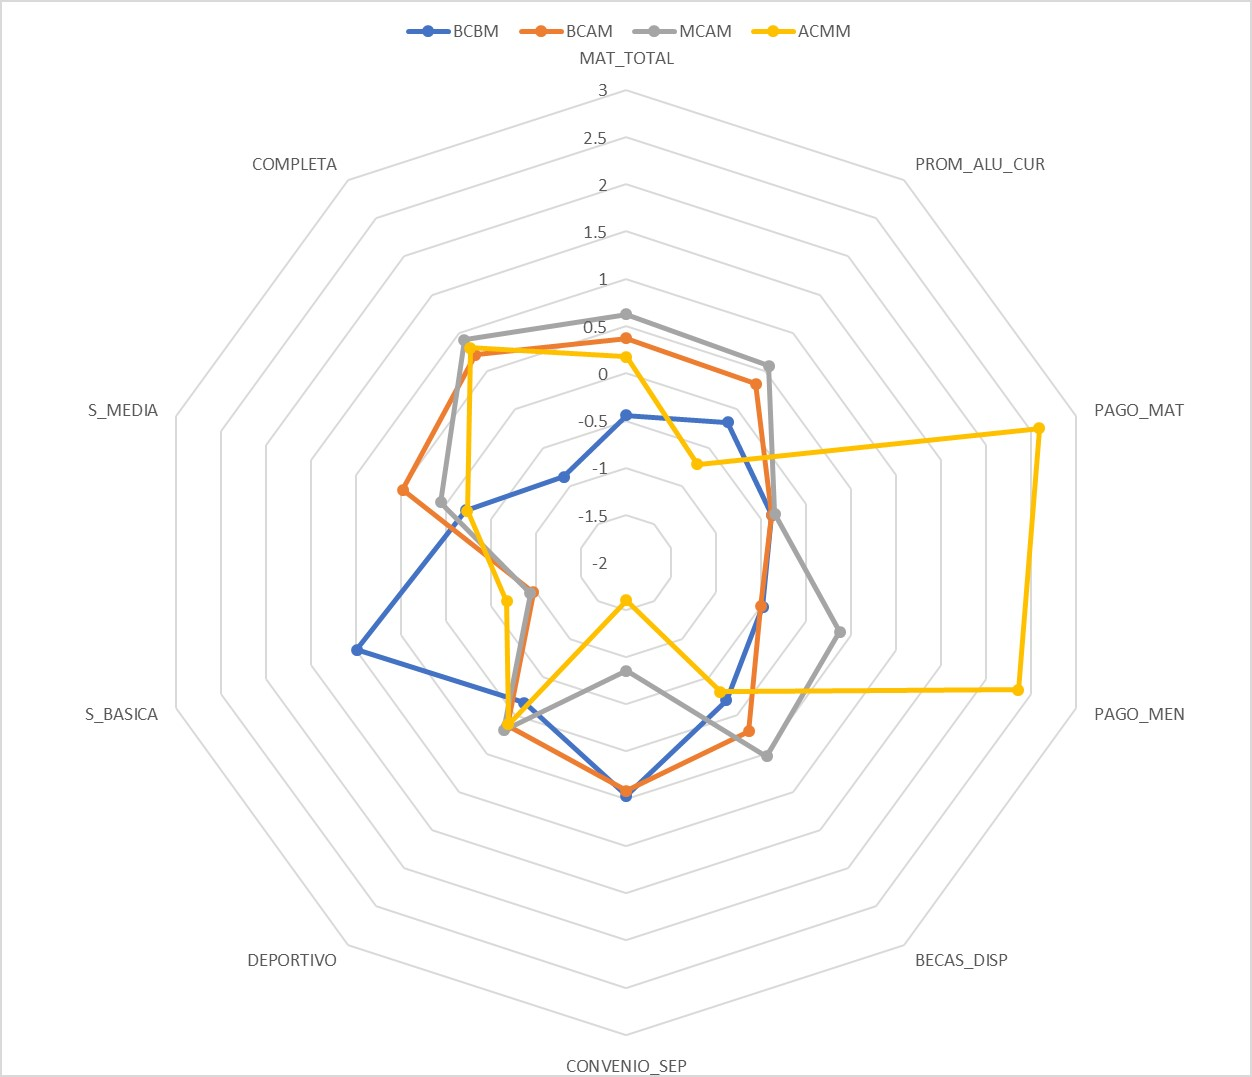
\includegraphics[width=0.66\textwidth]{images/radar_chart_establecimientos_sin.jpg}
    \caption{Promedios de atributos normalizados para establecimientos de la Región Metropolitana.}
    \label{fig:radar_estab}
\end{figure}

\begin{figure}[hc]
    \centering
    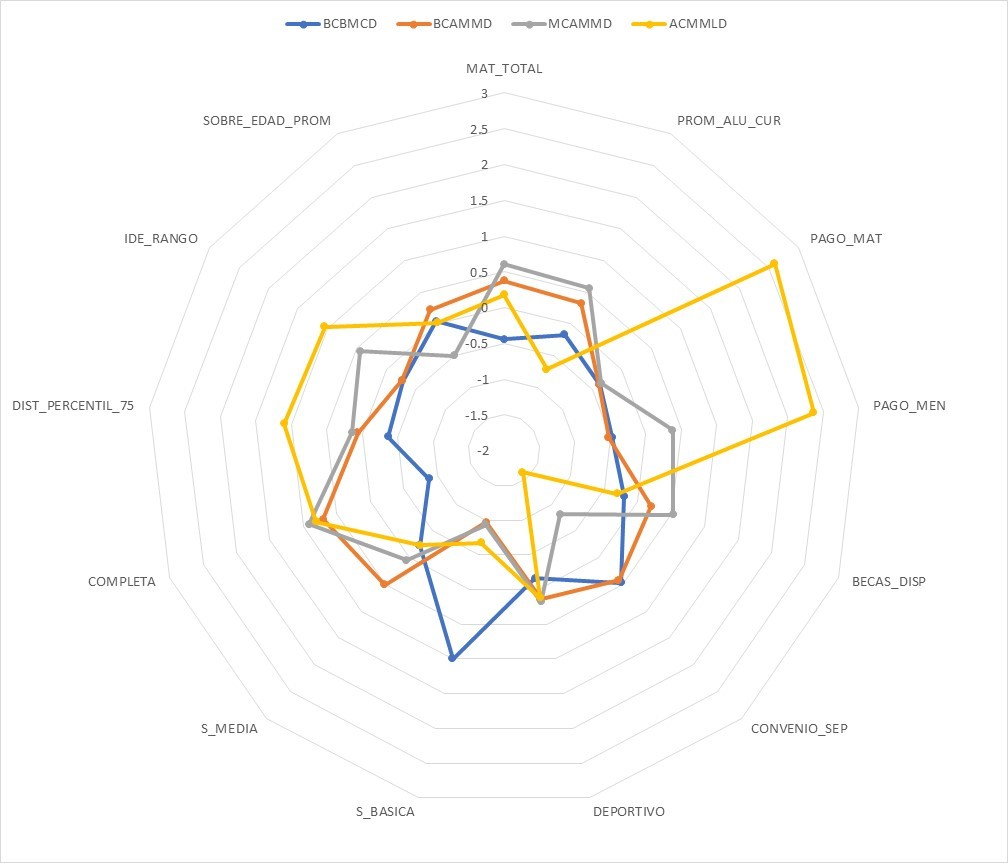
\includegraphics[width=0.66\textwidth]{images/radar_chart_establecimientos_con.jpg}
    \caption{Promedios de atributos normalizados de establecimientos con atributos relacionales (tabla \ref{tab:atributos_relacion_establecimientos}) de la Región Metropolitana.}
    \label{fig:radar_estab_rel}
\end{figure}

Los primeros dos clústers son colegios gratuitos o baratos con un IDE bajo que se diferencian entre ellos principalmente por el nivel de educación que imparten, en el primero predominan los de enseñanza básica y en el segundo establecimientos que imparten educación media o completa. El tercer y cuarto clúster se diferencia de los otros dos por tener un nivel de copago e IDE superiores, donde en el tercero se tienen valores medios y en el cuarto valores elevados. Por otro lado, al analizar la distancia que separa a los establecimientos de sus estudiantes, se aprecia notoriamente que el desplazamiento crece al aumentar el nivel del copago. Es decir, las familias que más pagan están dispuestas a desplazarse distancias mayores para llegar al establecimiento en comparación a familias que optan por colegios gratuitos o de bajo costo. Finalmente otro punto interesante de analizar es la sobre edad, que en el caso de los colegios más caros se concentra con un 95\% en un año de sobre edad. En el resto de los clústers el valor fluctúa entre un 75\% y 85\%, y el resto de distribuye de 2 a 4 años de sobre edad.

Para el caso de las matrículas lo primero que se debe analizar es la tabla \ref{tab:cl_mat}, en donde se aprecian los resultados de las 3 ejecuciones con los diferentes atributos, agrupados por su nivel de importancia. Se puede ver que las primeras dos ejecuciones generan clústers de cardinalidad muy similares, diferenciándose claramente con el tercer resultado, el cual presenta clústers de tamaños similares. La diferencia se en que los clústers de la última ejecución poseen atributos que describen de mejor manera los grupos, los cuales se van perdiendo al ir añadiendo atributos adicionales. 

Además de lo ya mencionado, es importante tener en cuenta que agregar más atributos a una base de datos de un total de 1.500.000 registros aproximadamente, provocará que el tiempo requerido para su ejecución aumenta significativamente. Por lo tanto, se analizarán más a fondo los resultados de la tercera ejecución y se utilizará para comparar con los resultados que se obtienen al agregar los atributos de relación.

Lo siguiente a analizar son las diferentes características de los clústers obtenidos para las matrículas y compararlos con los que se obtienen cuando se incluyen los atributos de relación. Para facilitar la comparación entre clústers se generaron las figuras \ref{fig:chart_mat} y \ref{fig:radar_mat_rel}.

En la primera instancia, se aprecian 2 atributos que generan la mayor categorización dentro de los clústers y que permiten etiquetar al grupo. Estos atributos, el género y el ser o no beneficiario SEP, son del tipo binarios y al ser combinados generan los 4 clústers obtenidos. Es decir, al grupo que pertenezca un alumno se basa principalmente en si es hombre o mujer y si tiene o no la subvención escolar preferencial.

Otro aspecto importante que se aprecia en los clústers generados es que en los grupos de mujeres el nivel de sobre edad es menor a su símil masculino. Esto se puede ver con mayor precisión en la tabla \ref{tab:cl_mat_sobre_edad}, en donde los porcentajes de matrículas con sobre edad mayor o igual a un año es mayor en los clústers de hombres. Al analizar los porcentajes por años de sobre edad, estos tienen una distribución similar, aunque los porcentajes del género femenino tienden a ser mayores para 1 año y menores para 2 o más años.

\begin{figure}[hc]
    \centering
    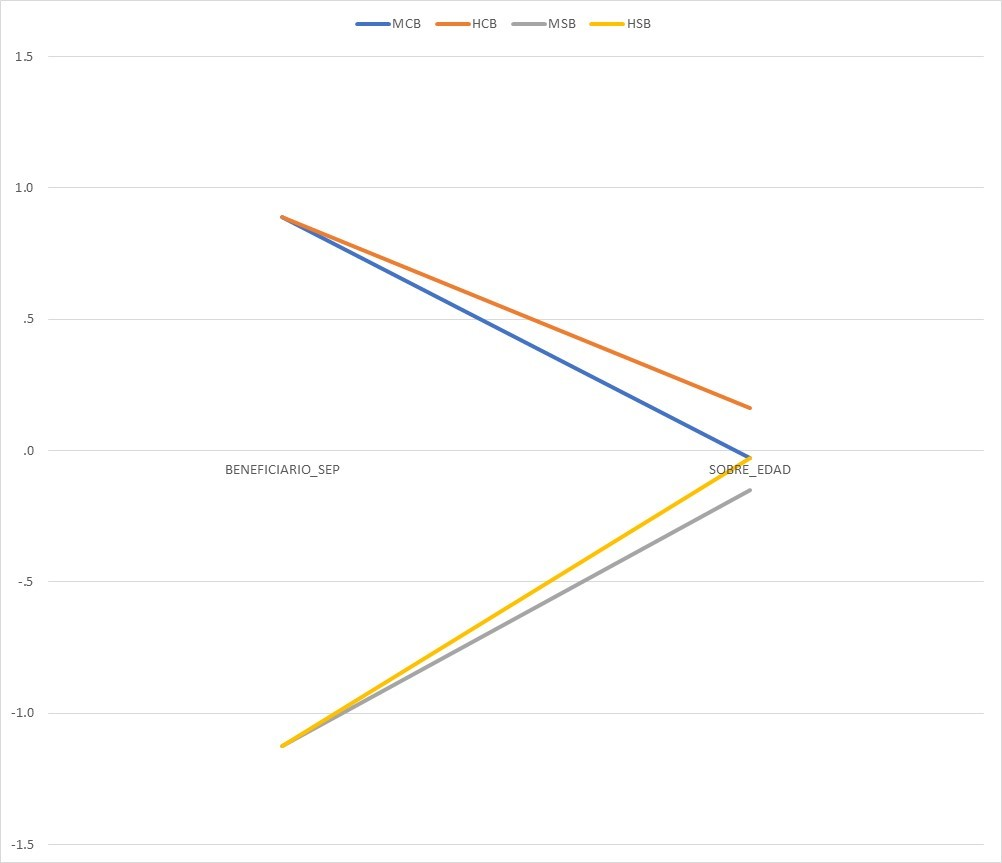
\includegraphics[width=0.66\textwidth]{images/chart_matriculas_sin.jpg}
    \caption{Promedio de atributos normalizados de matrículas de la Región Metropolitana.}
    \label{fig:chart_mat}
\end{figure}

\begin{figure}[H]
    \centering
    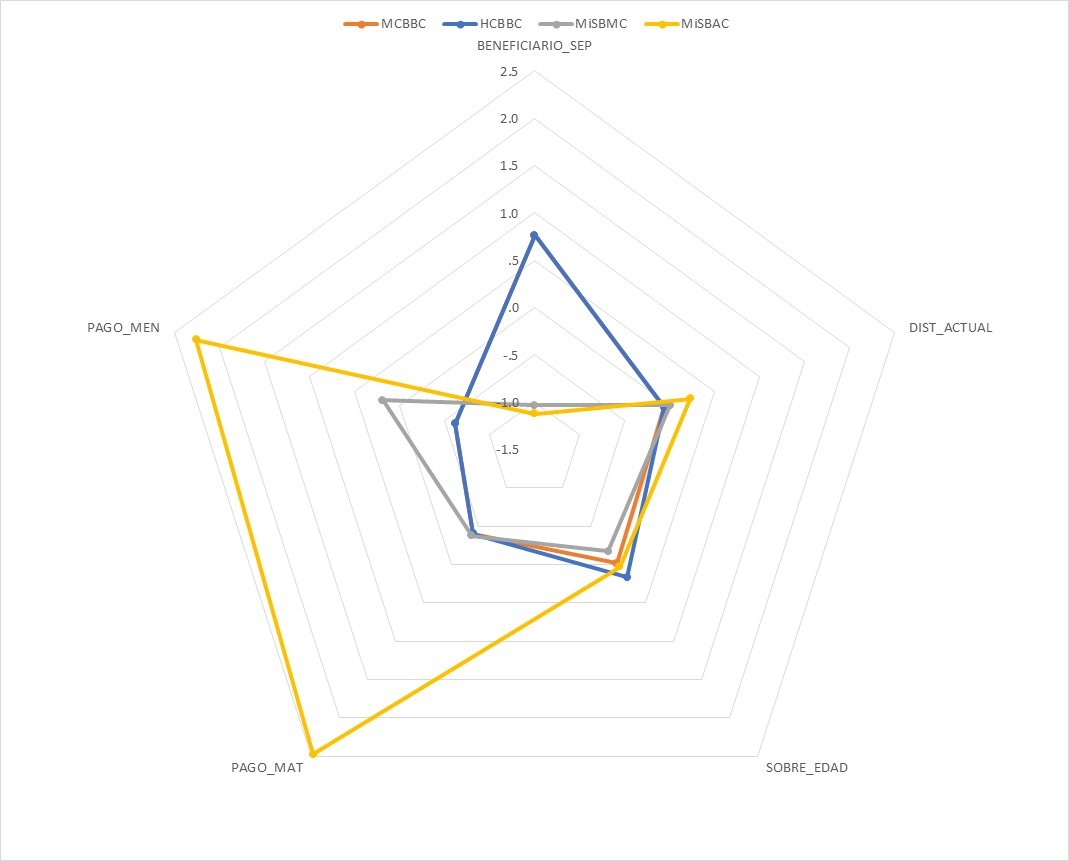
\includegraphics[width=0.66\textwidth]{images/radar_chart_matriculas_con.jpg}
    \caption{Promedio de atributos normalizados de matrículas con atributos relacionales (tabla \ref{tab:atributos_relacion_matriculas}) de la Región Metropolitana.}
    \label{fig:radar_mat_rel}
\end{figure}

Al momento de incluir los atributos de relación (nivel de copago y distancia al establecimiento), los atributos más relevantes siguen siendo el género y el ser o no beneficiario del SEP, sumándose a estos el nivel de copago. A pesar de esto se debe destacar que la importancia del género no es la misma que en la situación anterior, debido a que en este caso 2 de los 4 clústers no son excluyentes en este atributo, grupos en los que cobra mas importancia el nivel de copago.

Los primeros dos grupos presentan características similares a los de la primera prueba, incorporando como atributo principal el nivel de copago, que para ambos es gratuito. Además para estos grupos se mantiene constante el hecho de que las mujeres presentan un nivel de sobre edad menor al de los varones. Como se mencionó anteriormente, el tercer y cuarto clúster son no excluyentes por género, por lo cual en estos dos pasa a ser más importante el copago. En el tercer clúster el nivel de copago es un costo bajo o medio y en el cuarto es mucho más alto. 

En estos clústers la distancia no es un factor tan determinante para clasificar un alumno en uno u otro grupo, debido a que tienen valores muy similares, los cuales tienen una máxima diferencia de 1 kilómetro.

Es difícil realizar una comparación entre los resultados obtenidos sin incluir los atributos de relación establecimiento-matrícula y los que se obtienen al incluirlos, pero se puede apreciar que en ambos casos el algoritmo clasificó todas las matrículas en 4 clústers. También se puede señalar que el género es importante en este estudio, independiente de que en uno de los resultados tenga menor importancia.


\subsection{Análisis geográfico}

Una vez realizado el análisis cualitativo de los clústers, y con los datos geográficos disponibles, se analiza la distribución geográfica y socioeconómica en el área metropolitana de los clústers de establecimientos, de matrículas y de las matrículas en los clústers de establecimientos.

En la figura \ref{f:mapas_estab_con_gse} se muestra la distribución de los establecimientos de cada clústers en la Región Metropolitana, incluyendo los grupos socioeconómicos. En el mapa de la figura \ref{f:mapa_estab_con_0} se aprecia que los establecimientos del clúster BCBMPD se encuentran distribuidos de manera uniforme sobre gran parte del área metropolitana, exceptuando la zona oriente. Estos se concentran principalmente en las zonas de color naranjo, las cuales corresponden a los GSE de los deciles 3 al 7. Los establecimientos del clúster BCAMMD (figura \ref{f:mapa_estab_con_1}) se distribuyen de la misma forma descrita anteriormente, con la diferencia de que su cardinalidad es menor, por lo cual los colegios se encuentran a una mayor distancia entre ellos.

\begin{figure}[H]
 \centering
  \subfloat[Establecimientos clúster BCBMPD.]{
   \label{f:mapa_estab_con_0}
    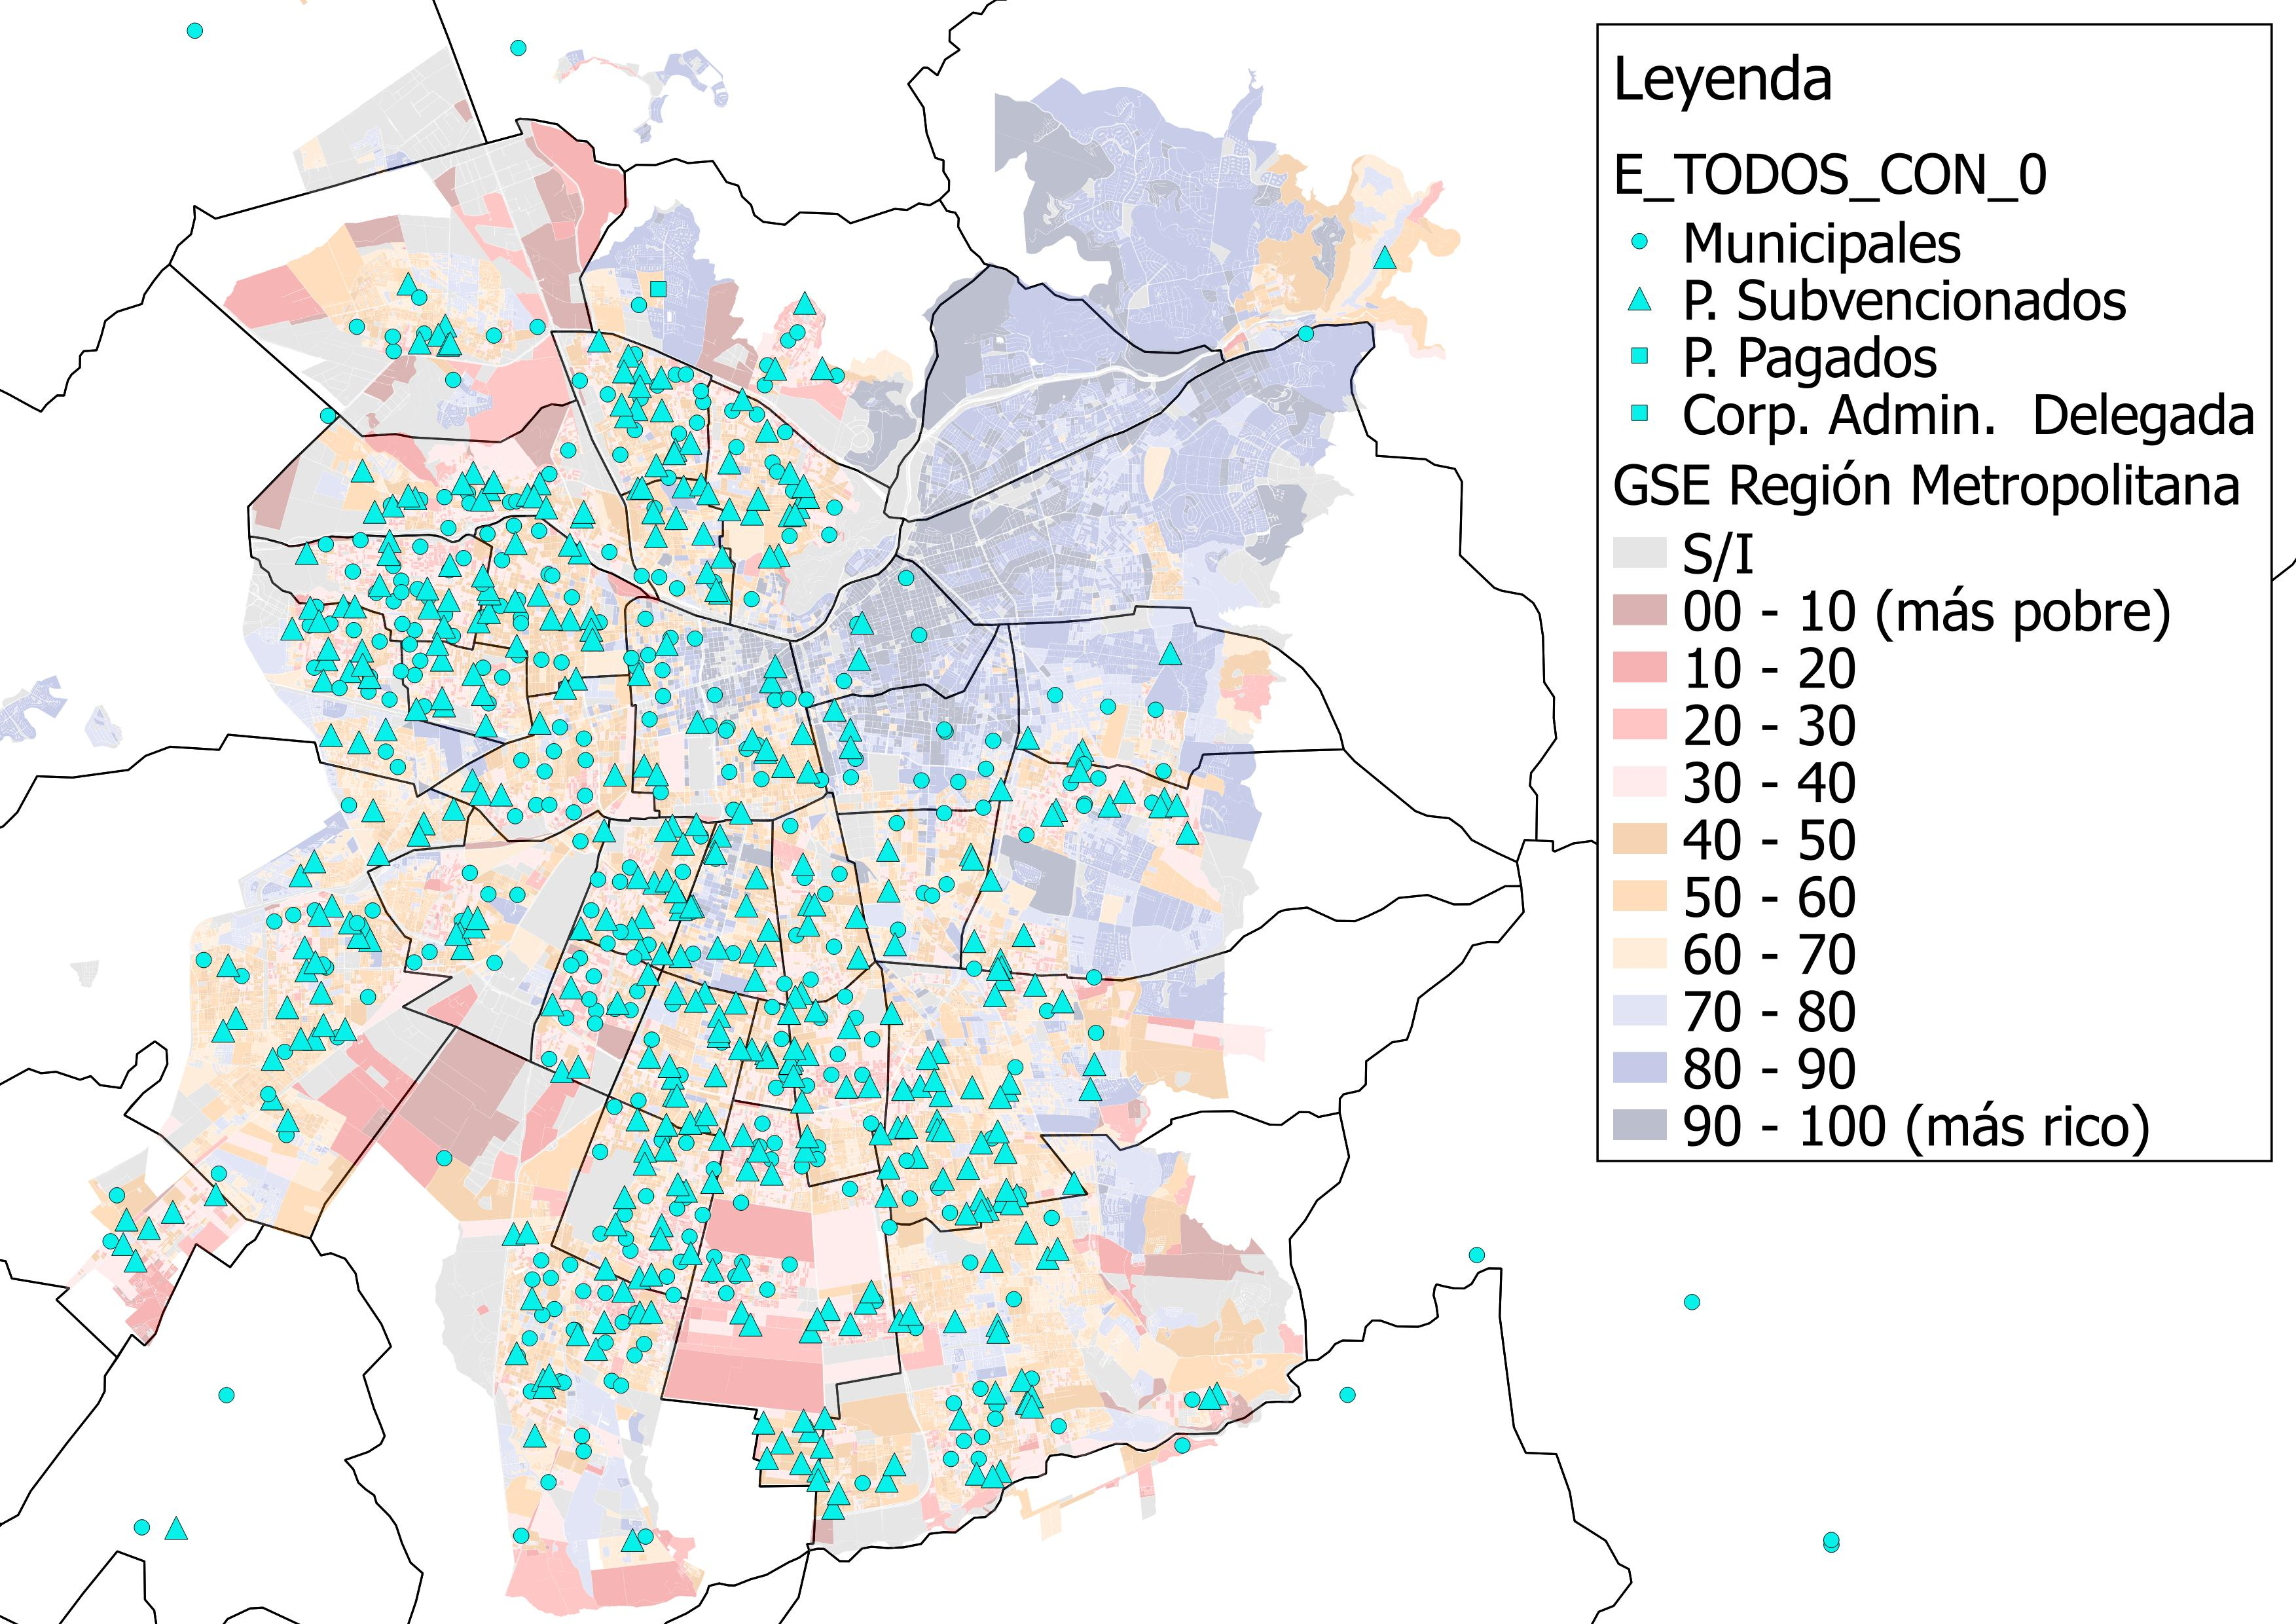
\includegraphics[width=7.5cm]{images/establecimientos/E_TODOS_CON_0.jpg}}
  \subfloat[Establecimientos clúster BCAMMD.]{
   \label{f:mapa_estab_con_1}
    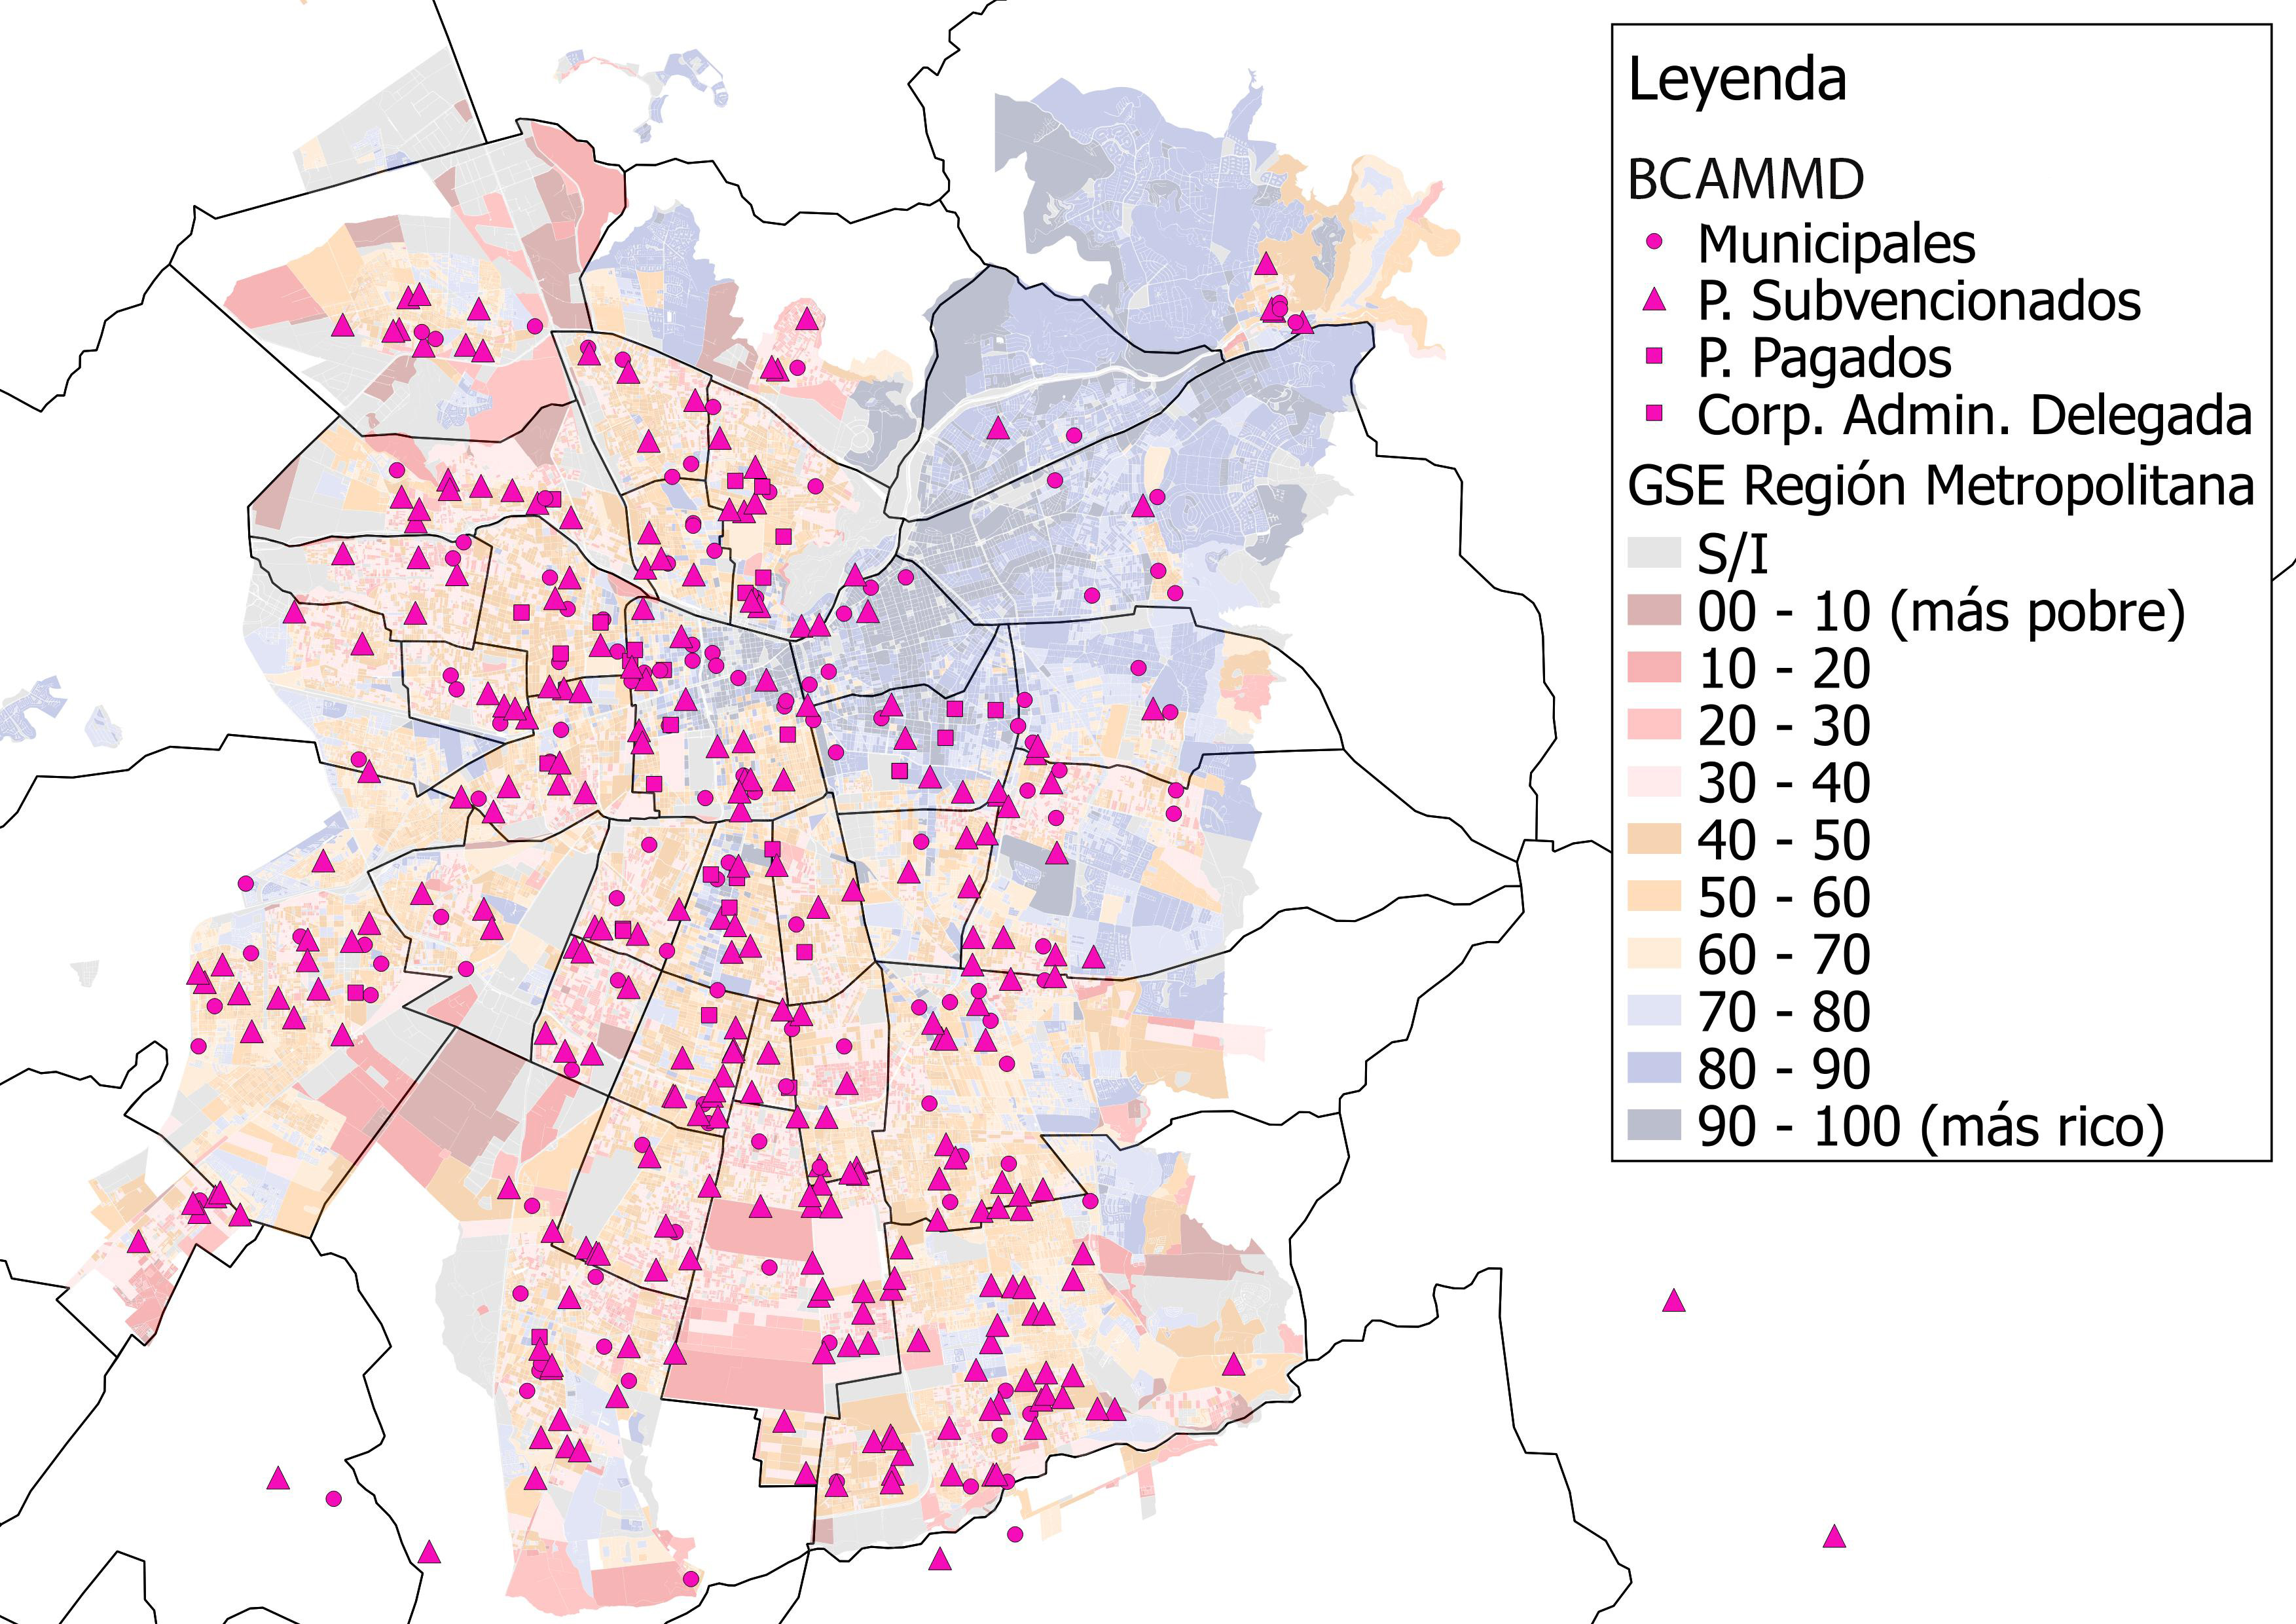
\includegraphics[width=7.5cm]{images/establecimientos/E_TODOS_CON_1.jpg}}\hspace{1mm}
  \subfloat[Establecimientos clúster MCAMMD.]{
   \label{f:mapa_estab_con_2}
    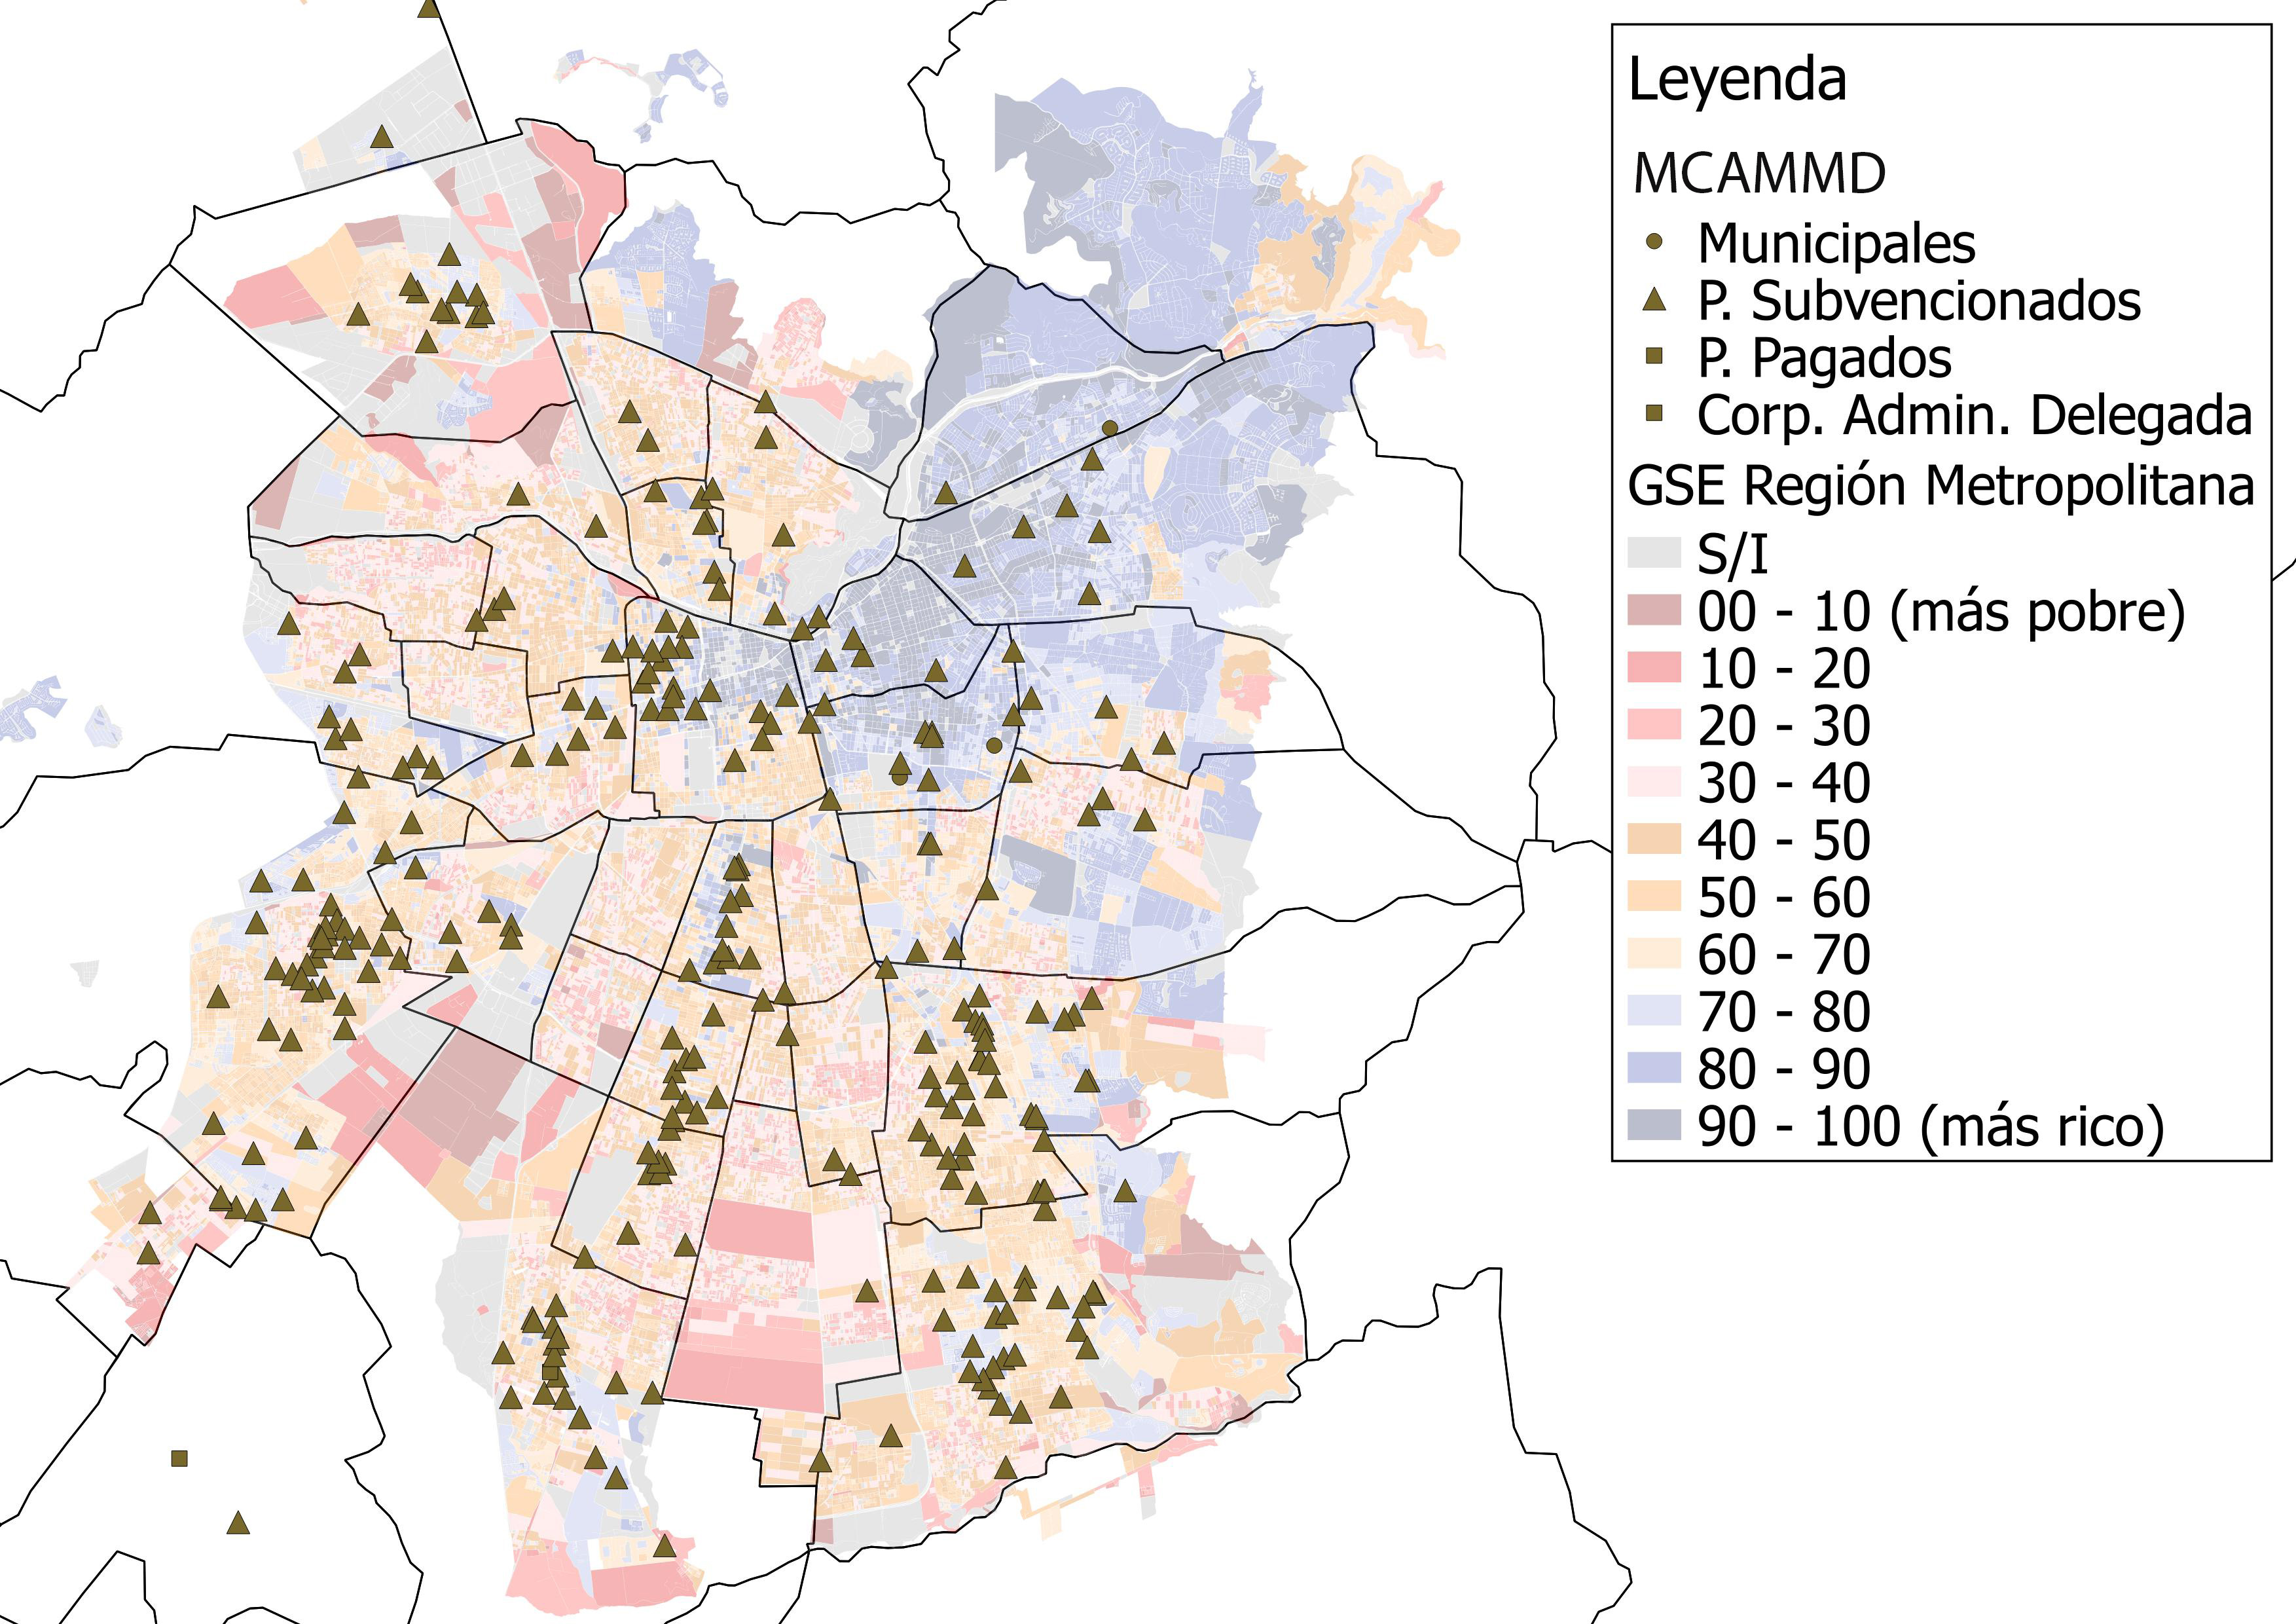
\includegraphics[width=7.5cm]{images/establecimientos/E_TODOS_CON_2.jpg}}
  \subfloat[Establecimientos clúster ACMMLD.]{
   \label{f:mapa_estab_con_3}
    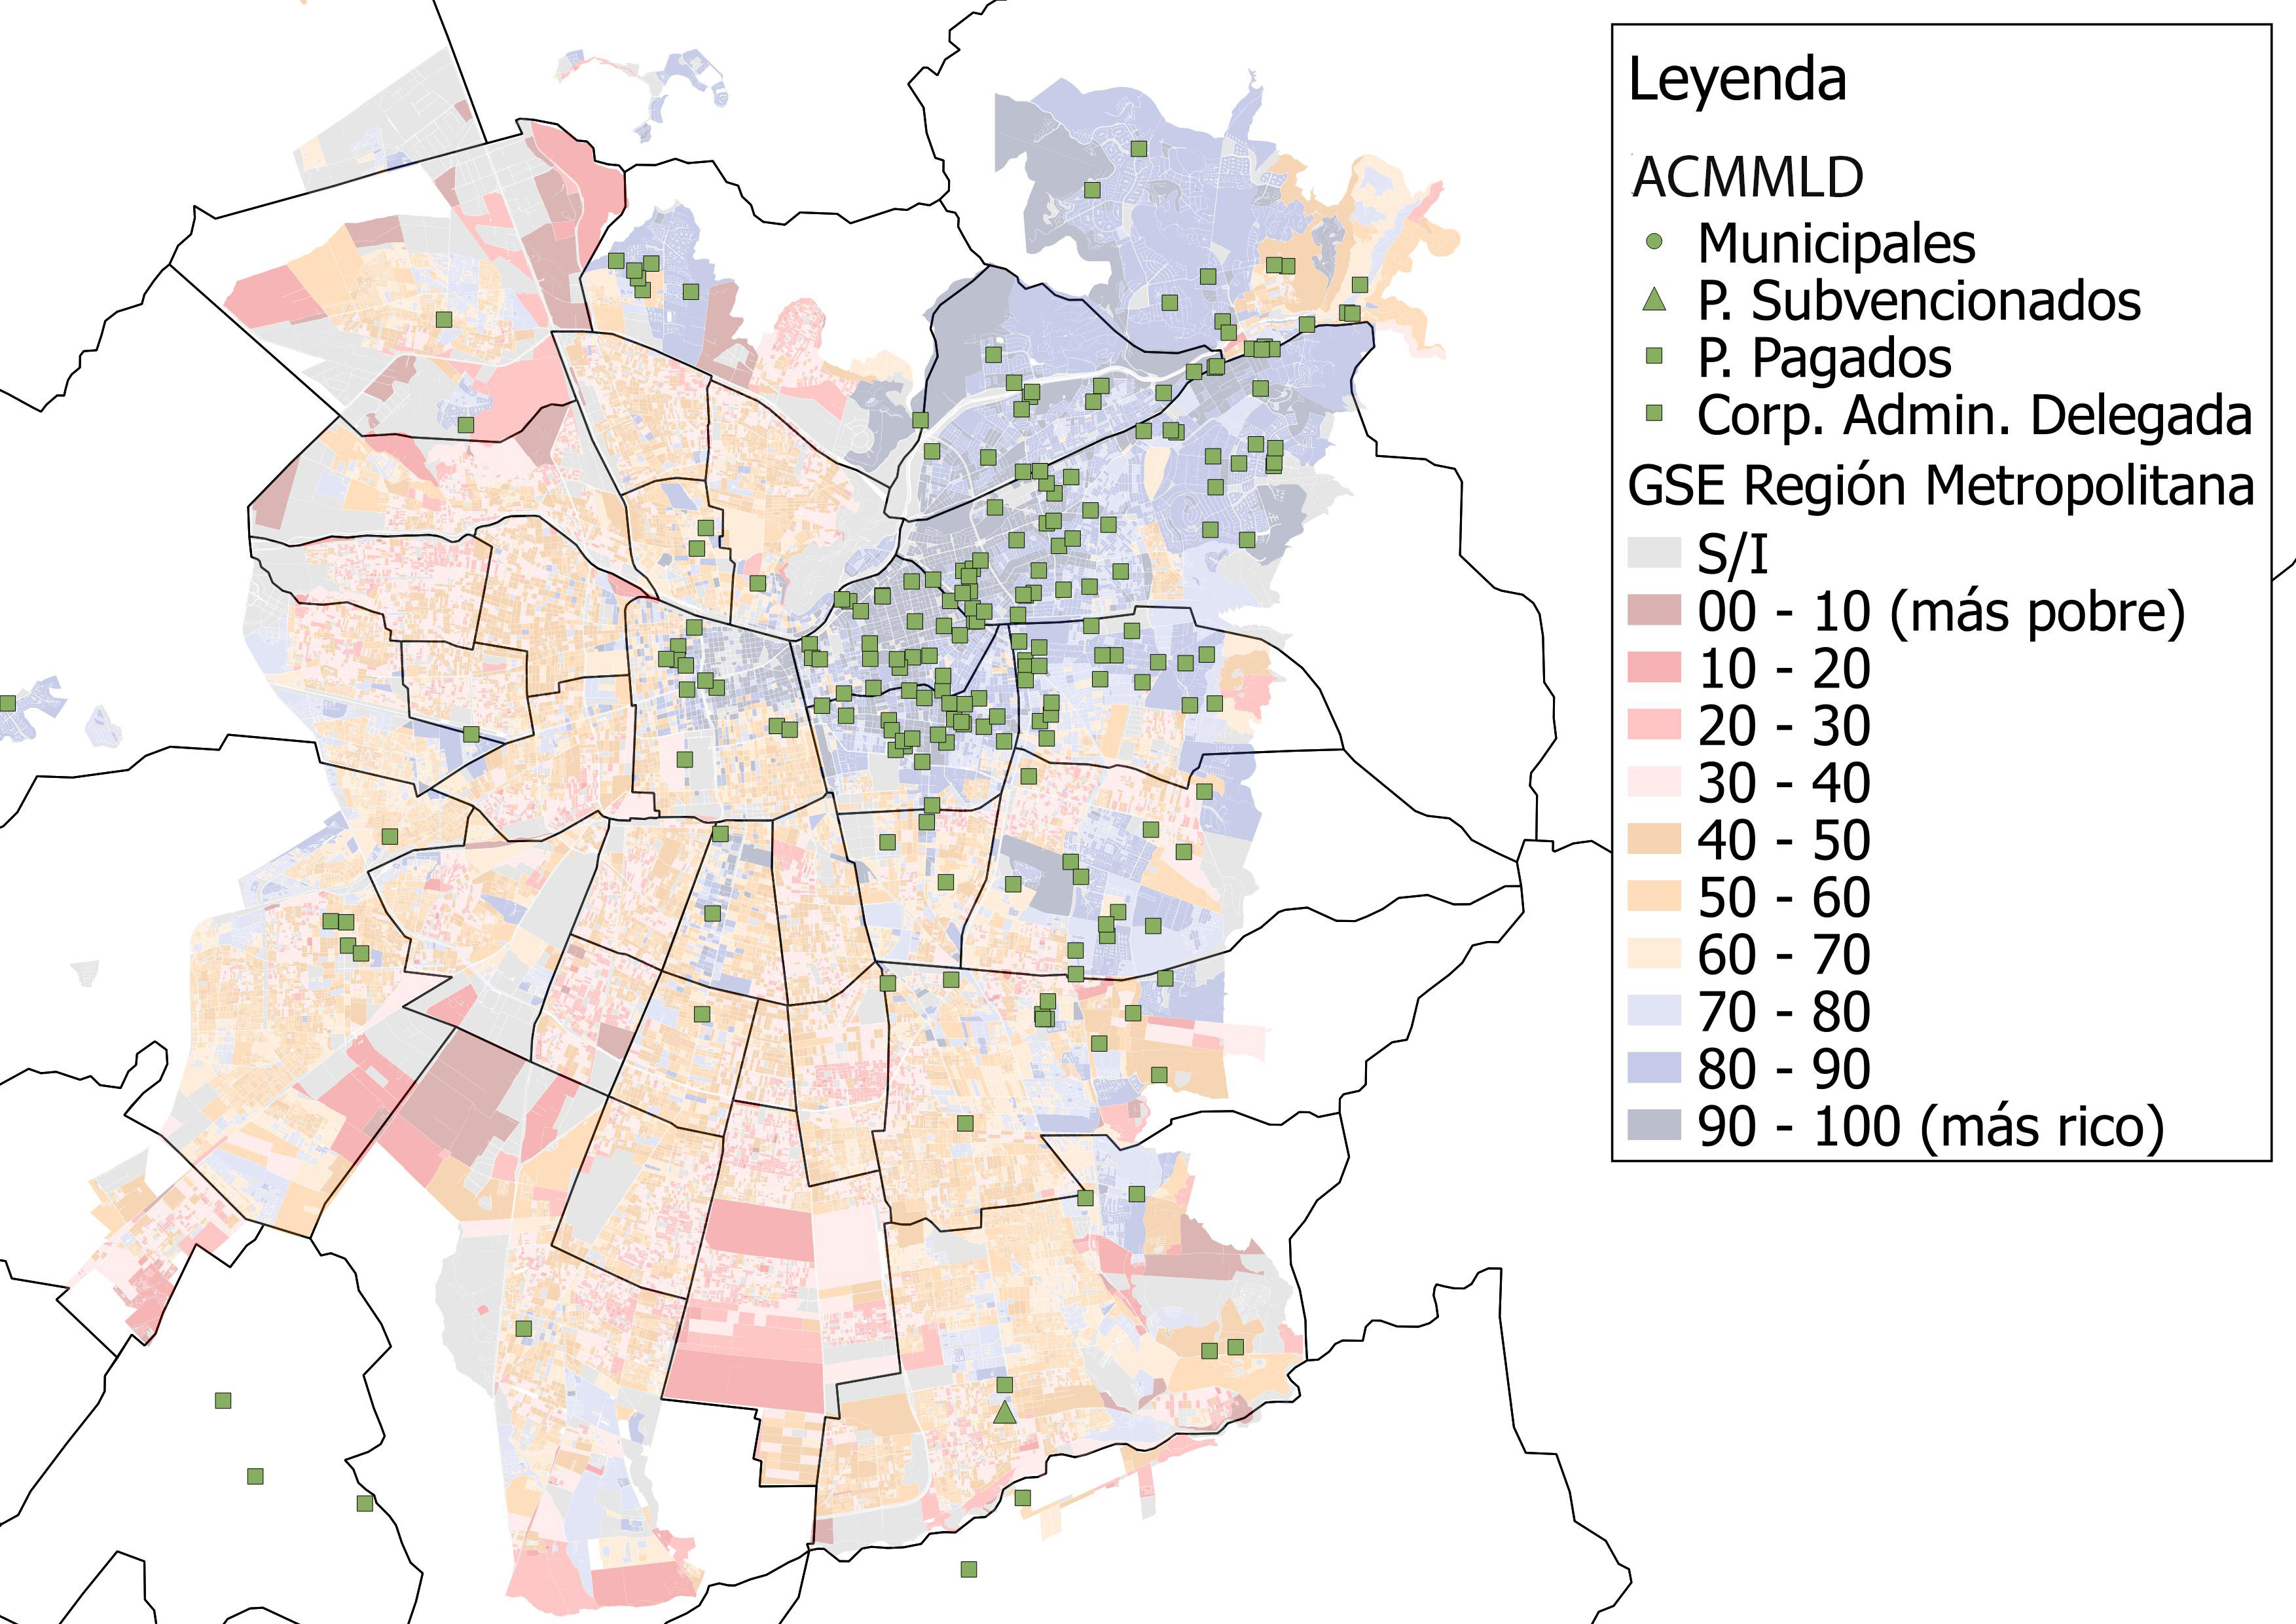
\includegraphics[width=7.5cm]{images/establecimientos/E_TODOS_CON_3.jpg}}
 \caption{Mapas de clústers de establecimientos (con atributos relacionales) sobre mapa GSE de la Región Metropolitana.}
 \label{f:mapas_estab_con_gse}
\end{figure}

\newpage
En la figura \ref{f:mapa_estab_con_2} los colegios del grupo MCAMMD se encuentran ubicados en las zonas anaranjadas, pertenecientes a los deciles 4 al 7. Pero a diferencia de los anteriores, estos se encuentran distribuidos en grupos y no se extienden de manera uniforma por la capital. Por último, el clúster ACMMLD (figura \ref{f:mapa_estab_con_3}) se ubica en la zona oriente de la Región Metropolitana, en donde se encuentran los GSE de mayor ingreso per cápita (deciles del 8 al 10). Esto concuerda con que los establecimientos de este clúster son los que tienen las matrículas y mensualidades más elevadas de la capital.

De manera general se puede apreciar que los establecimientos se encuentran principalmente en el área metropolitana de la capital (zonas coloreadas según su GSE). Además, estos se ubican principalmente en las zonas de colores naranjos y azules, correspondientes a los deciles 3 al 10, dejando a los sectores más pobres (deciles 1 y 2) con una presencia casi nula. Esto, de una u otra manera, refleja la importancia que tiene el grupo socioeconómico sobre la ubicación de un establecimiento y los niveles de costo que tienen.

En los mapas de la figura \ref{f:mapas_mat_en_estab_con_gse}, y utilizando la geolocalización de las matrículas, se muestra la distribución de los alumnos que asisten a los establecimientos de los diferentes clústers. Es decir, en cada mapa se muestran los alumnos pertenecientes a los colegios que conforman los clústers BCBMPD, BCAMMD, MCAMMD y ACMMLD. En el mapa \ref{f:mapa_mat_en_estab_con_0_gse} los alumnos se distribuyen por casi toda el área metropolitana, exceptuando el sector oriente y concentrándose en sectores de la zona sur y poniente. Los estudiantes del clúster BCAMMD (figura \ref{f:mapa_mat_en_estab_con_1_gse} se encuentran en toda el área metropolitana, con menor proporción y densidad en el sector oriente y presentando una mayor densidad en el sur de la capital.

En \ref{f:mapa_mat_en_estab_con_2_gse} el alumnado se encuentra por toda la capital, concentrándose de manera más densa en la periferia del sector poniente y seguida por dos sectores del sur de la capital. Por último, en el cuarto clúster (figura \ref{f:mapa_mat_en_estab_con_3_gse}) todos sus estudiantes se sitúan en el sector oriente, concentrándose en el sector nororiente.

A partir de los mapas de la figura \ref{f:mapas_mat_en_estab_con_gse} y lo anteriormente descrito, se puede apreciar que en el caso de los primeros tres clústers de establecimientos, sus alumnos predominantemente viven en zonas pertenecientes a los deciles del 4 al 7, a diferencia de lo que ocurre con los del último clúster. Los alumnos de colegios pertenecientes al clúster ACMMLD residen casi en su totalidad en sectores de los deciles 8 al 10, es decir, en los sectores donde viven las familias con mayor ingreso per cápita.

\begin{figure}[H]
 \centering
  \subfloat[Matrículas en colegios de BCBMPD.]{
   \label{f:mapa_mat_en_estab_con_0_gse}
    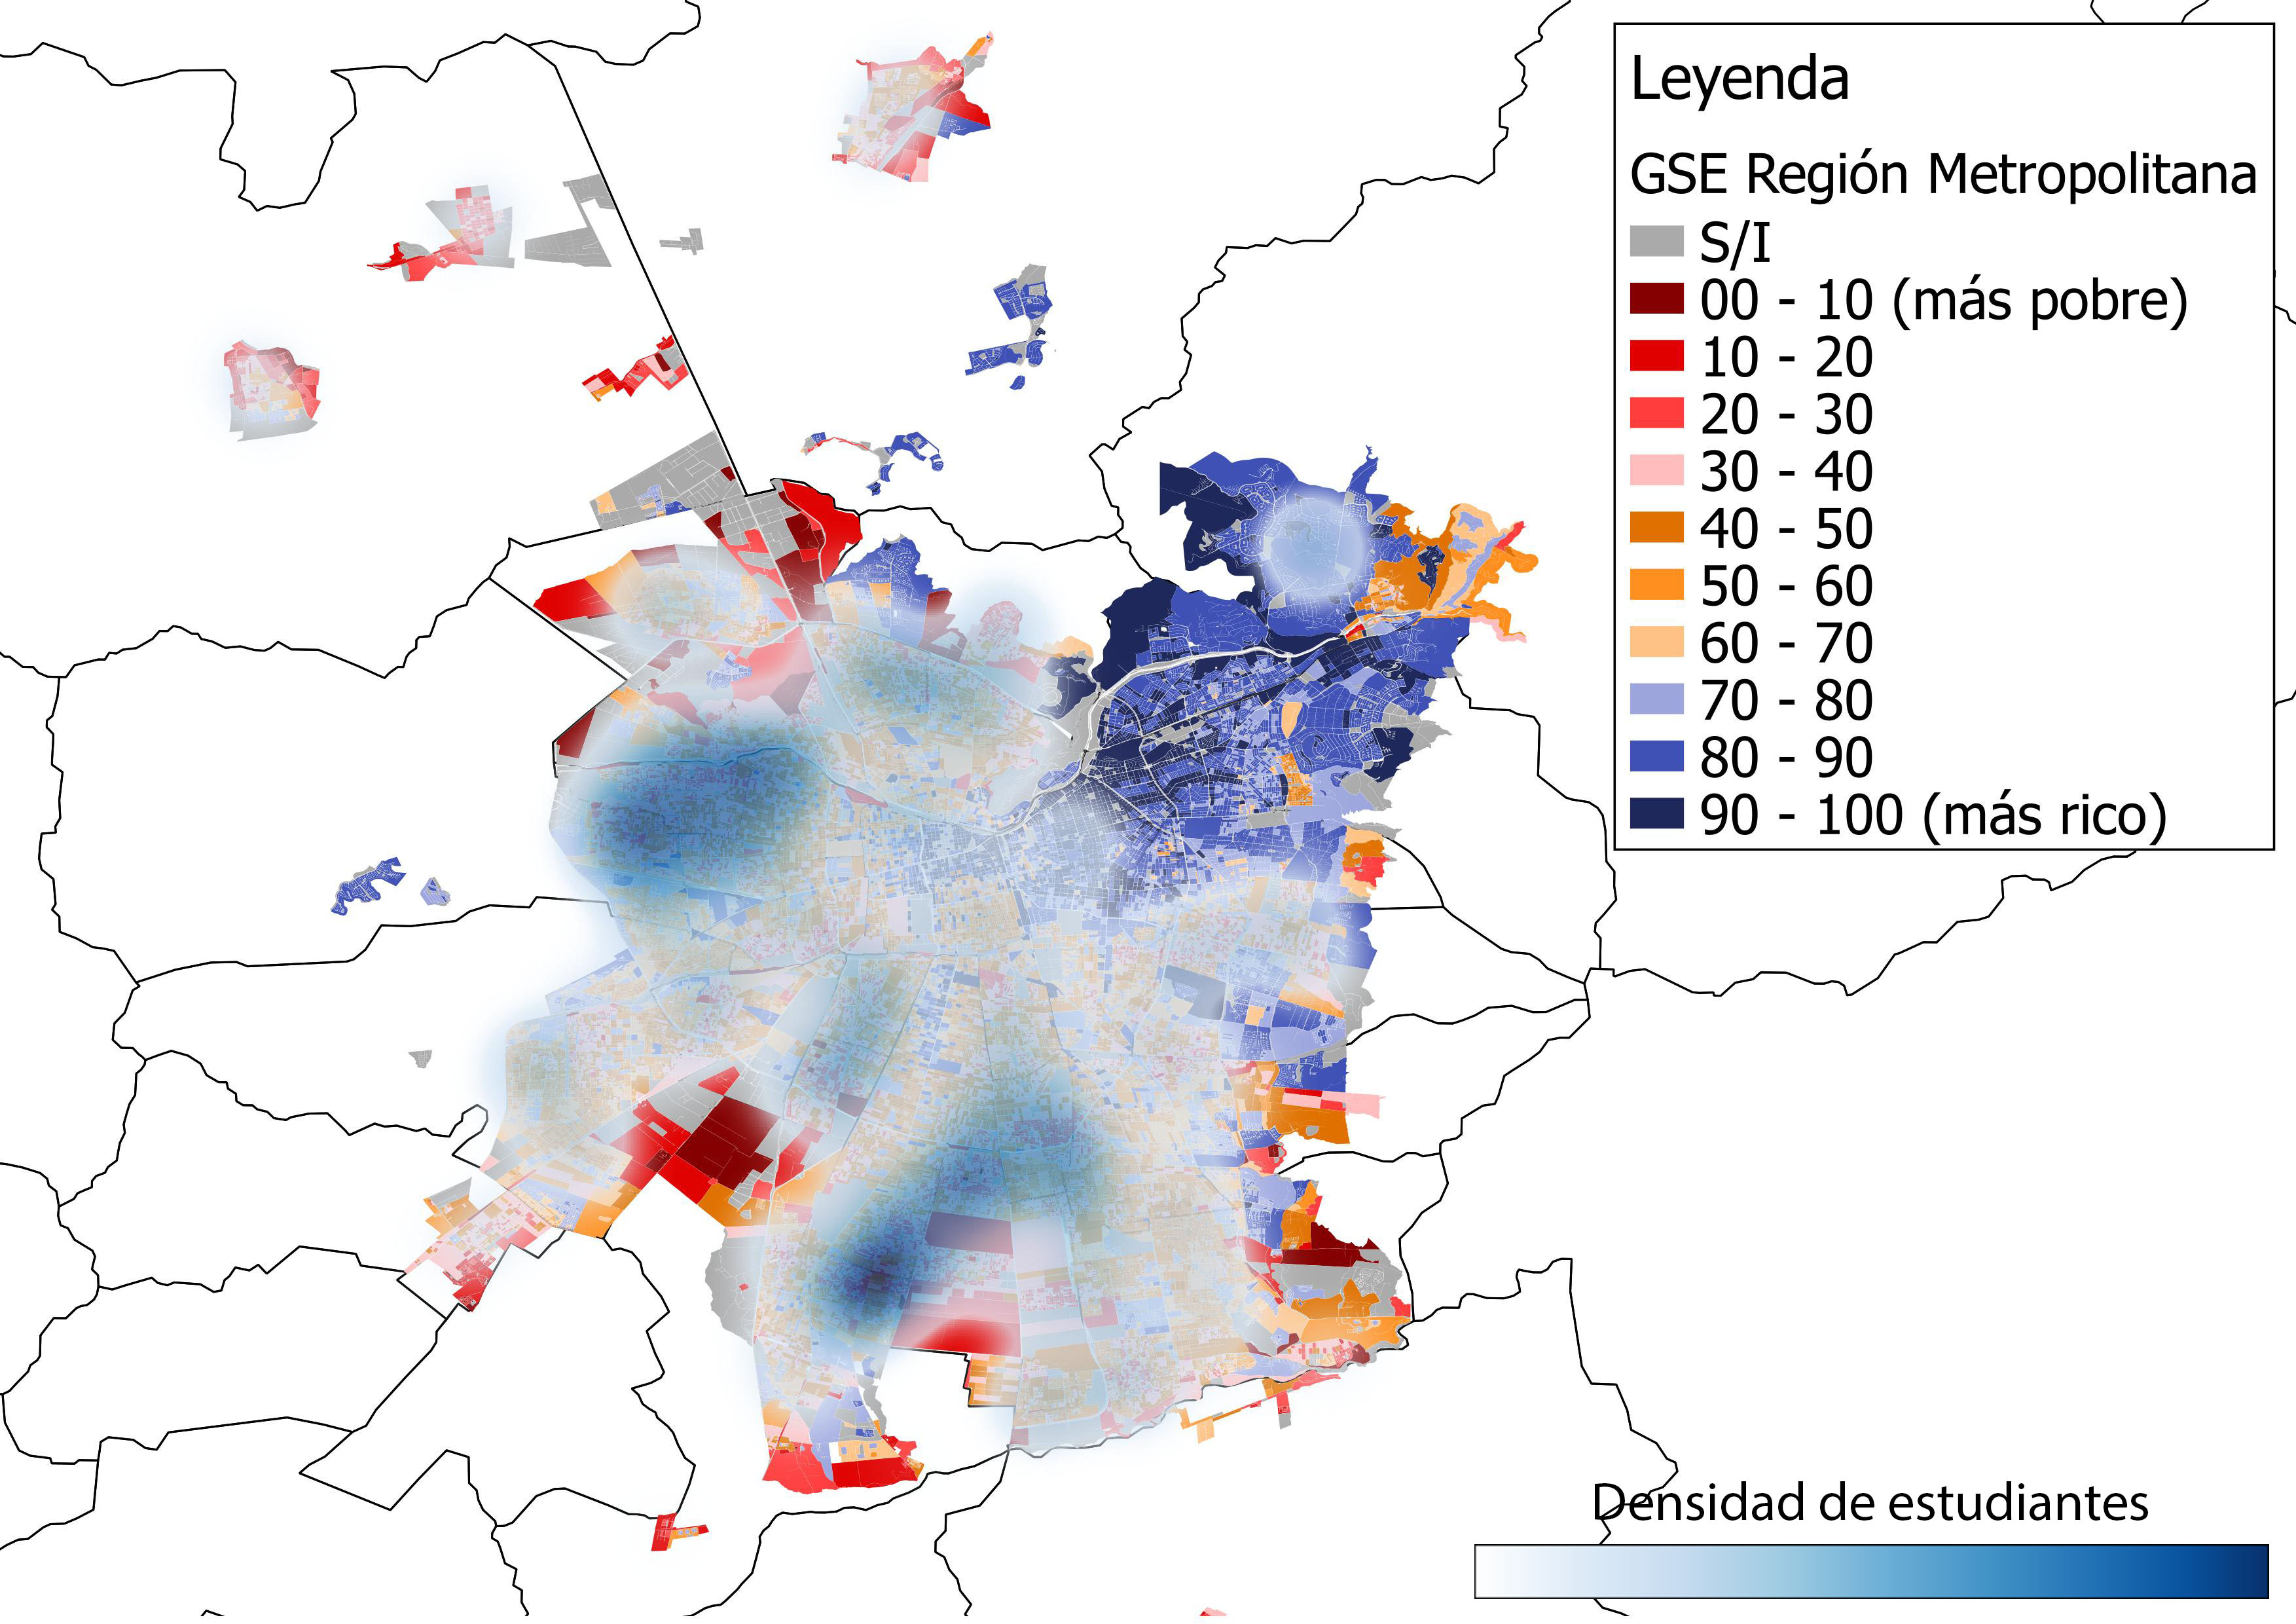
\includegraphics[width=7.5cm]{images/matriculas/E_CON_0_final.jpg}}
  \subfloat[Matrículas en colegios de BCAMMD.]{
   \label{f:mapa_mat_en_estab_con_1_gse}
    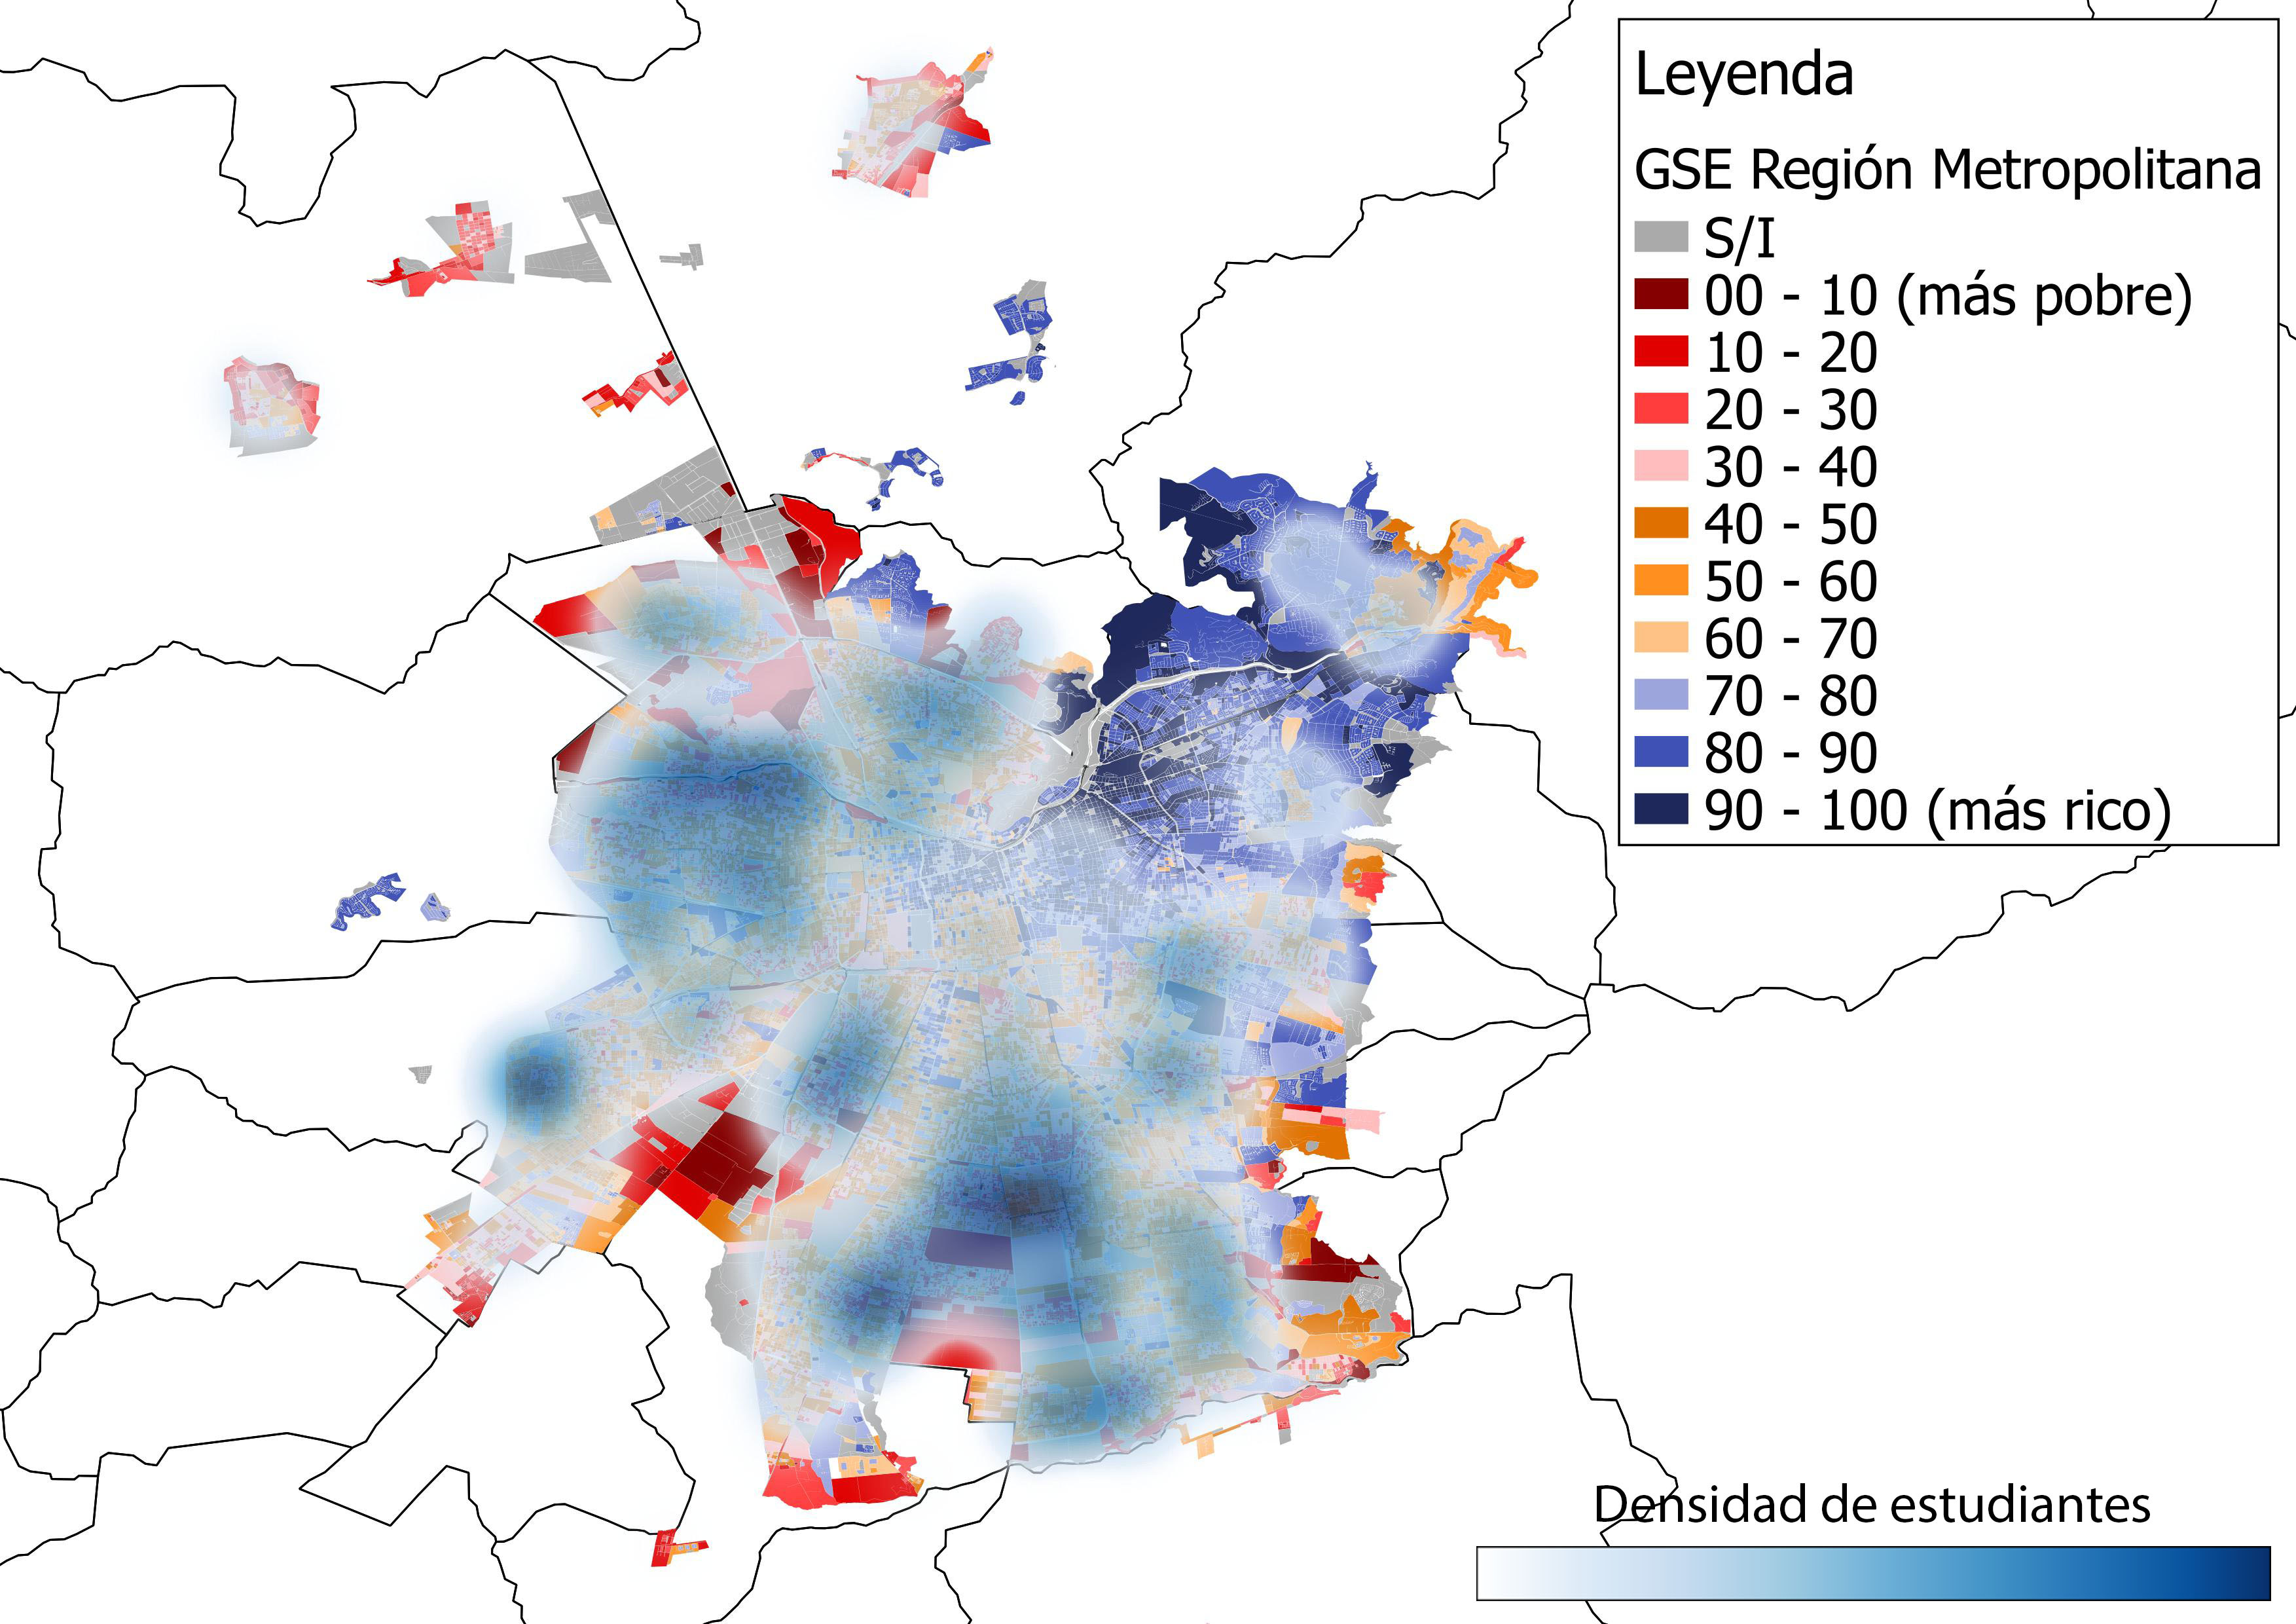
\includegraphics[width=7.5cm]{images/matriculas/E_CON_1_final.jpg}}\hspace{1mm}
  \subfloat[Matrículas en colegios de MCAMMD.]{
   \label{f:mapa_mat_en_estab_con_2_gse}
    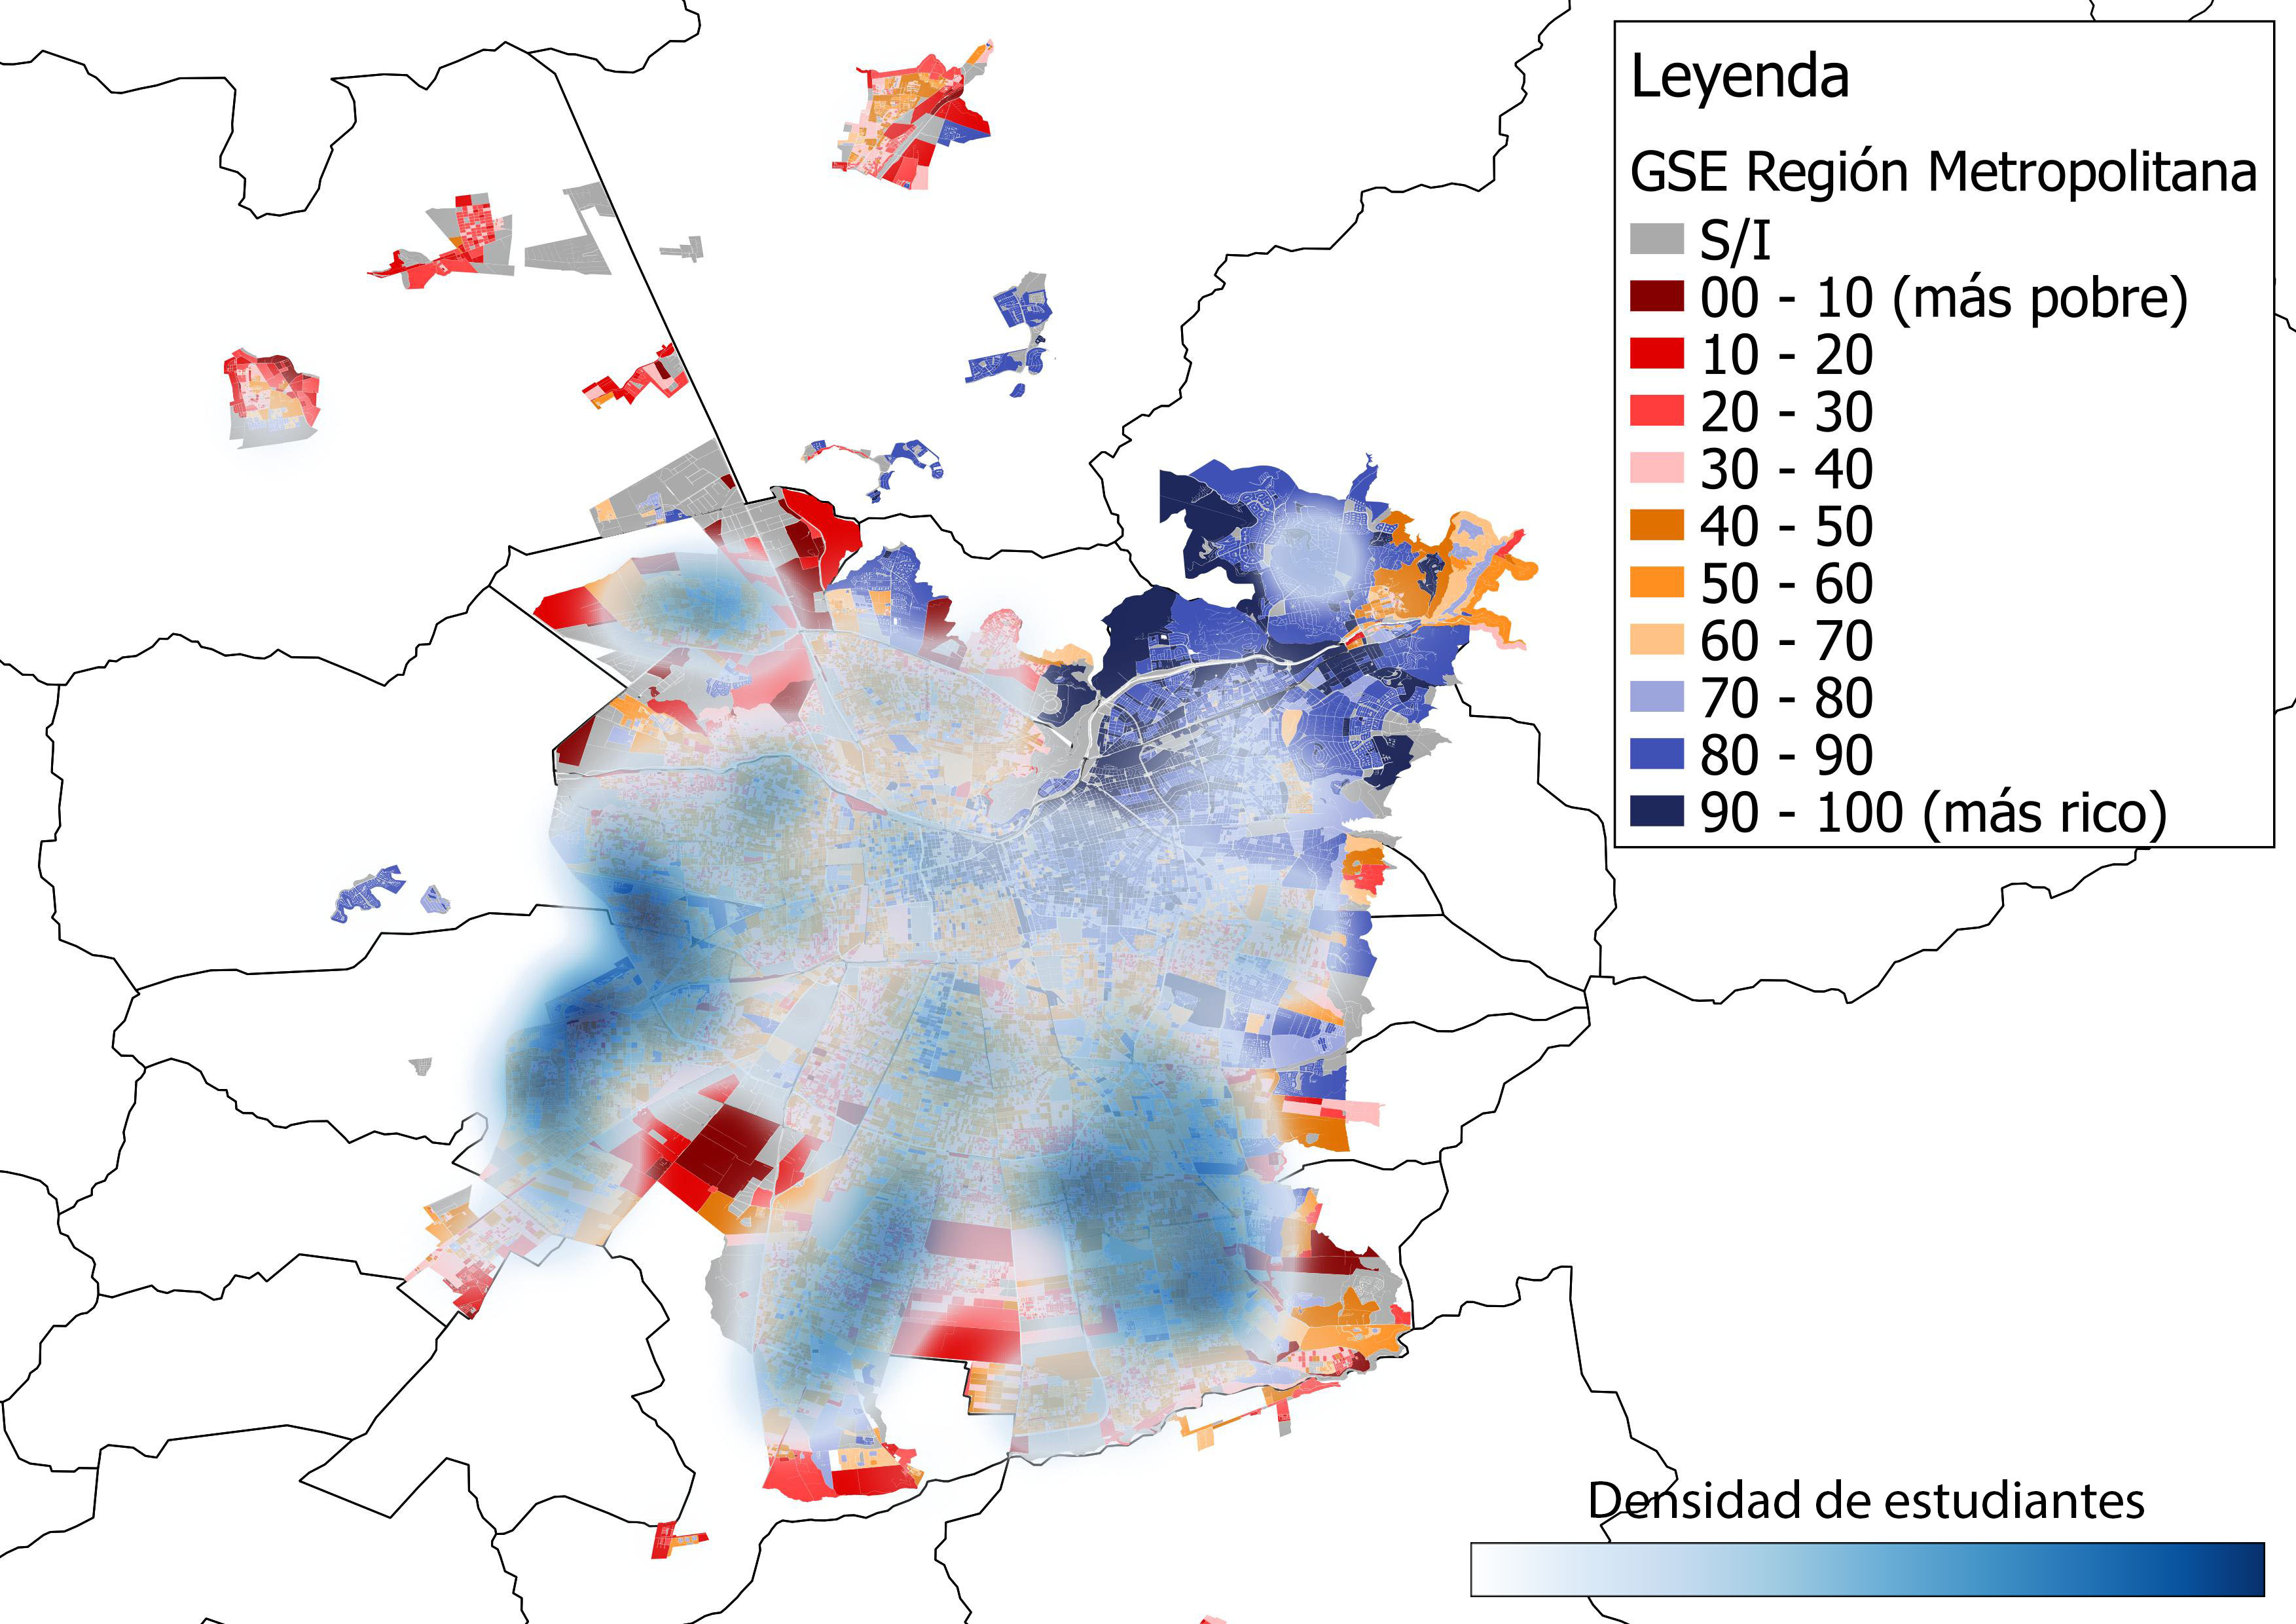
\includegraphics[width=7.5cm]{images/matriculas/E_CON_2_final.jpg}}
  \subfloat[Matrículas en colegios de ACMMLD.]{
   \label{f:mapa_mat_en_estab_con_3_gse}
    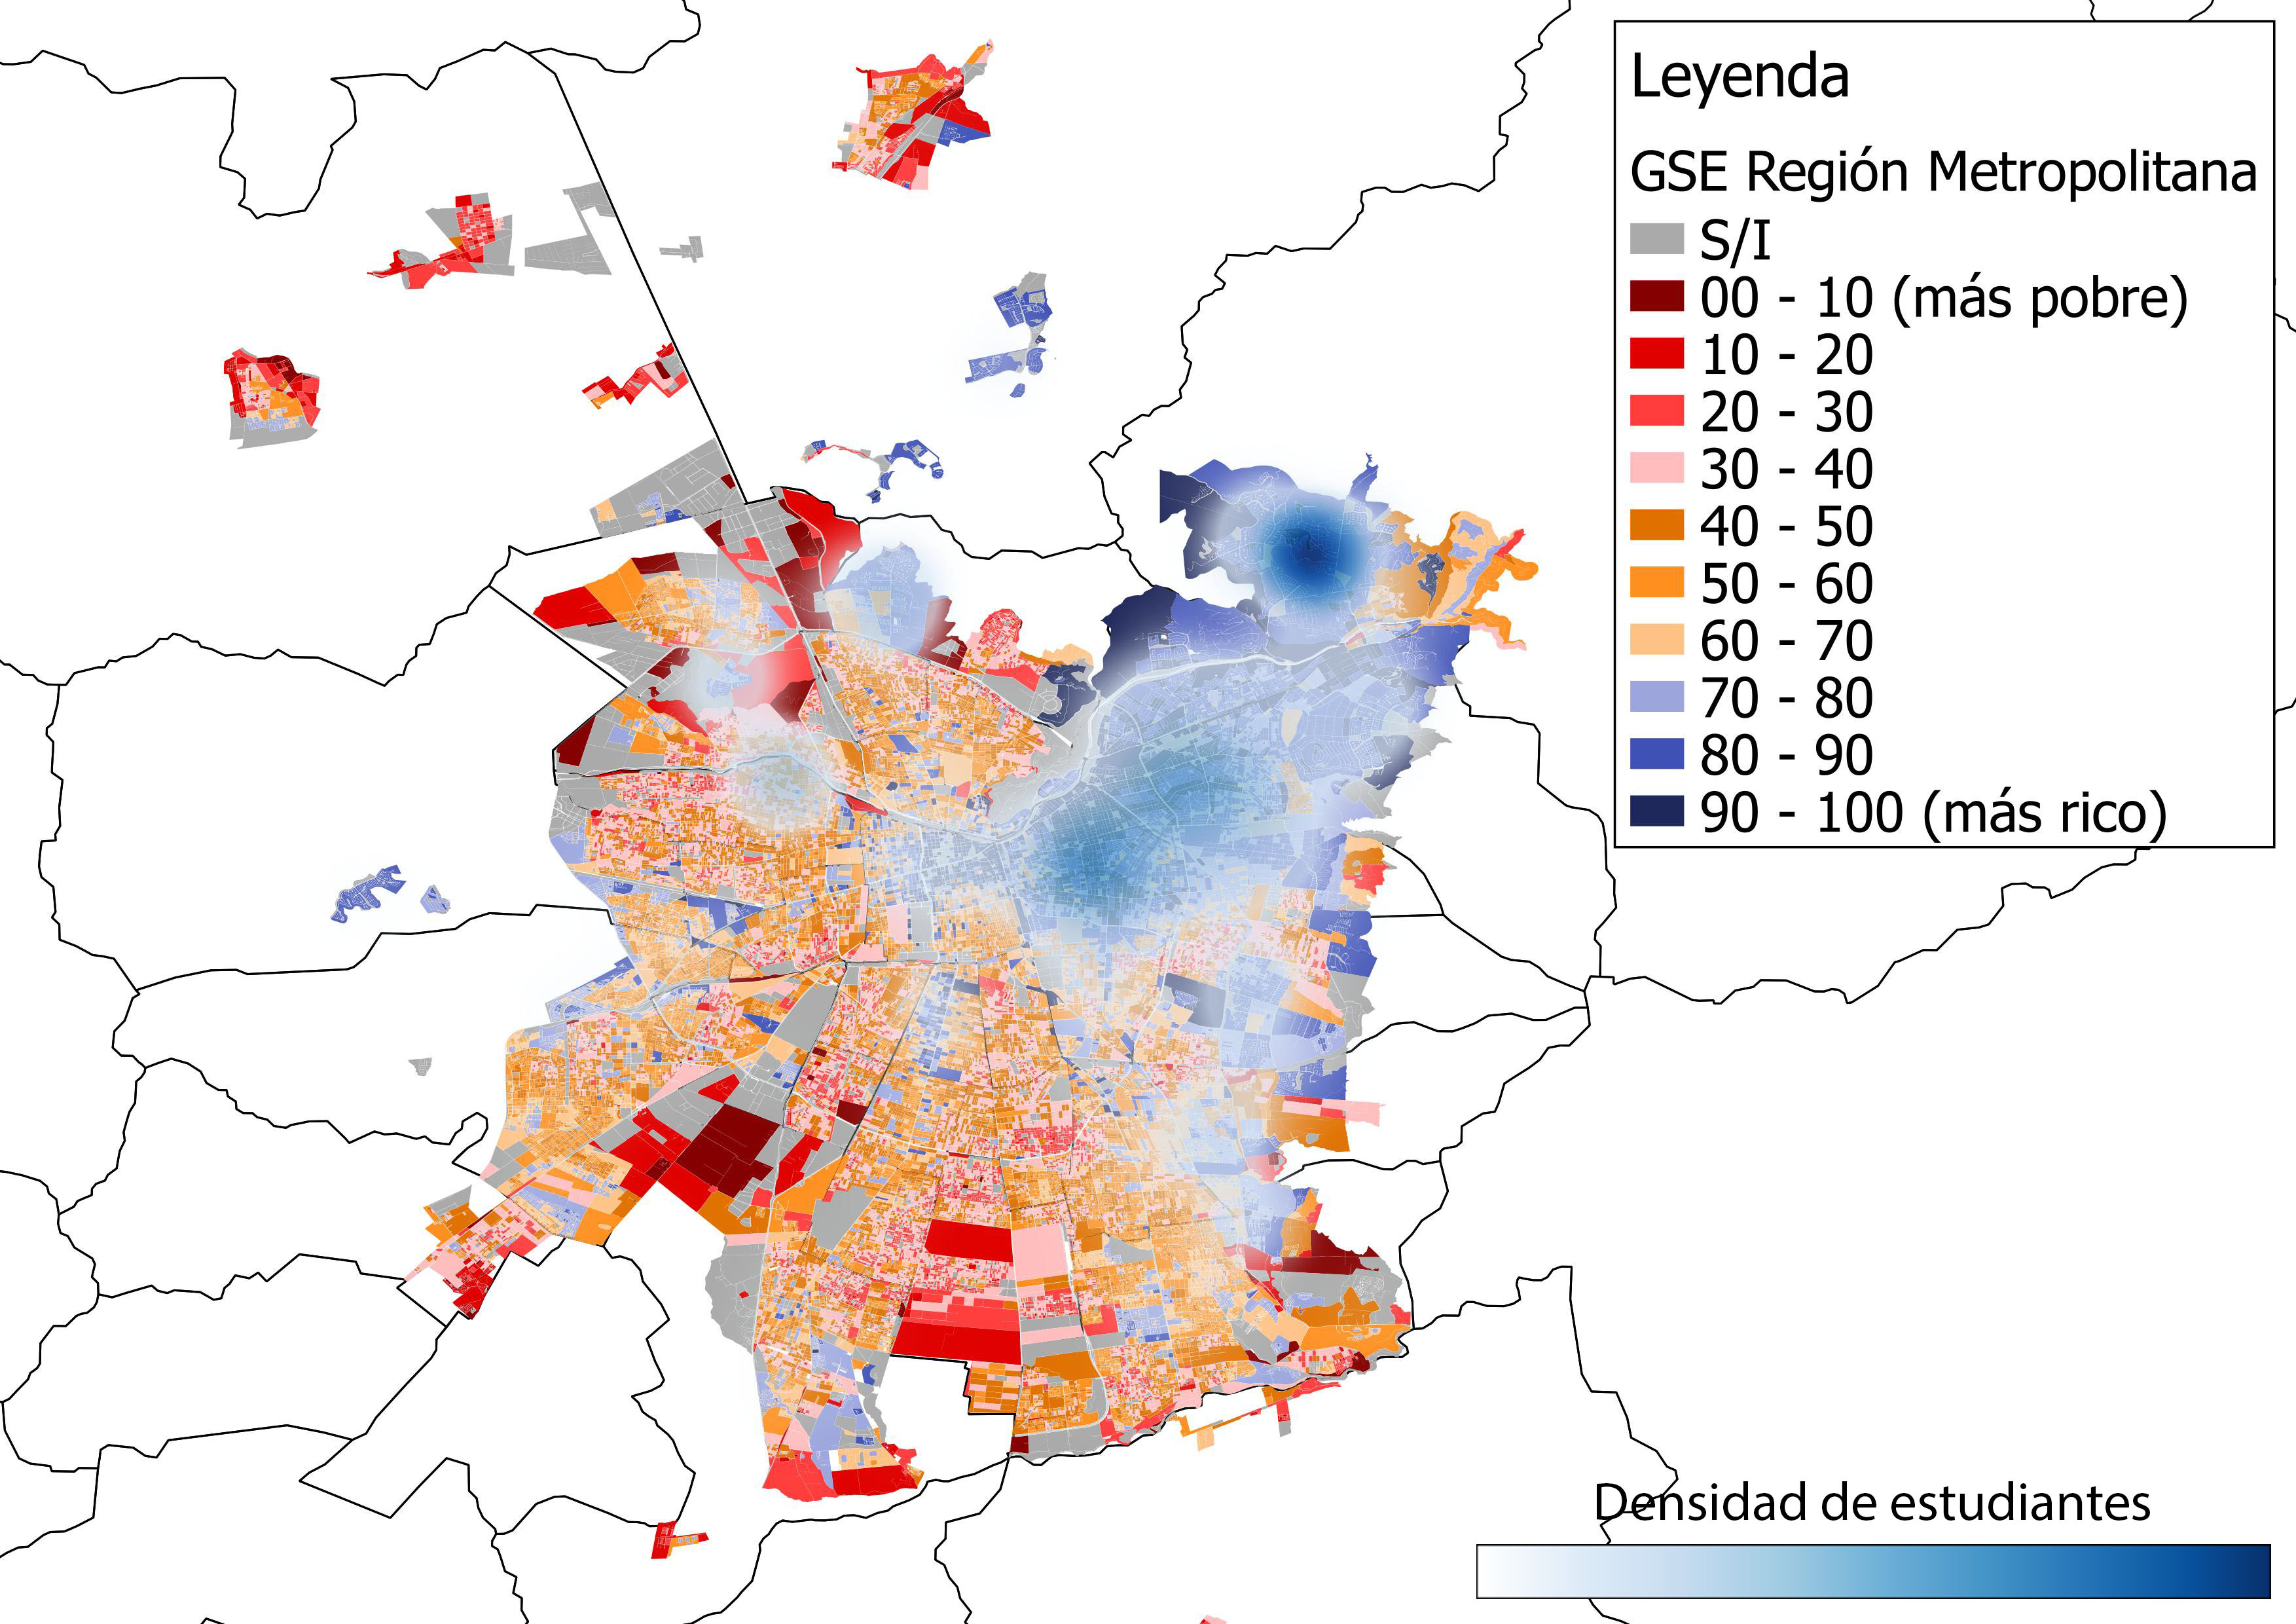
\includegraphics[width=7.5cm]{images/matriculas/E_CON_3_final.jpg}}
 \caption{Mapas de calor de matrículas (con atributos relacionales) en clústers de establecimientos sobre mapa GSE de la Región Metropolitana.}
 \label{f:mapas_mat_en_estab_con_gse}
\end{figure}

Al momento de analizar la distribución de los clúster de matrículas sin considerar los atributos de relación, podemos ver en la figura \ref{f:mapas_mat_sin_gse} que los clúster MCB y HCB se distribuyen de manera similar. Los estudiantes de dichos clústers están dispersos por casi toda el área metropolitana, disminuyendo su cantidad en el sector oriente y concentrándose en el sector sur y poniente. Por otro lado los clústers MSB y HSB se distribuyen de igual manera, ocupando toda el área metropolitana. Estos presentan varias zonas de alta densidad de alumnos, destacando entre ellas la zona norte del sector oriente de la capital.

Además, en las imágenes \ref{f:mapas_mat_sin_gse} se aprecian los grupos socioeconómicos en los cuales los clústers se encuentran, los primeros dos están presentes en los deciles del 4 al 7 principalmente y los otros dos en los deciles del 4 al 10, donde su \textit{peak} está en los deciles del 8 al 10.


\begin{figure}[H]
 \centering
  \subfloat[Matrículas clúster MCB.]{
   \label{f:mapa_mat_sin_0_gse}
    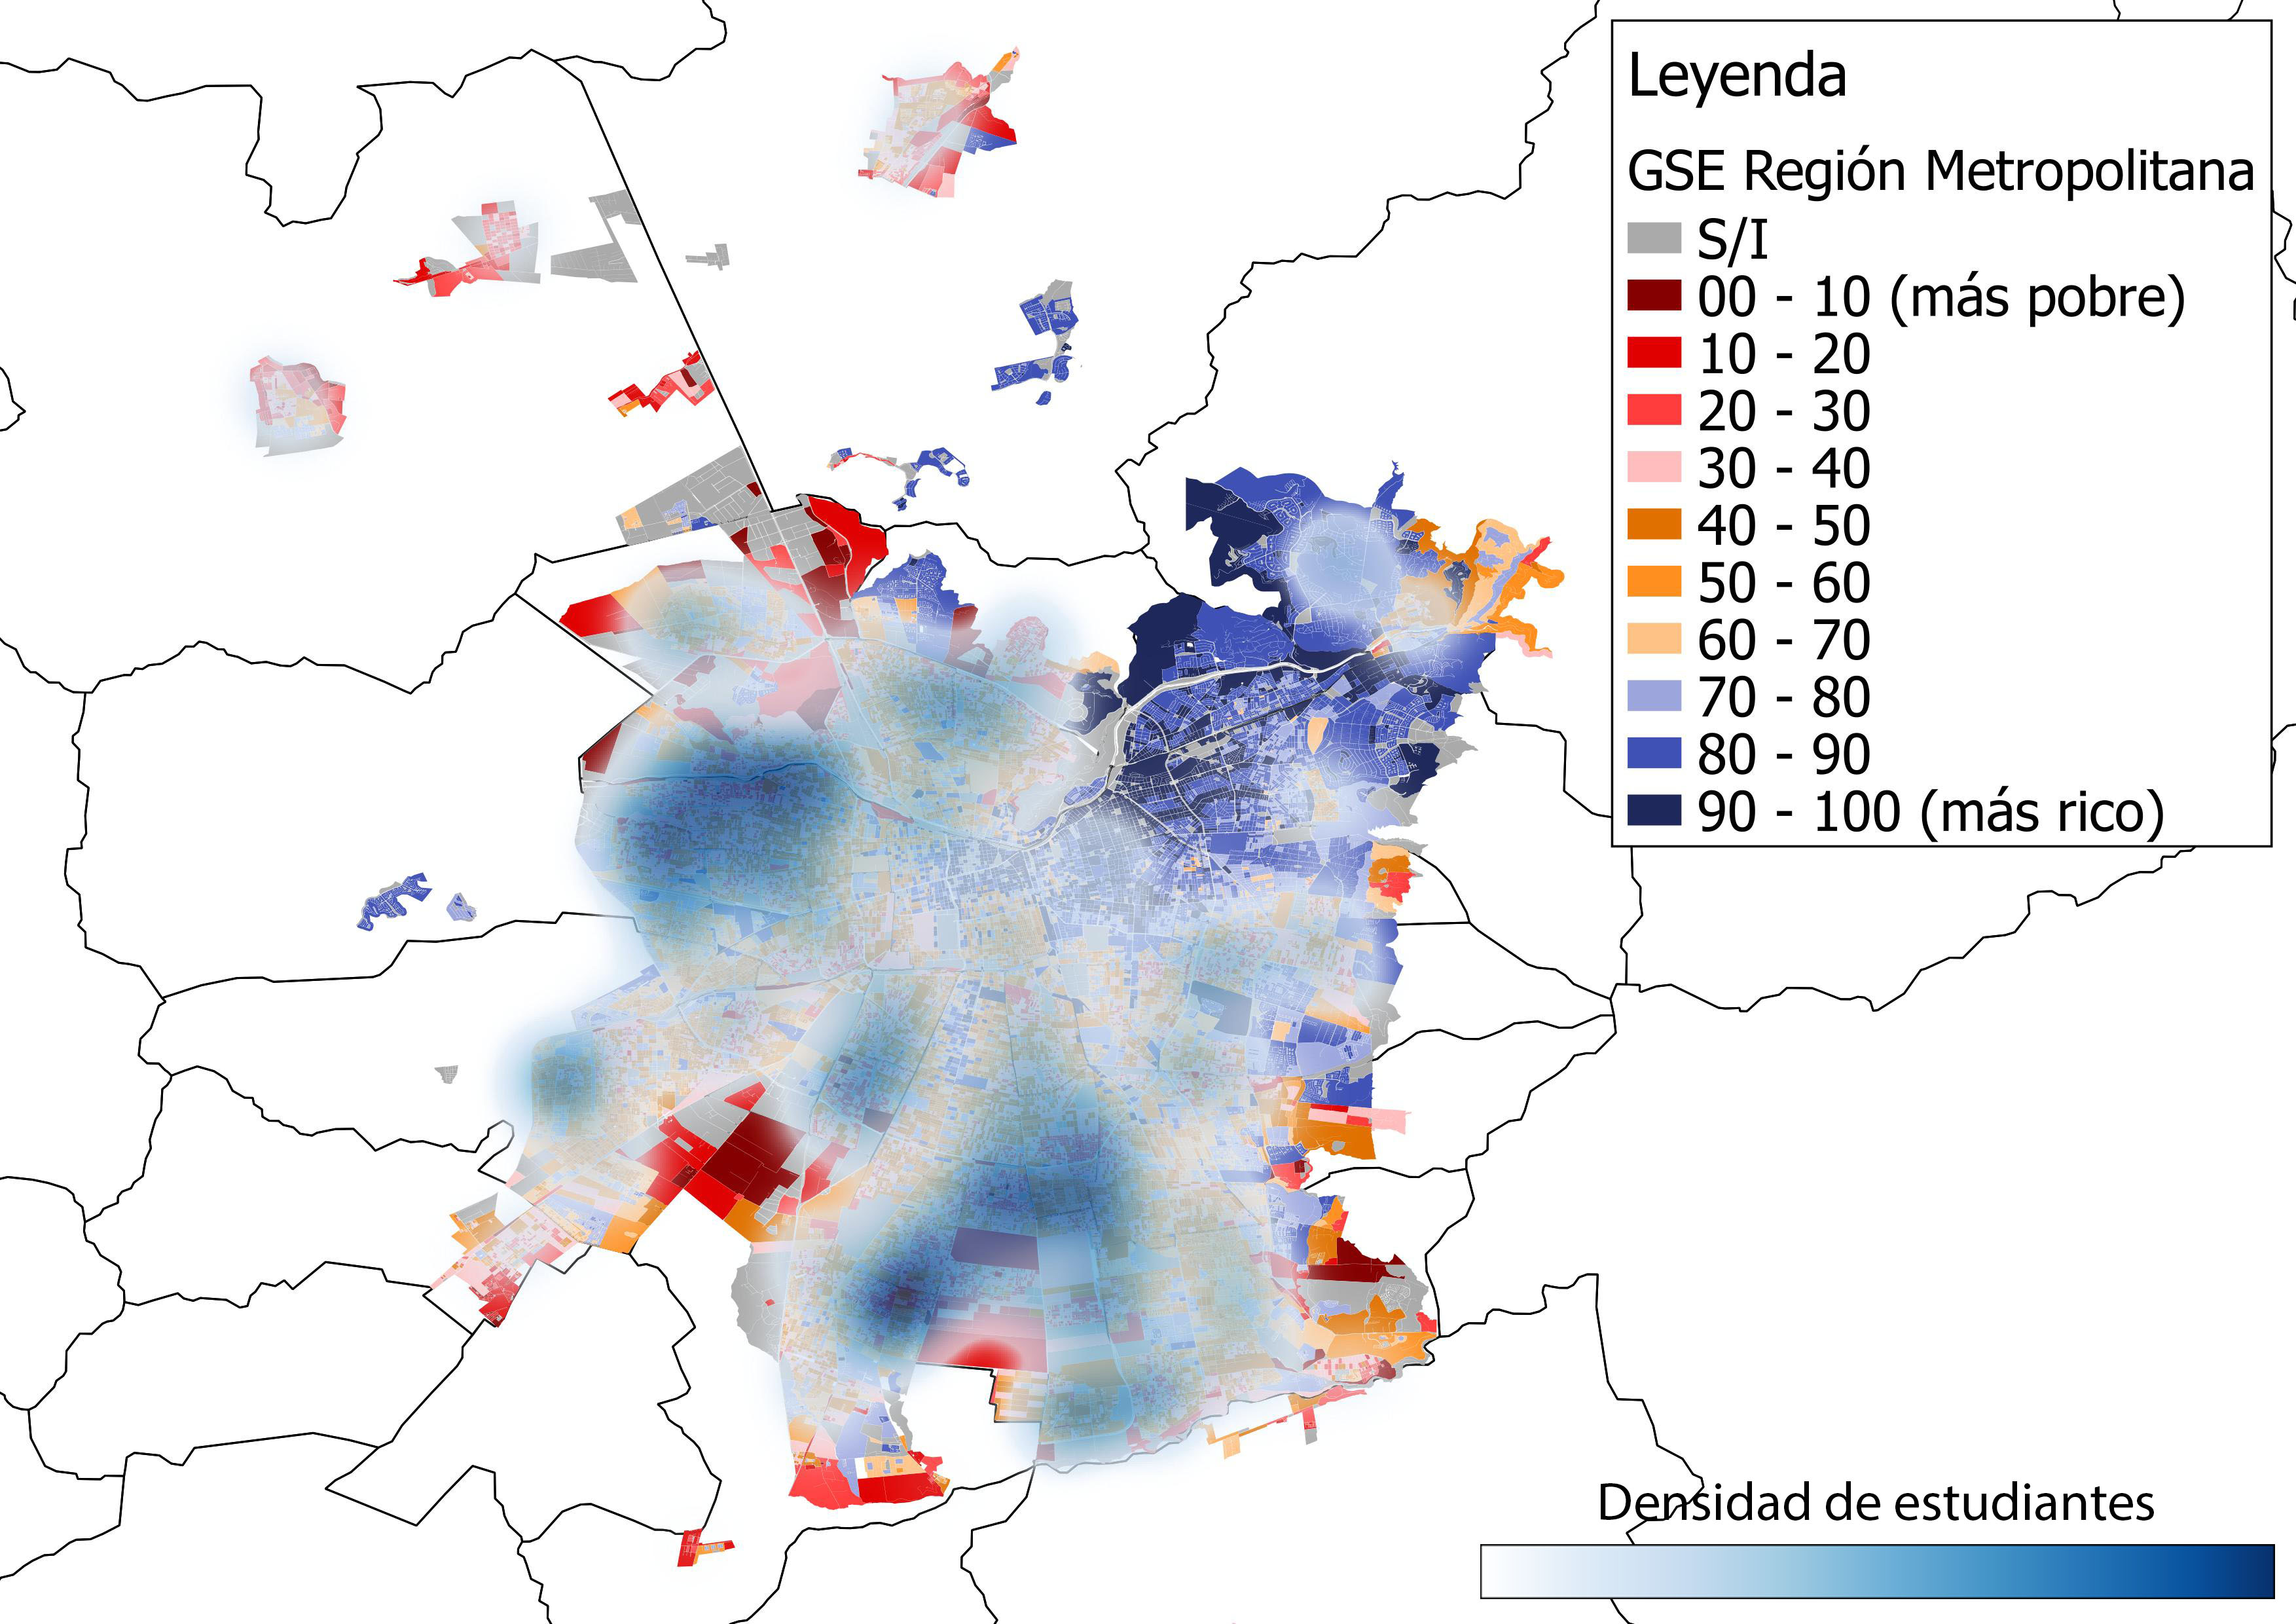
\includegraphics[width=7.5cm]{images/matriculas/M_SIN_0_final.jpg}}
  \subfloat[Matrículas clúster HCB.]{
   \label{f:mapa_mat_sin_1_gse}
    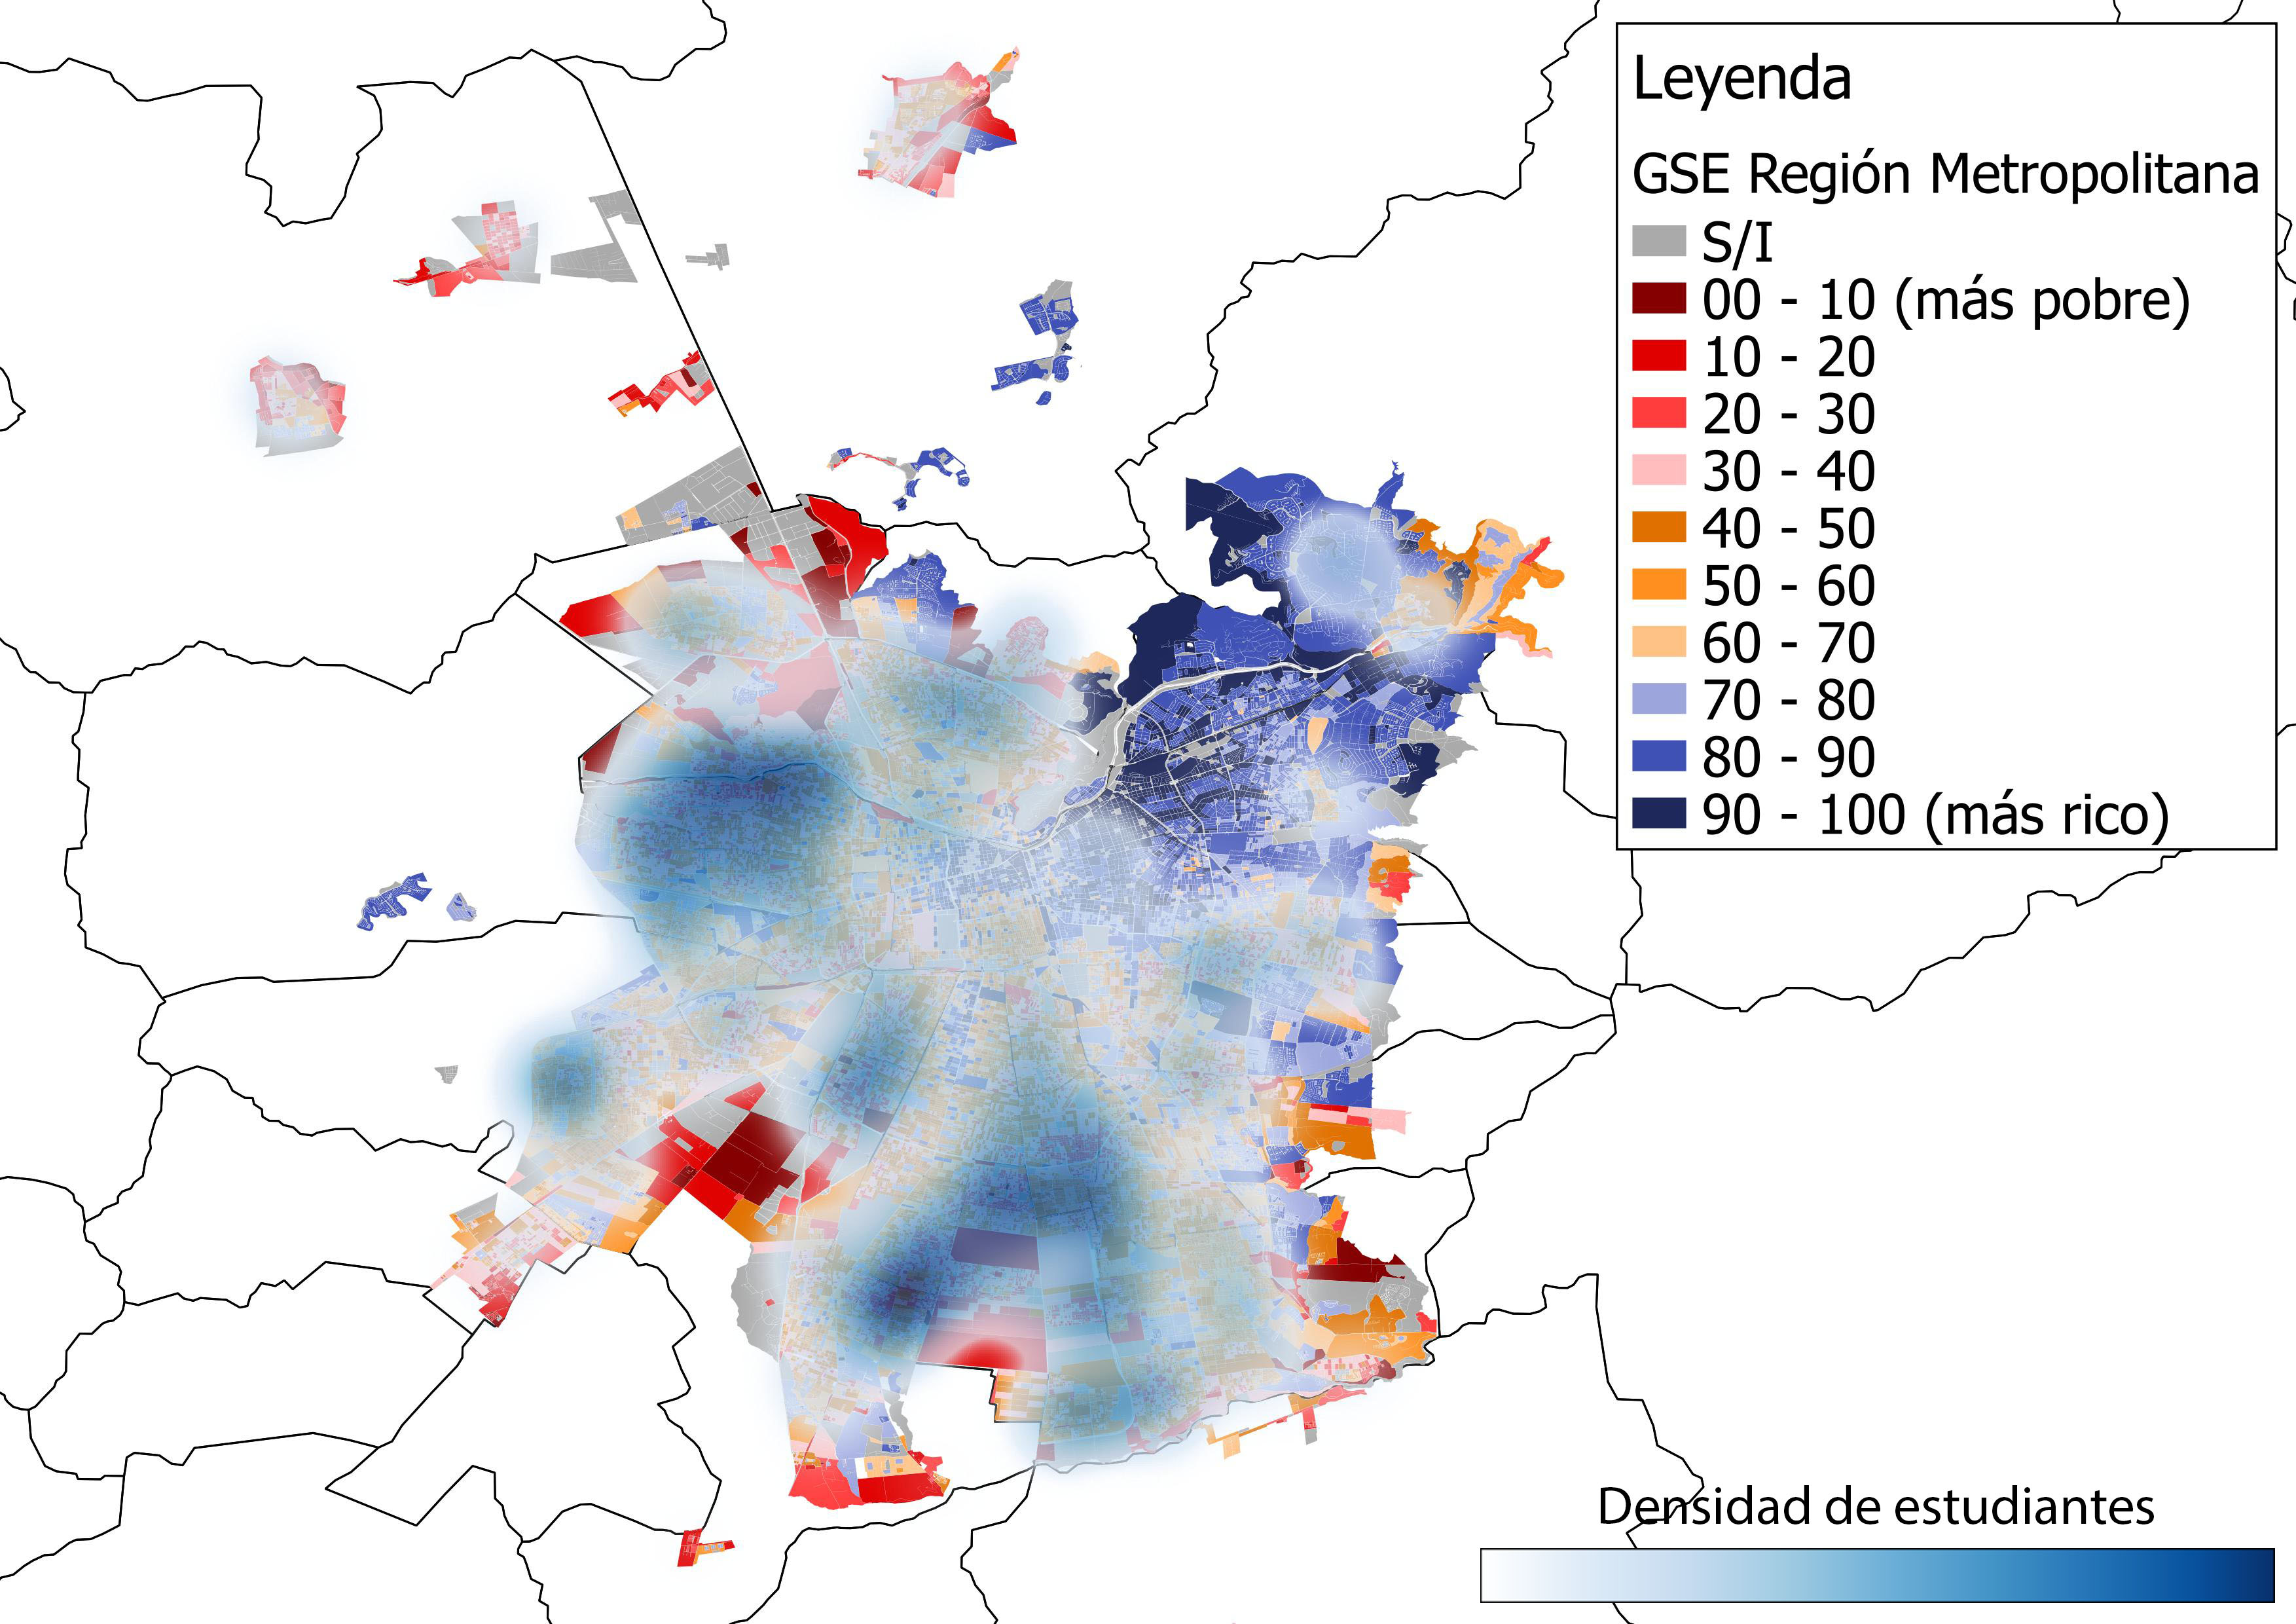
\includegraphics[width=7.5cm]{images/matriculas/M_SIN_1_final.jpg}}\hspace{1mm}
  \subfloat[Matrículas clúster MSB.]{
   \label{f:mapa_mat_sin_2_gse}
    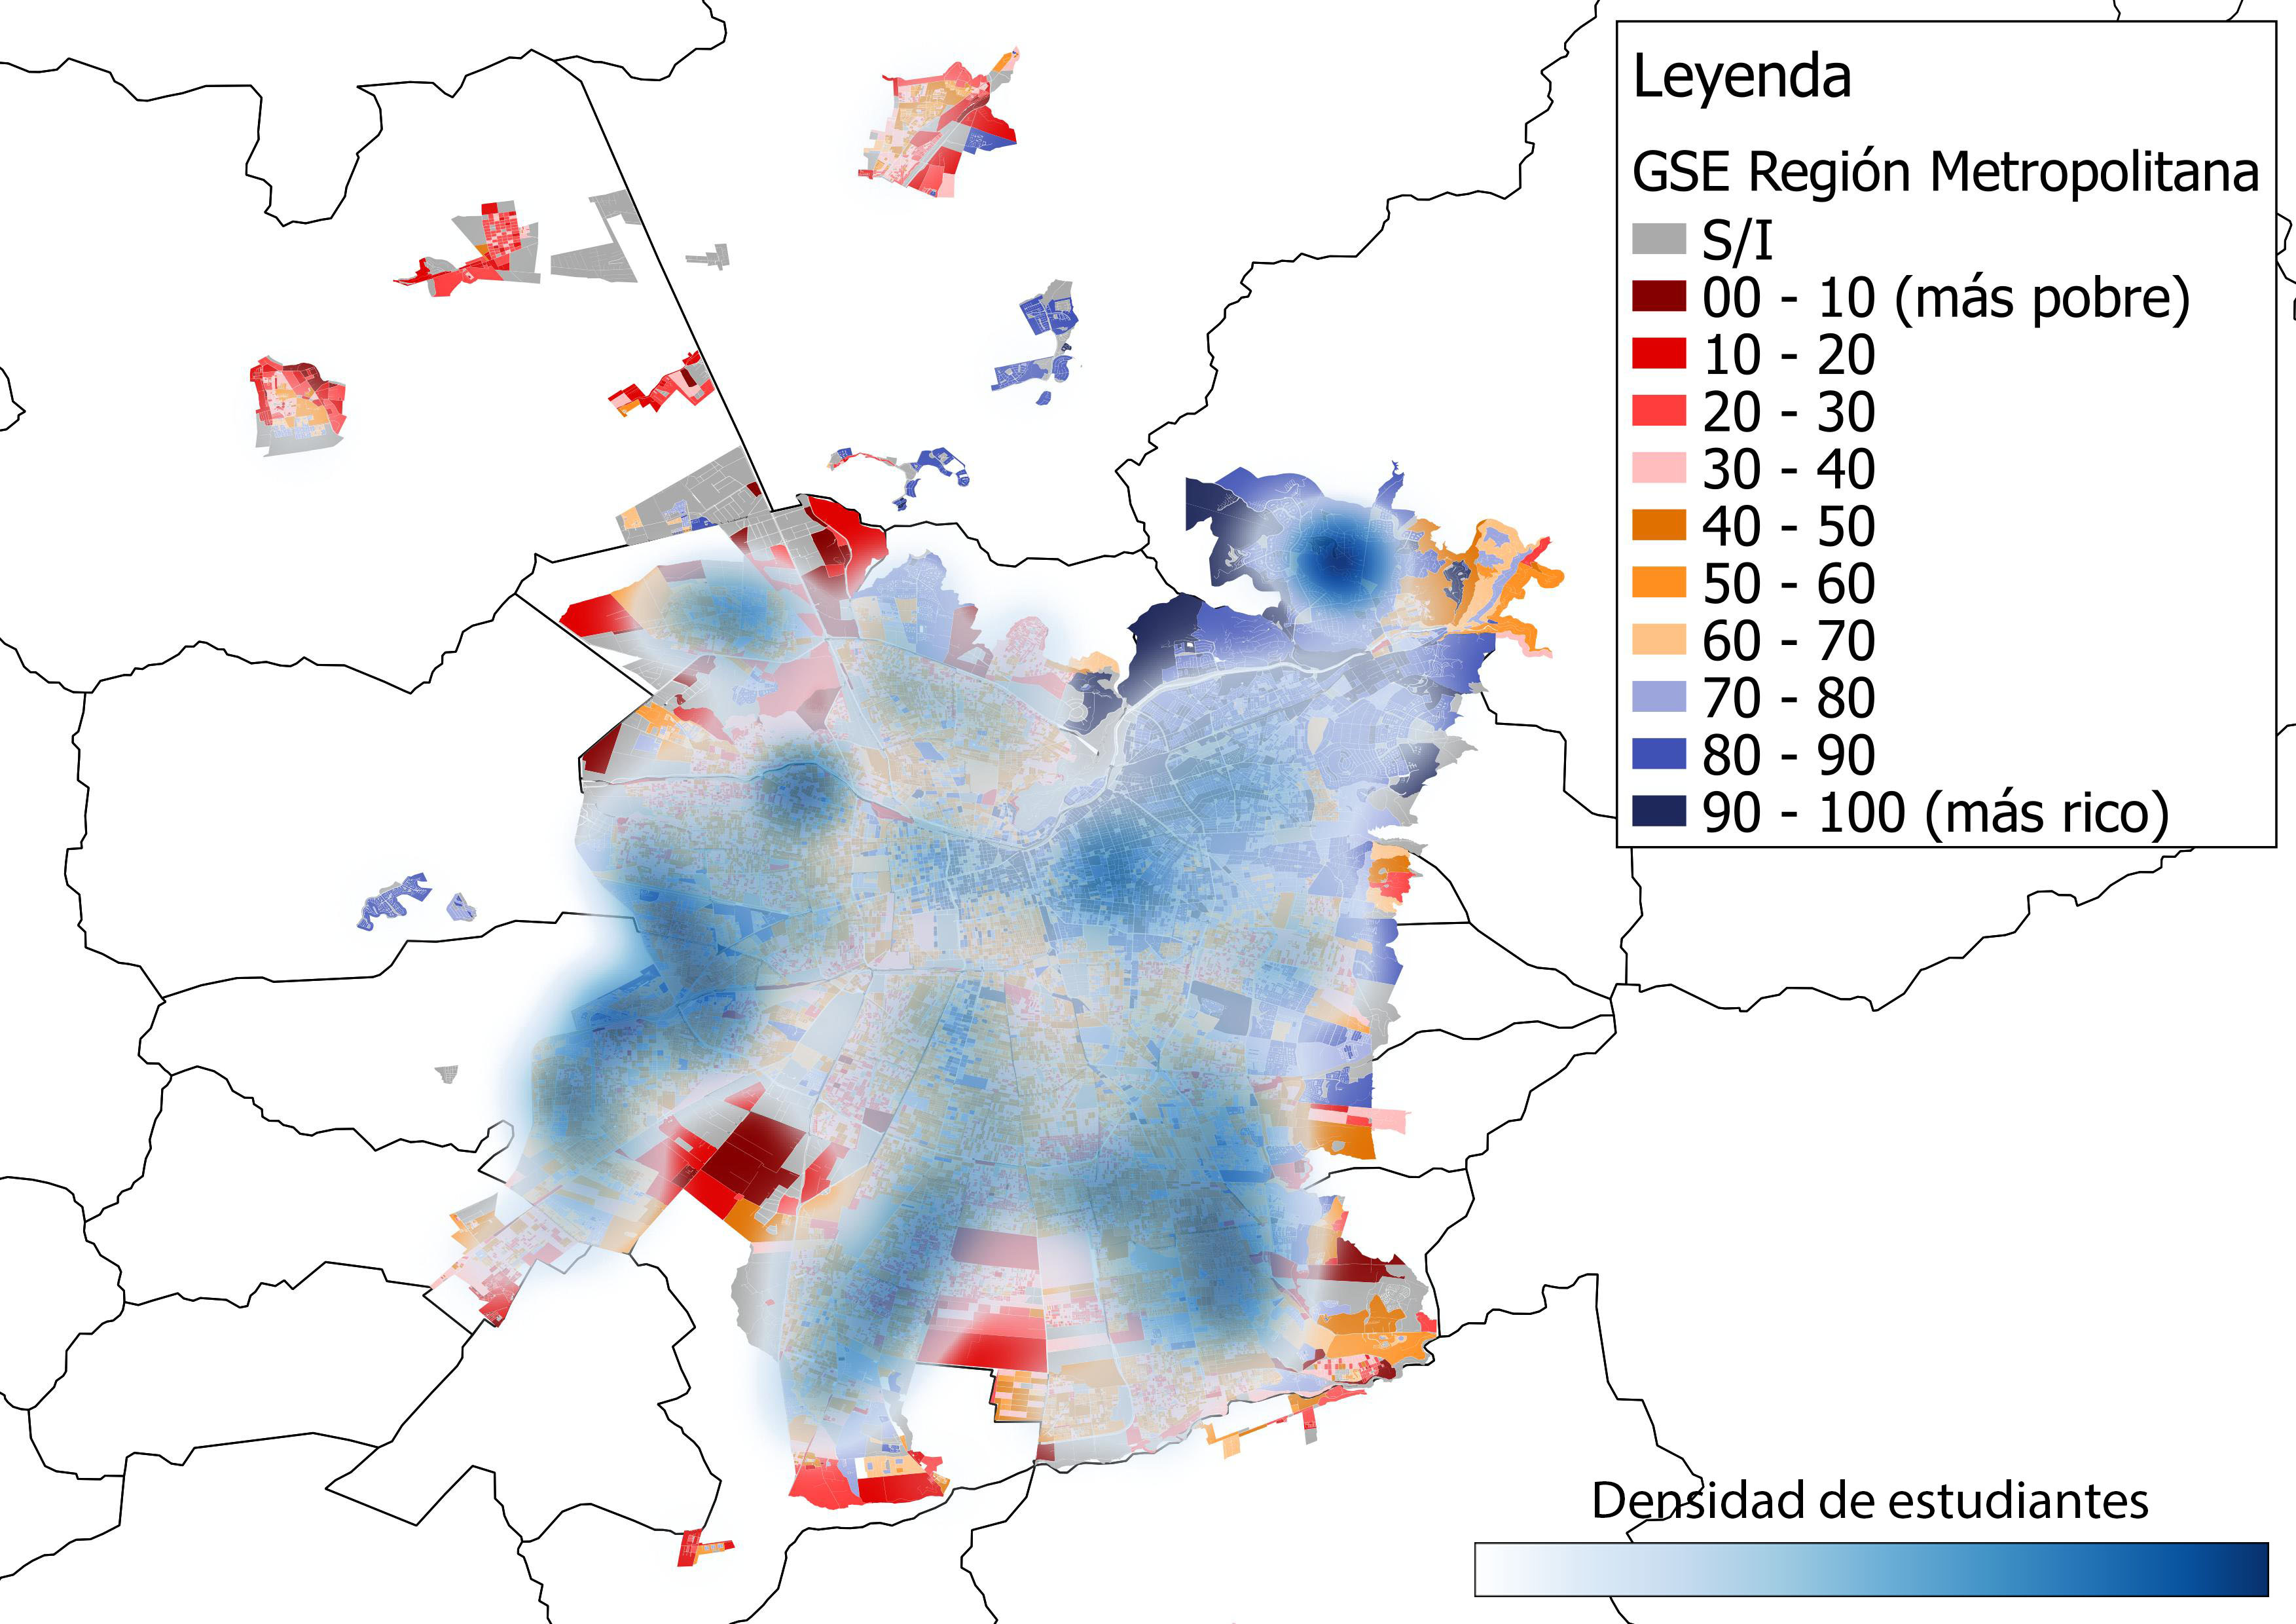
\includegraphics[width=7.5cm]{images/matriculas/M_SIN_2_final.jpg}}
  \subfloat[Matrículas clúster HSB.]{
   \label{f:mapa_mat_sin_3_gse}
    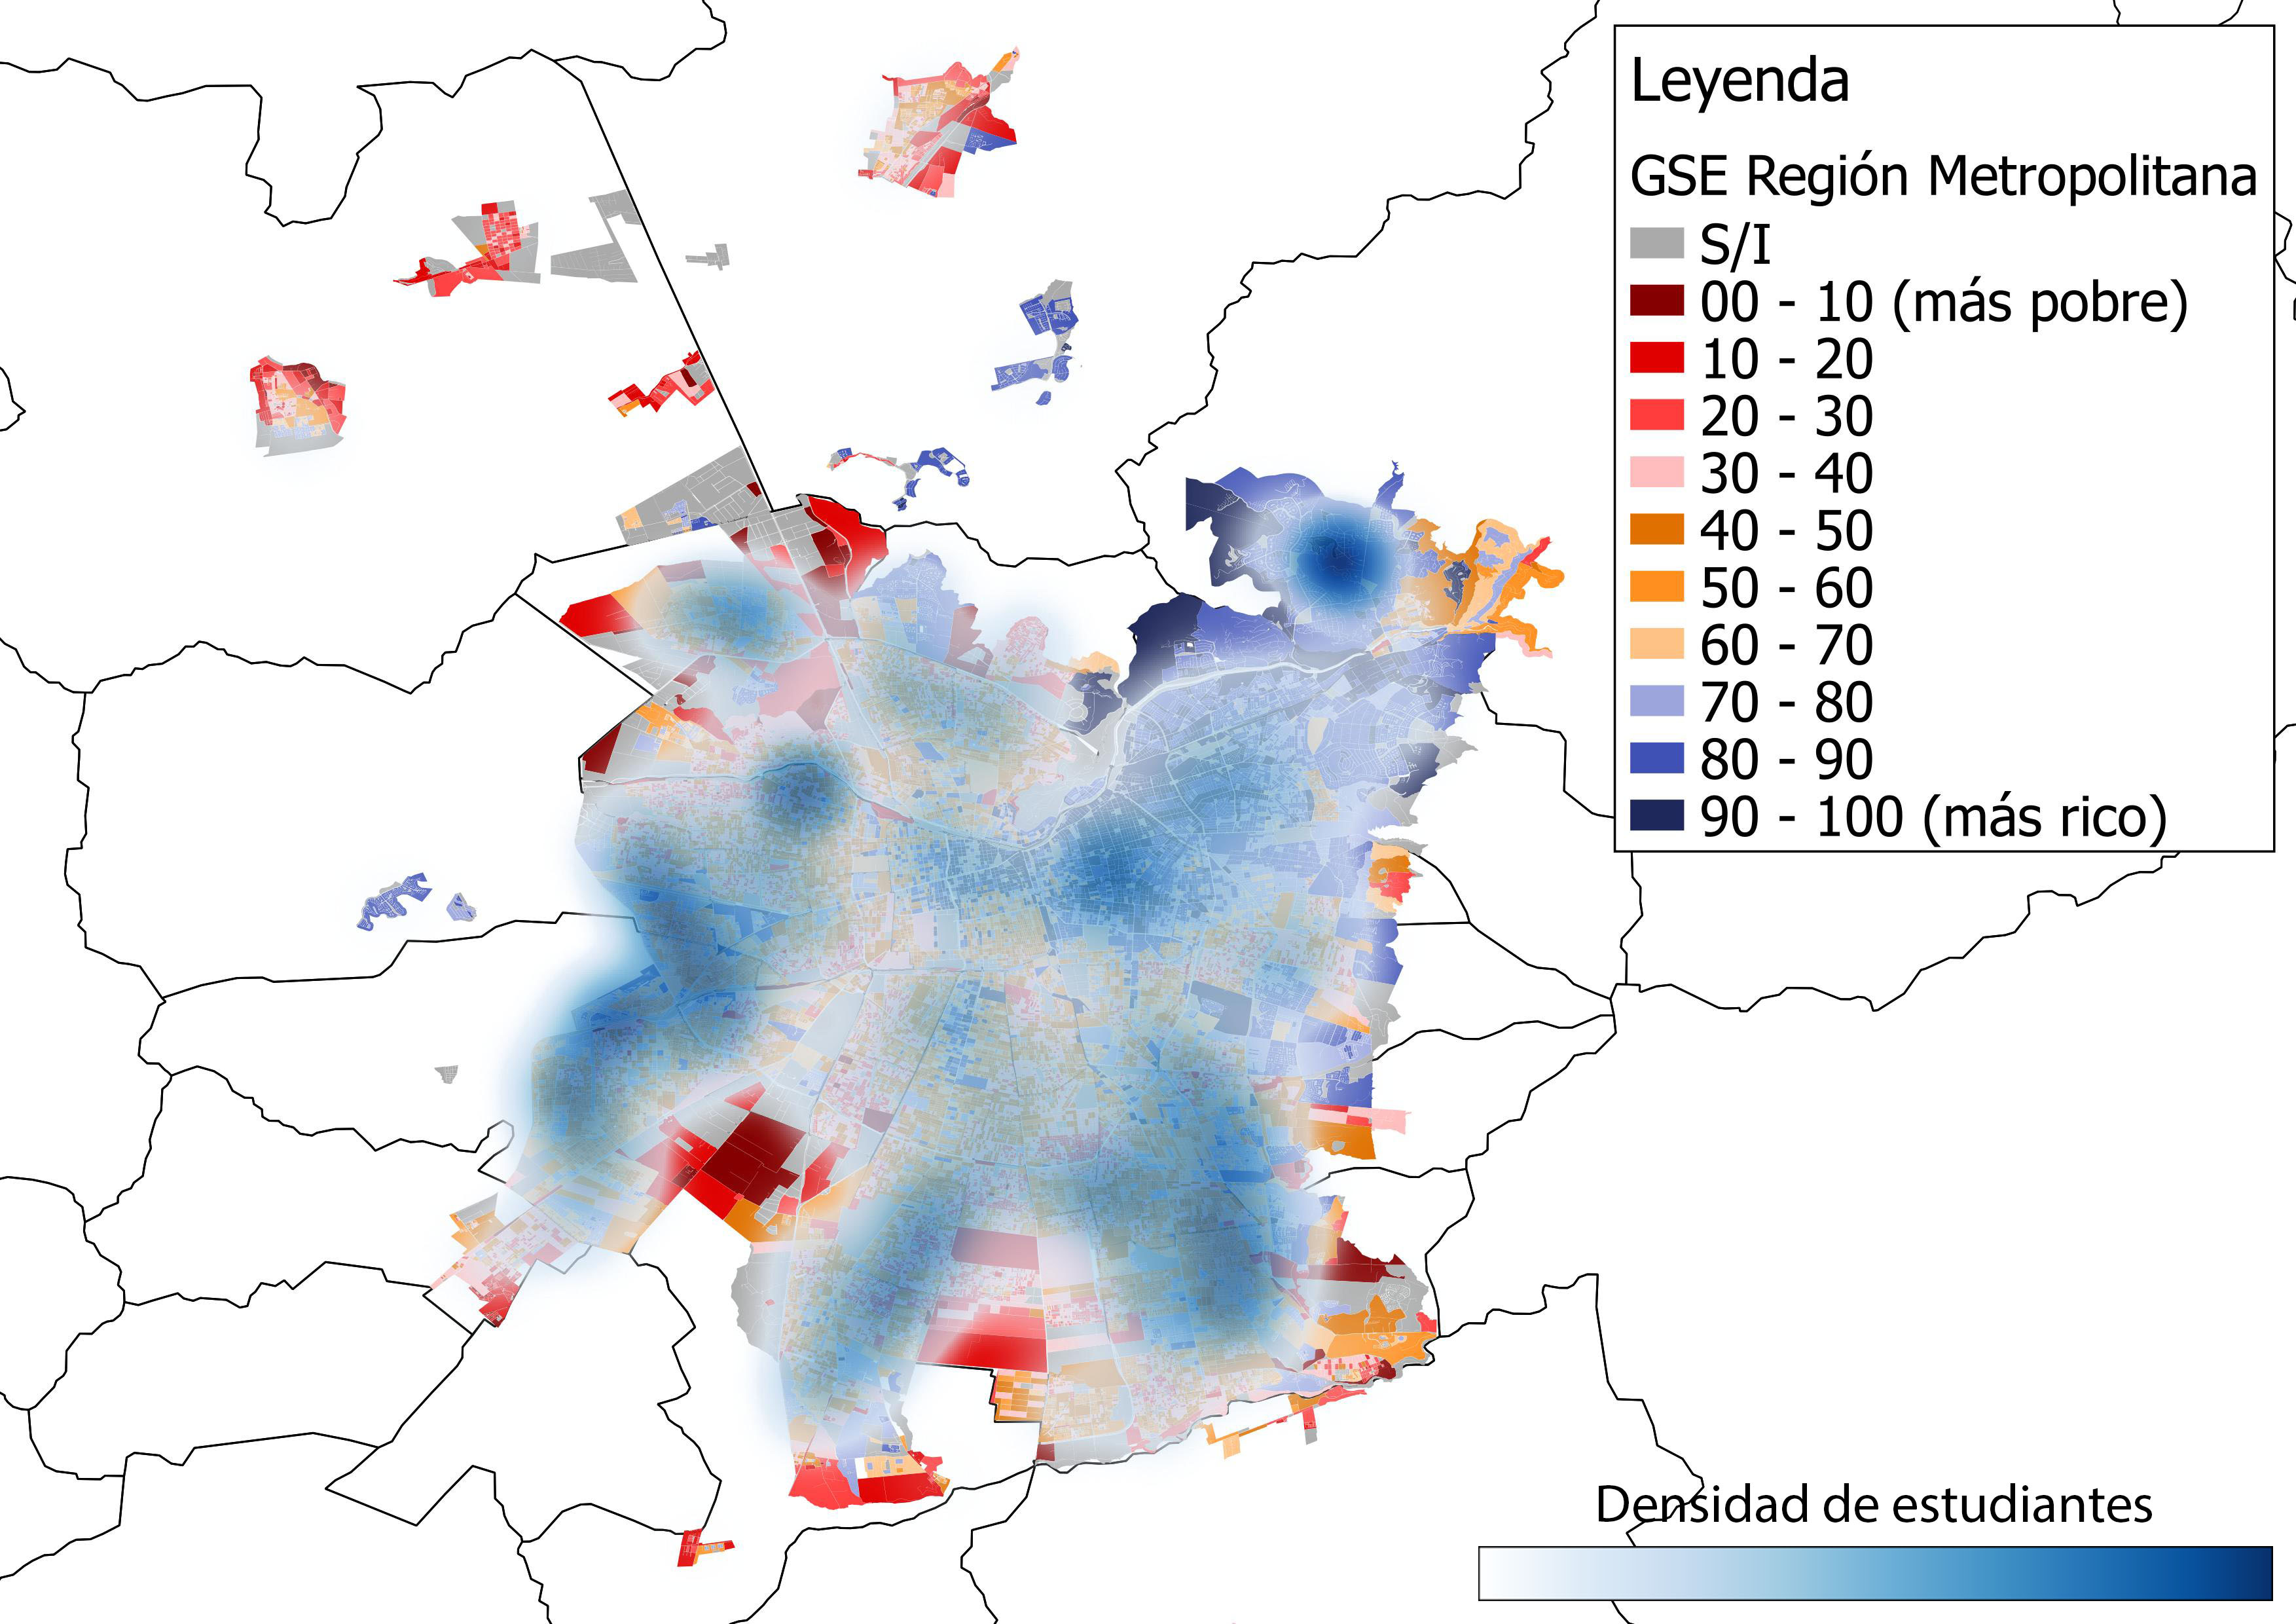
\includegraphics[width=7.5cm]{images/matriculas/M_SIN_3_final.jpg}}
 \caption{Mapas de calor de clústers de matrículas sobre mapa GSE de la Región Metropolitana.}
 \label{f:mapas_mat_sin_gse}
\end{figure}

Al analizar las imágenes \ref{f:mapa_mat_con_0_gse} y \ref{f:mapa_mat_con_1_gse} podemos observar una gran similitud, en donde los alumnos se distribuyen por casi toda el área metropolitana, pero disminuye notoriamente en el sector oriente. En la figura \ref{f:mapa_mat_con_2_gse} encontramos alumnos en casi toda la capital, pero se concentran en 3 sectores,  2 en la zona sur y 1 en la zona poniente. Por último, en \ref{f:mapa_mat_con_3_gse}, casi todos los alumnos residen en el sector oriente de la capital, siendo la periferia de este donde existe una mayor concentración.

A diferencia del análisis sin variables de relación, las primeras 3 figuras muestran que los alumnos viven en sectores socioeconómicos que van del decil 2 al decil 8, es decir, comprenden grupos muy variados. Caso aparte es la última imagen, donde los estudiantes residen en sectores pertenecientes a los deciles del 8 al 10.

Un punto importante a destacar en ambos análisis de clústers de matrículas es que en general los alumnos no residen en sectores pertenecientes a lo deciles 1 y 2, es decir, a los sectores de menor ingreso.

\begin{figure}[H]
 \centering
  \subfloat[Matrículas clúster MCBBC.]{
   \label{f:mapa_mat_con_0_gse}
    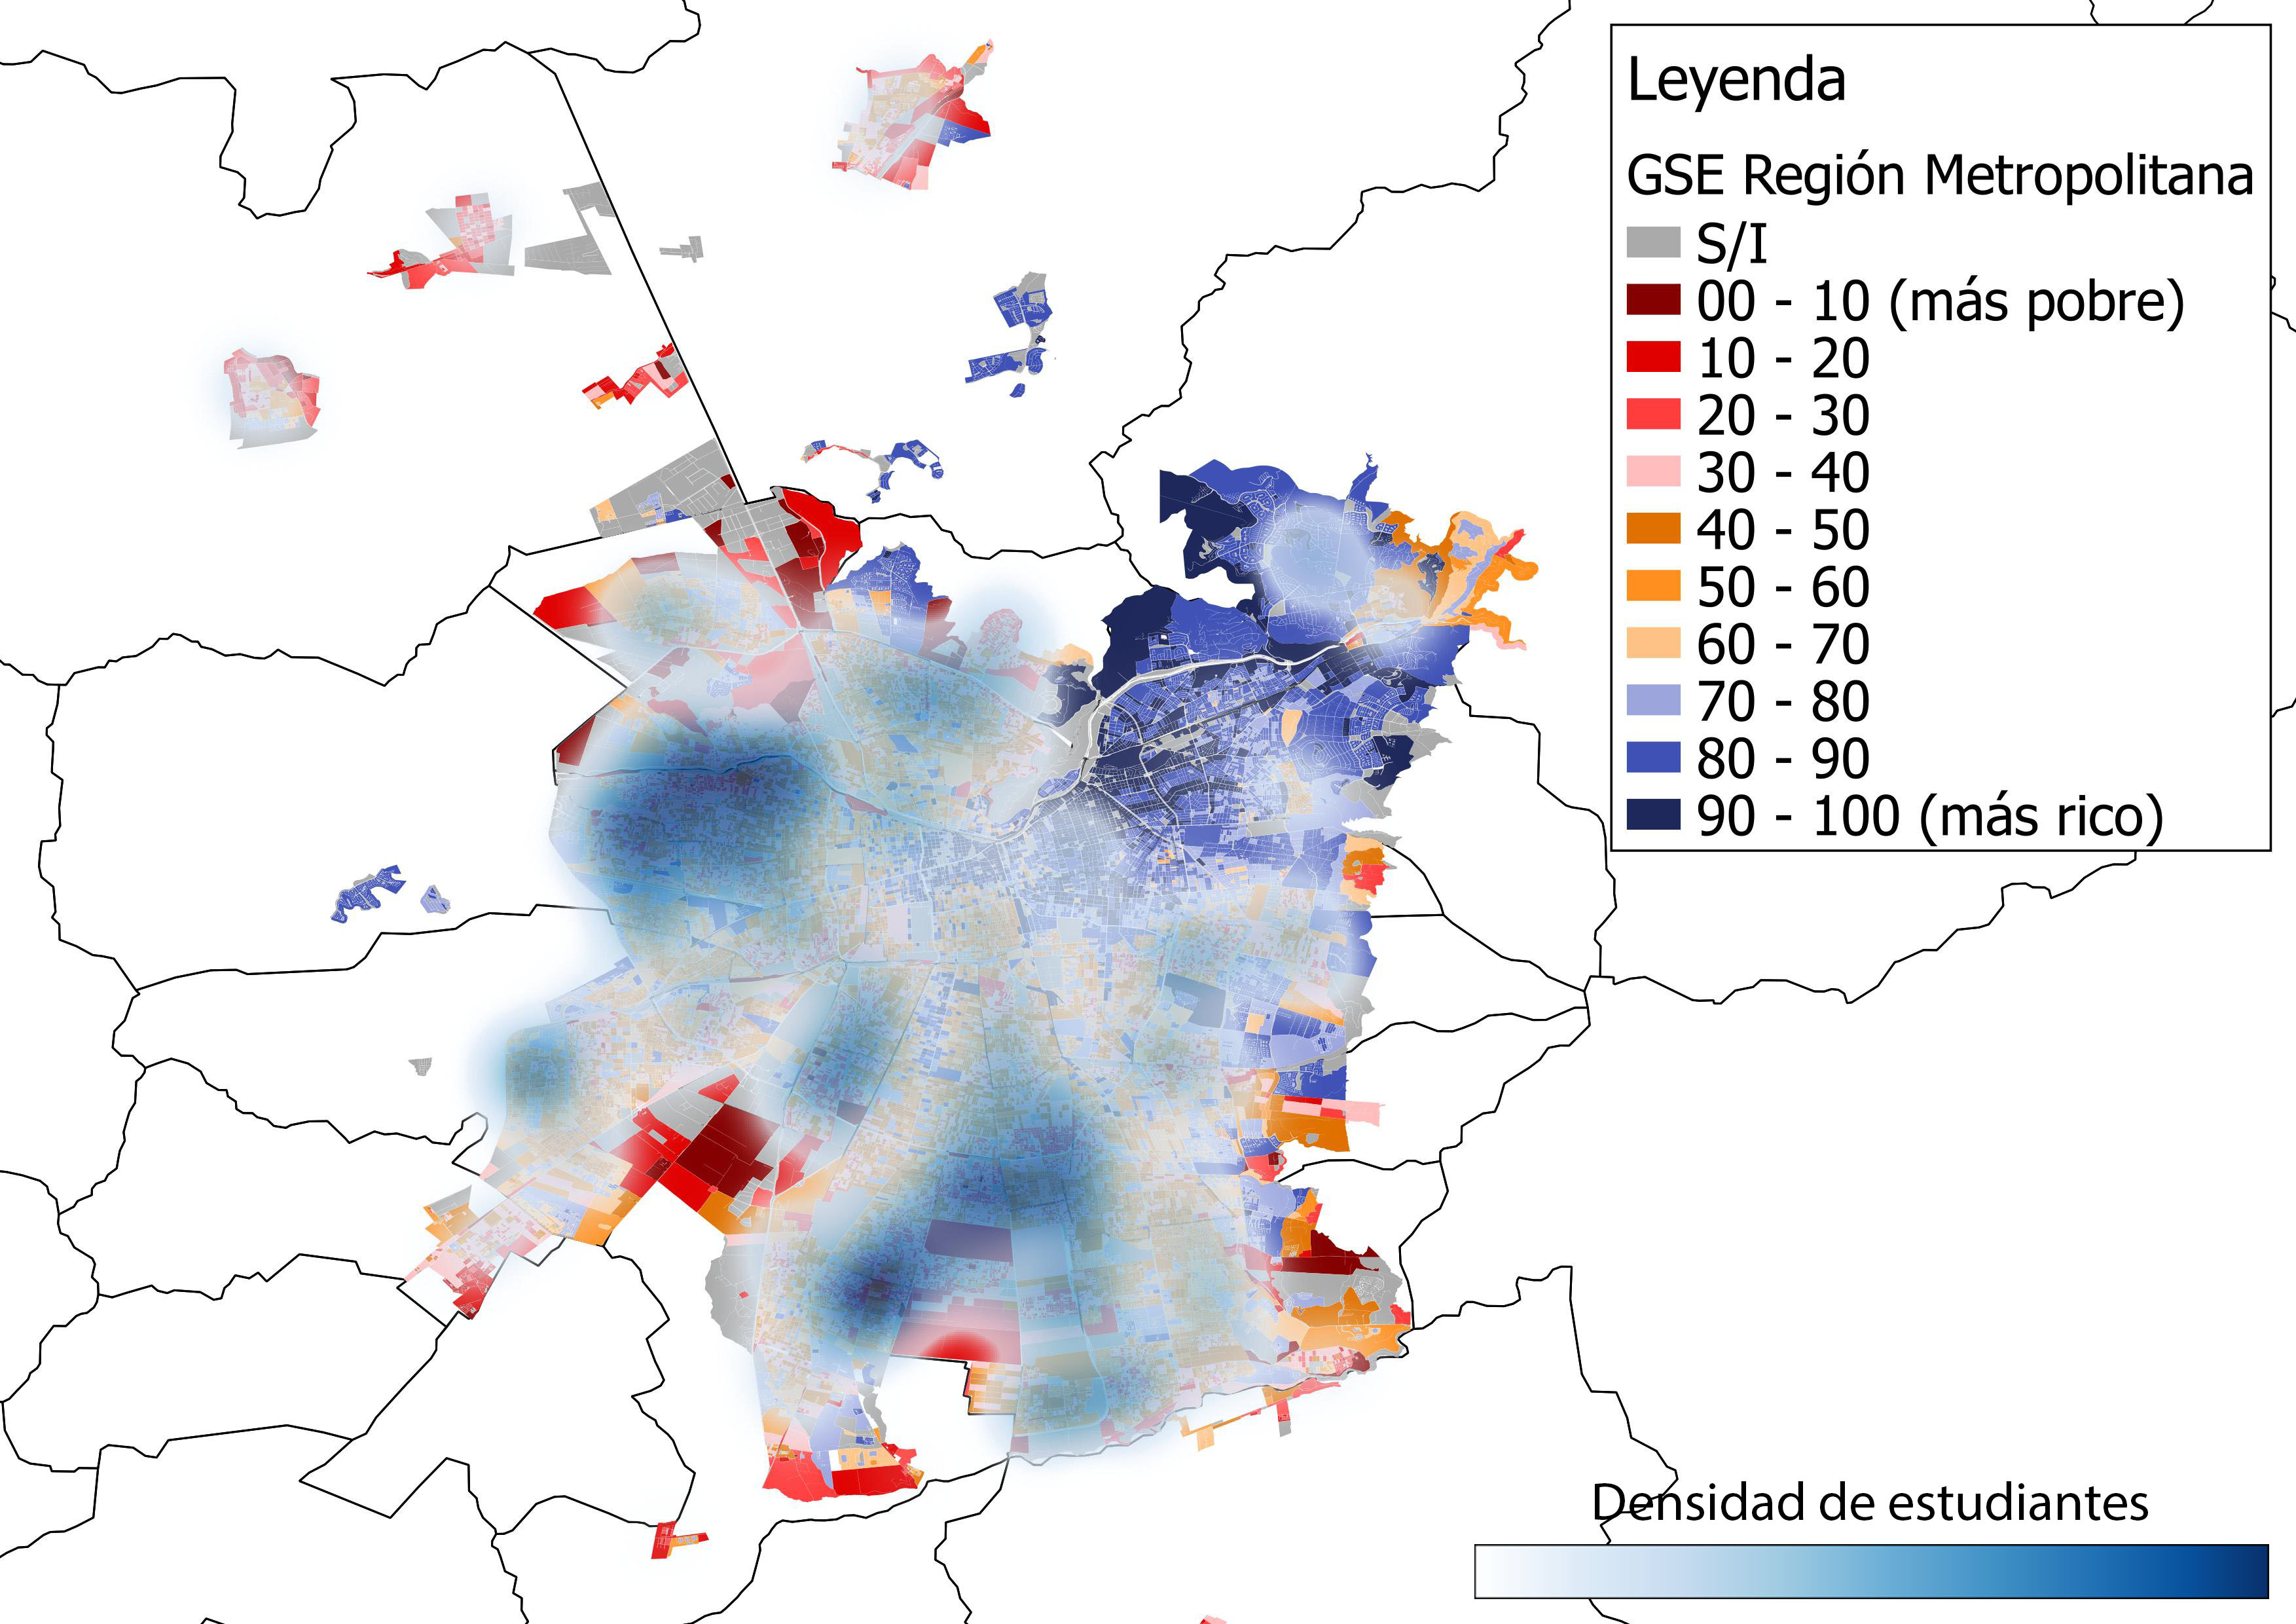
\includegraphics[width=7.5cm]{images/matriculas/M_CON_1_final.jpg}}
  \subfloat[Matrículas clúster HCBBC.]{
   \label{f:mapa_mat_con_1_gse}
    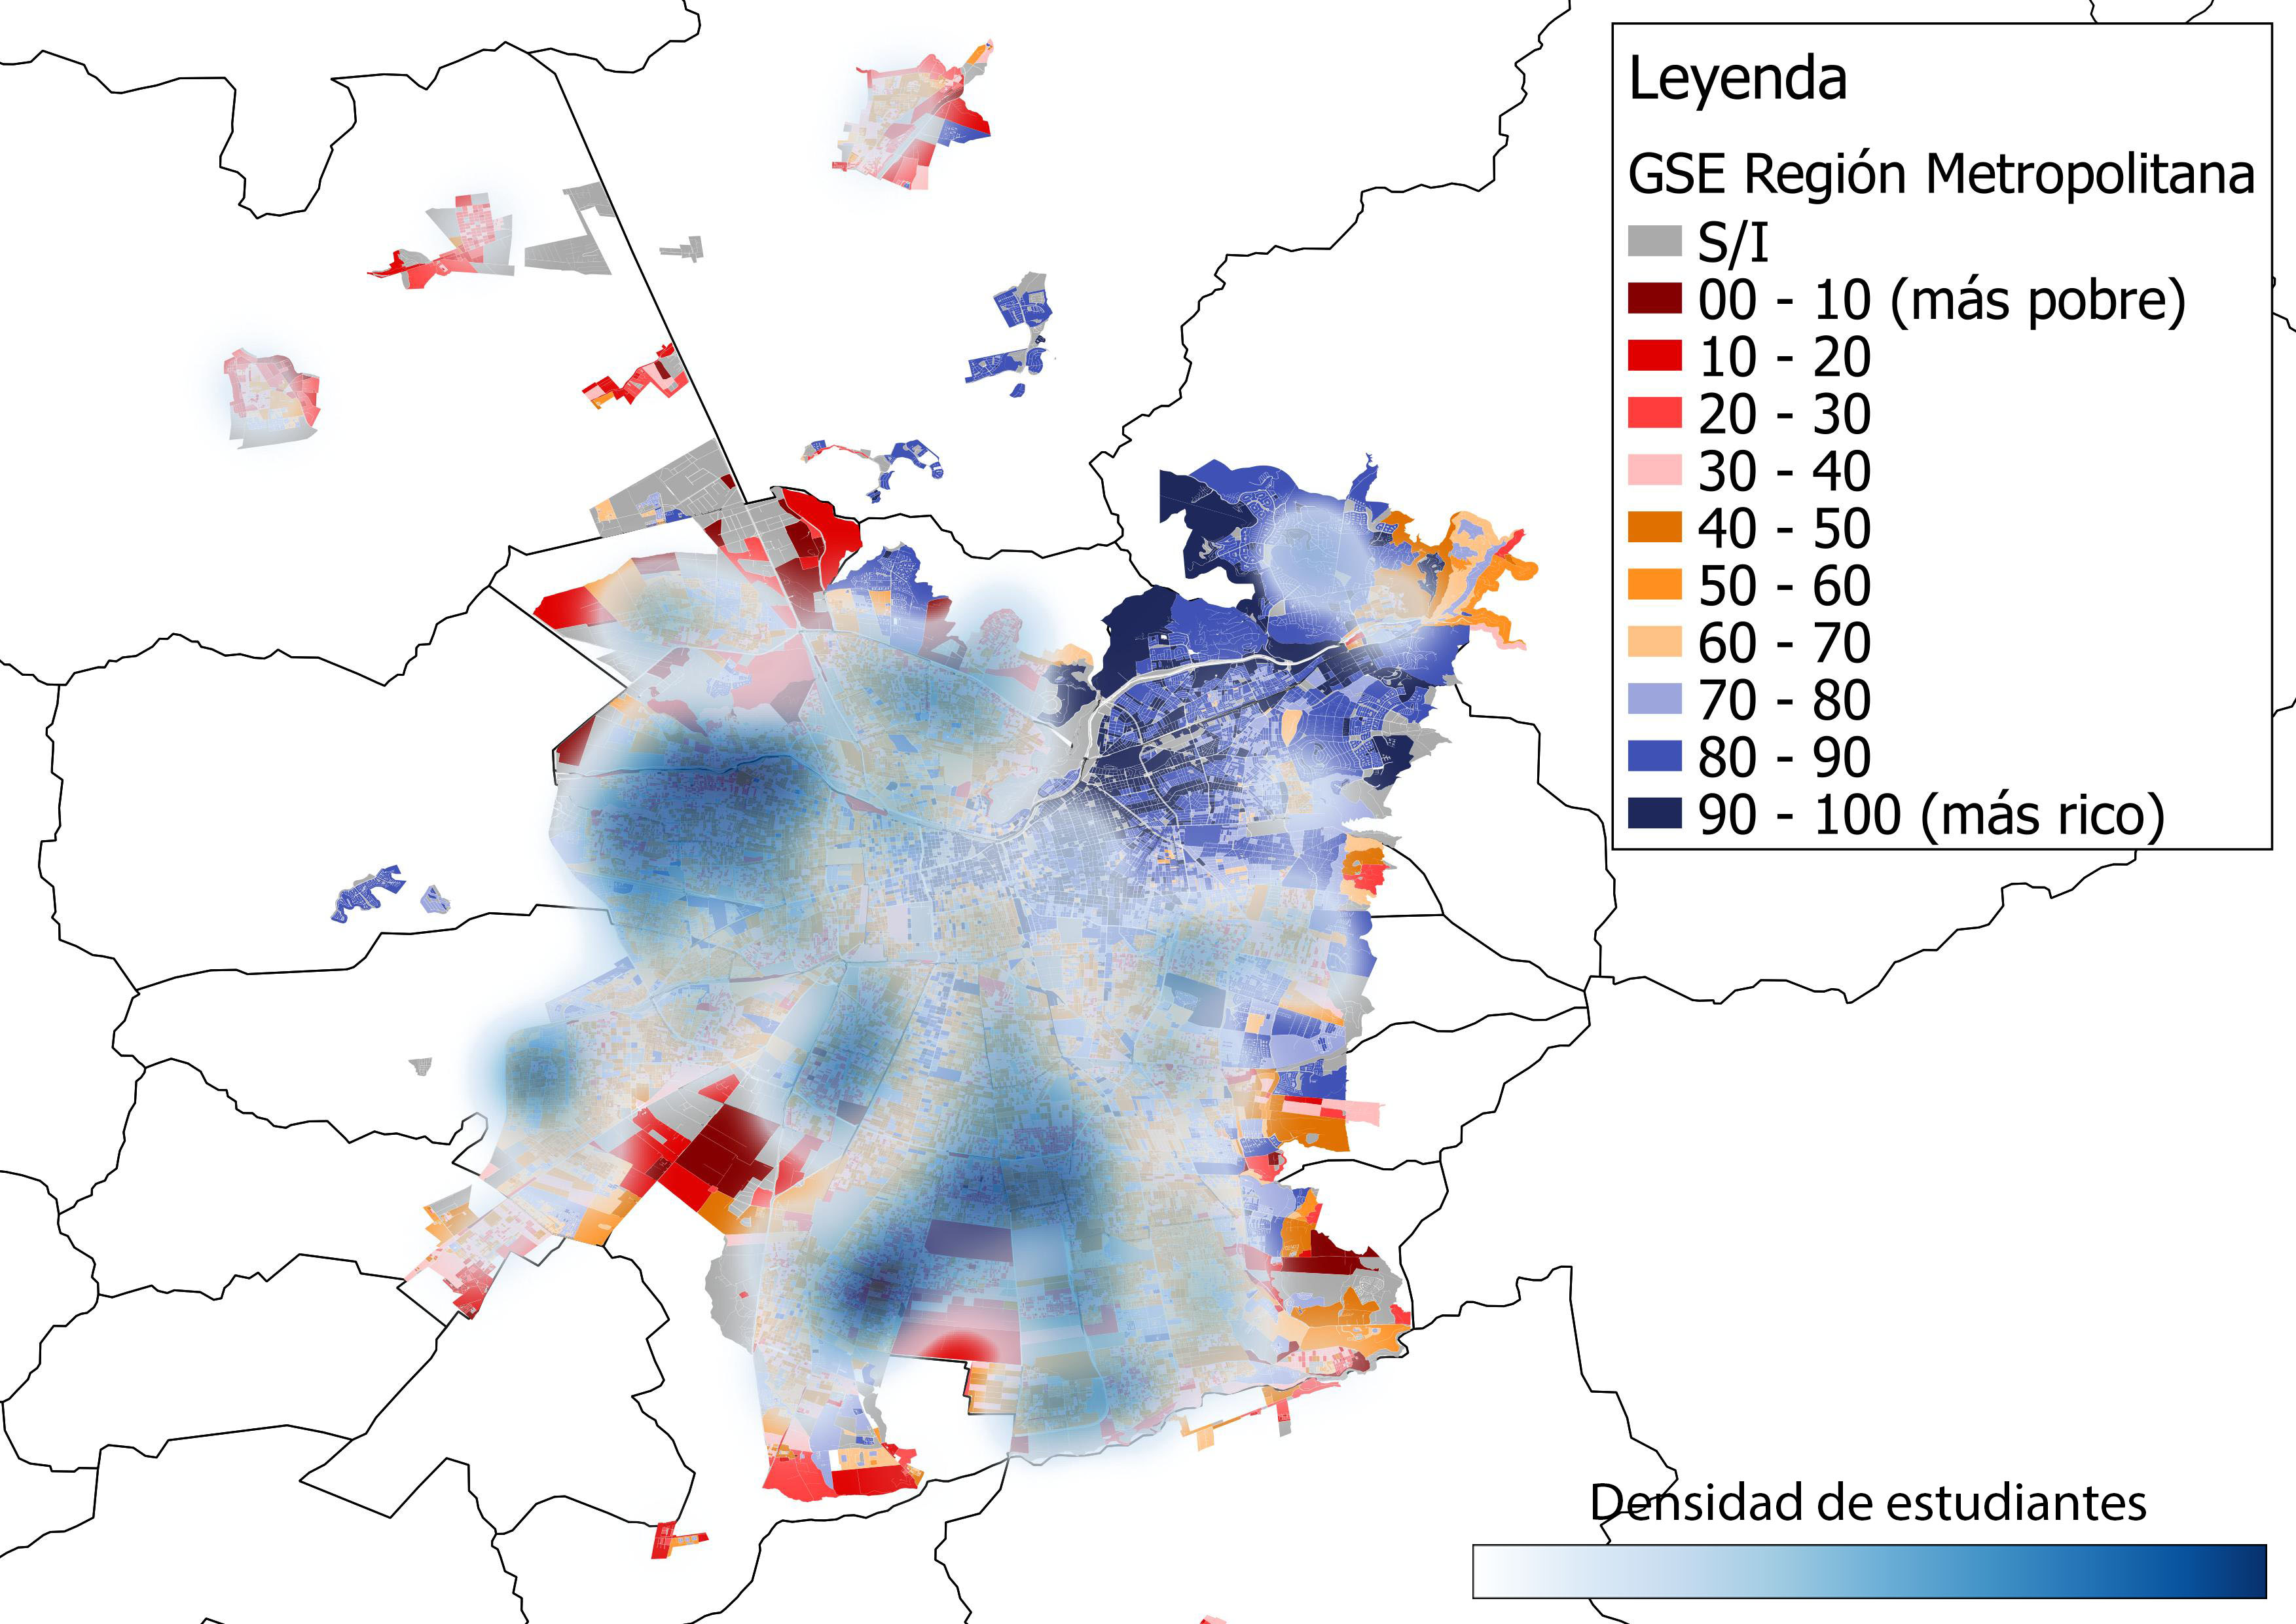
\includegraphics[width=7.5cm]{images/matriculas/M_CON_0_final.jpg}}\hspace{1mm}
  \subfloat[Matrículas clúster MiSBMC.]{
   \label{f:mapa_mat_con_2_gse}
    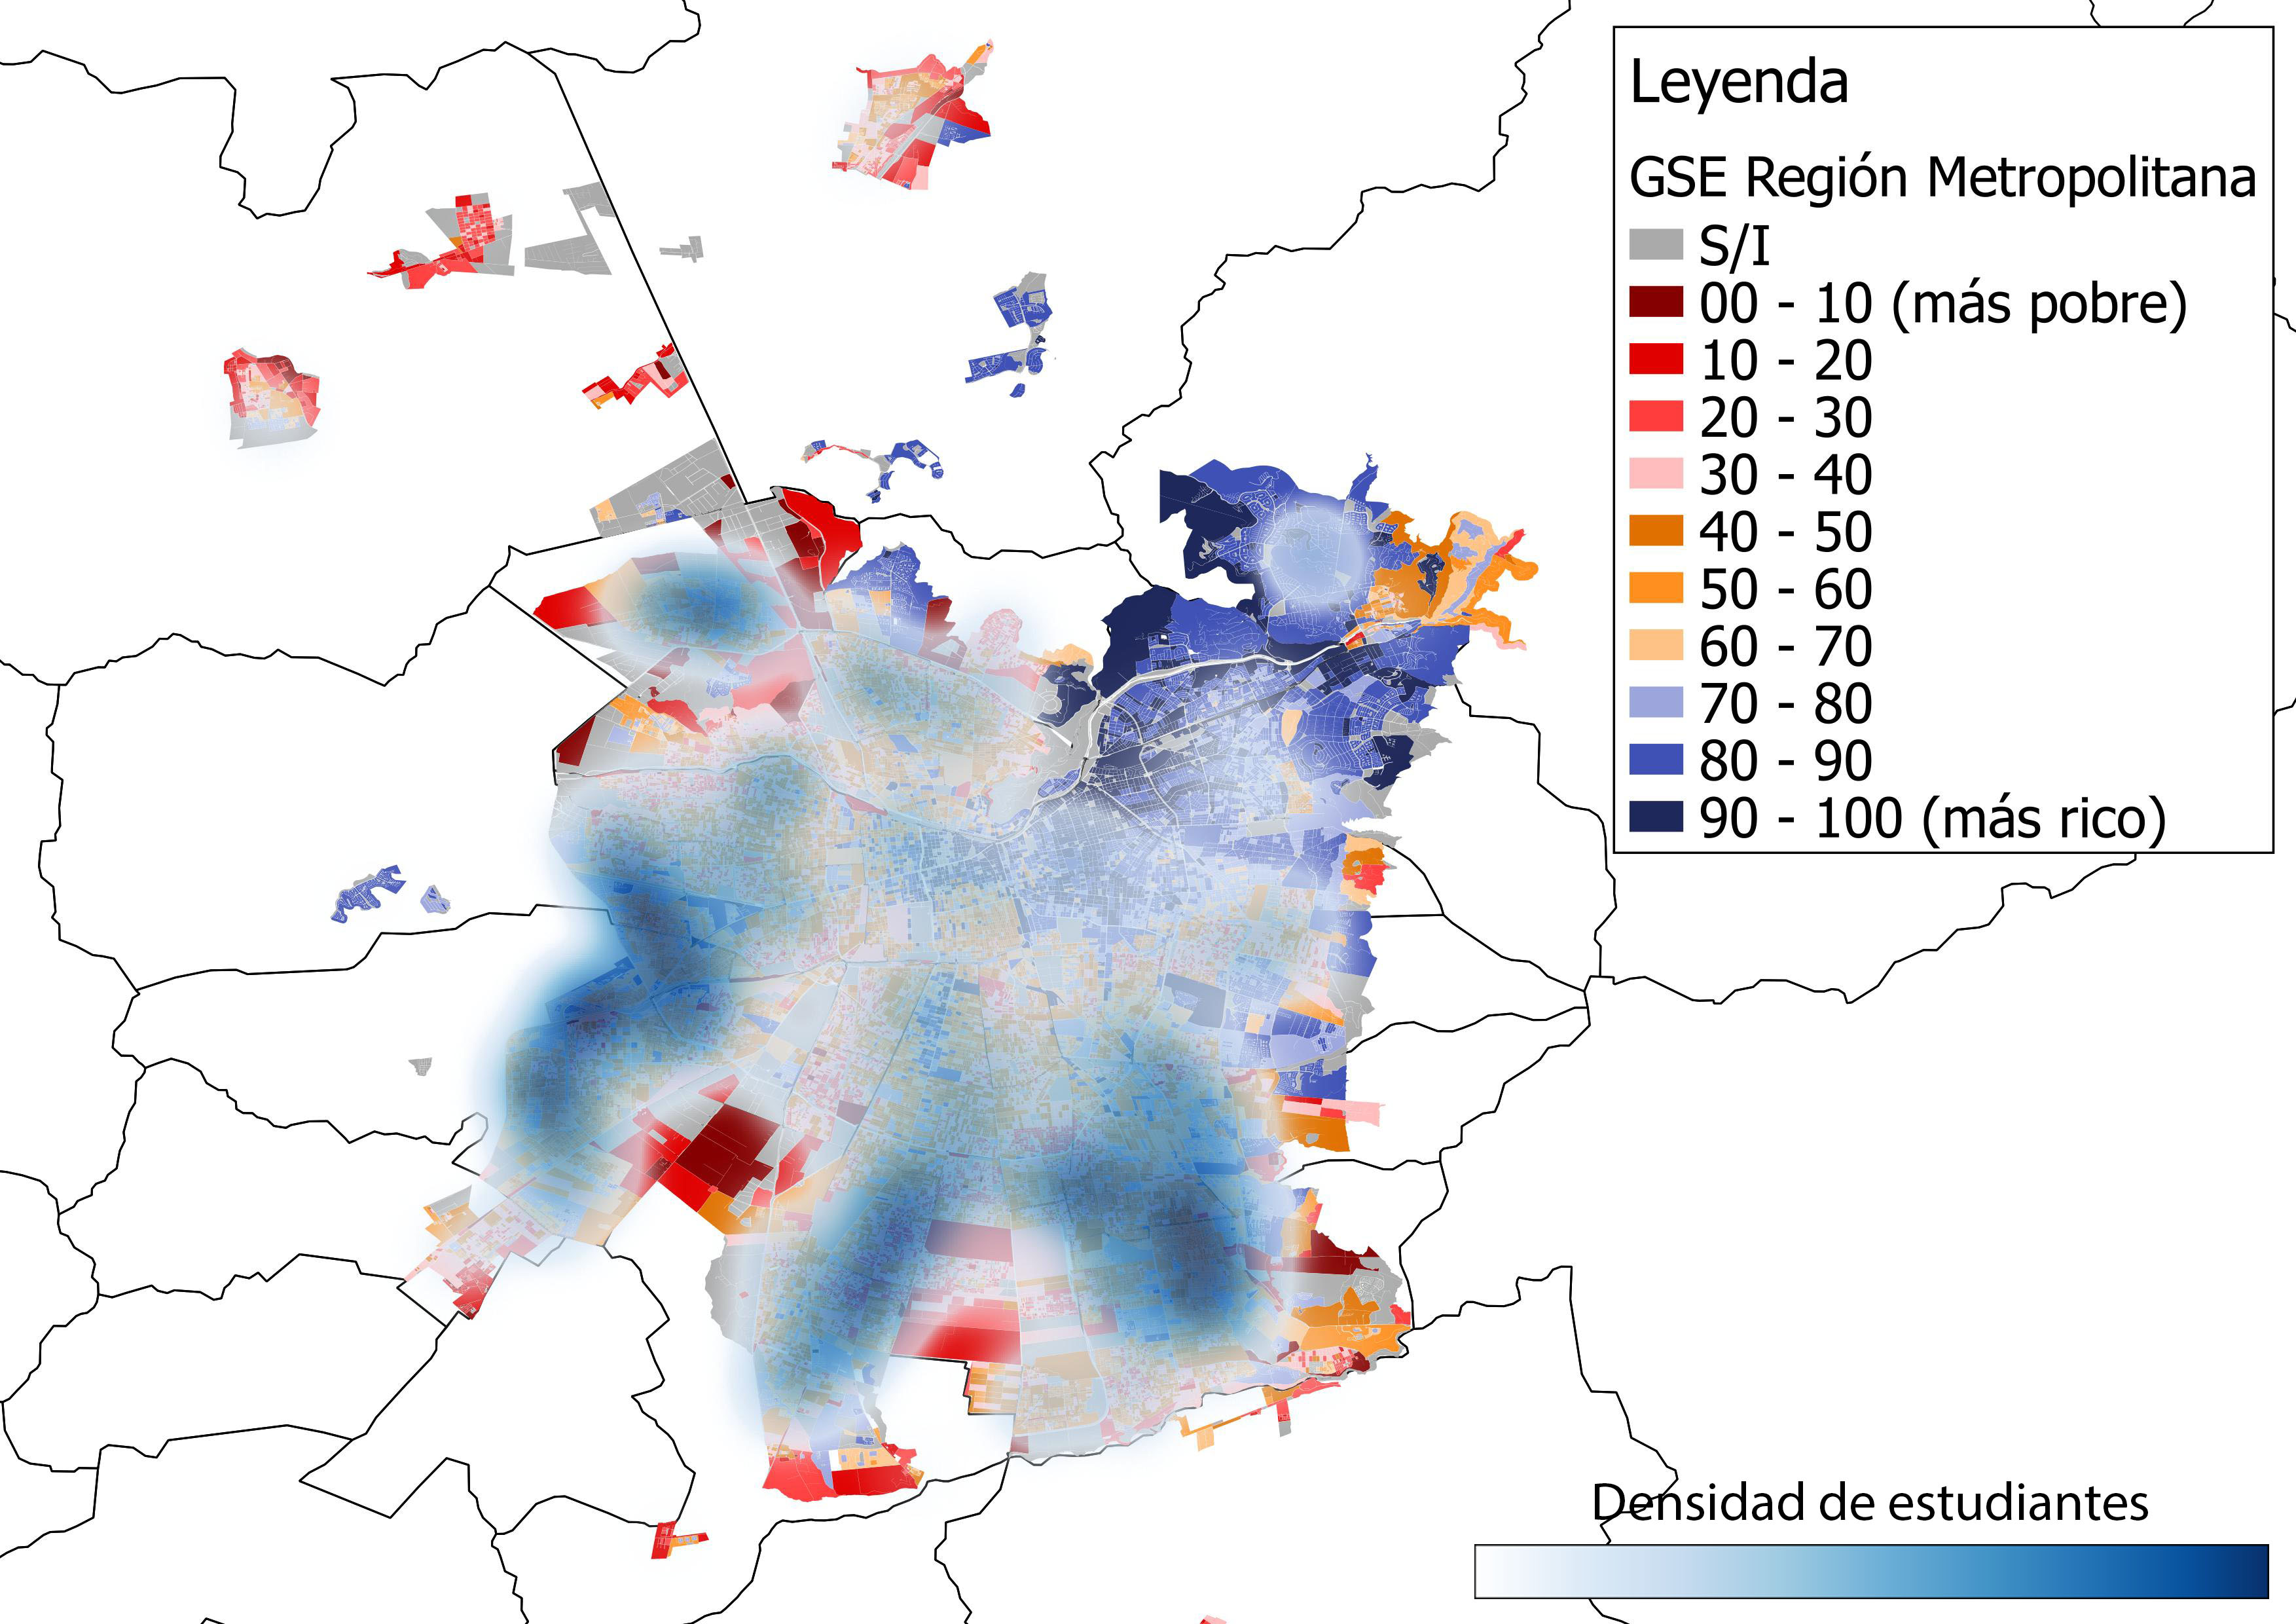
\includegraphics[width=7.5cm]{images/matriculas/M_CON_2_final.jpg}}
  \subfloat[Matrículas clúster MiSBAC.]{
   \label{f:mapa_mat_con_3_gse}
    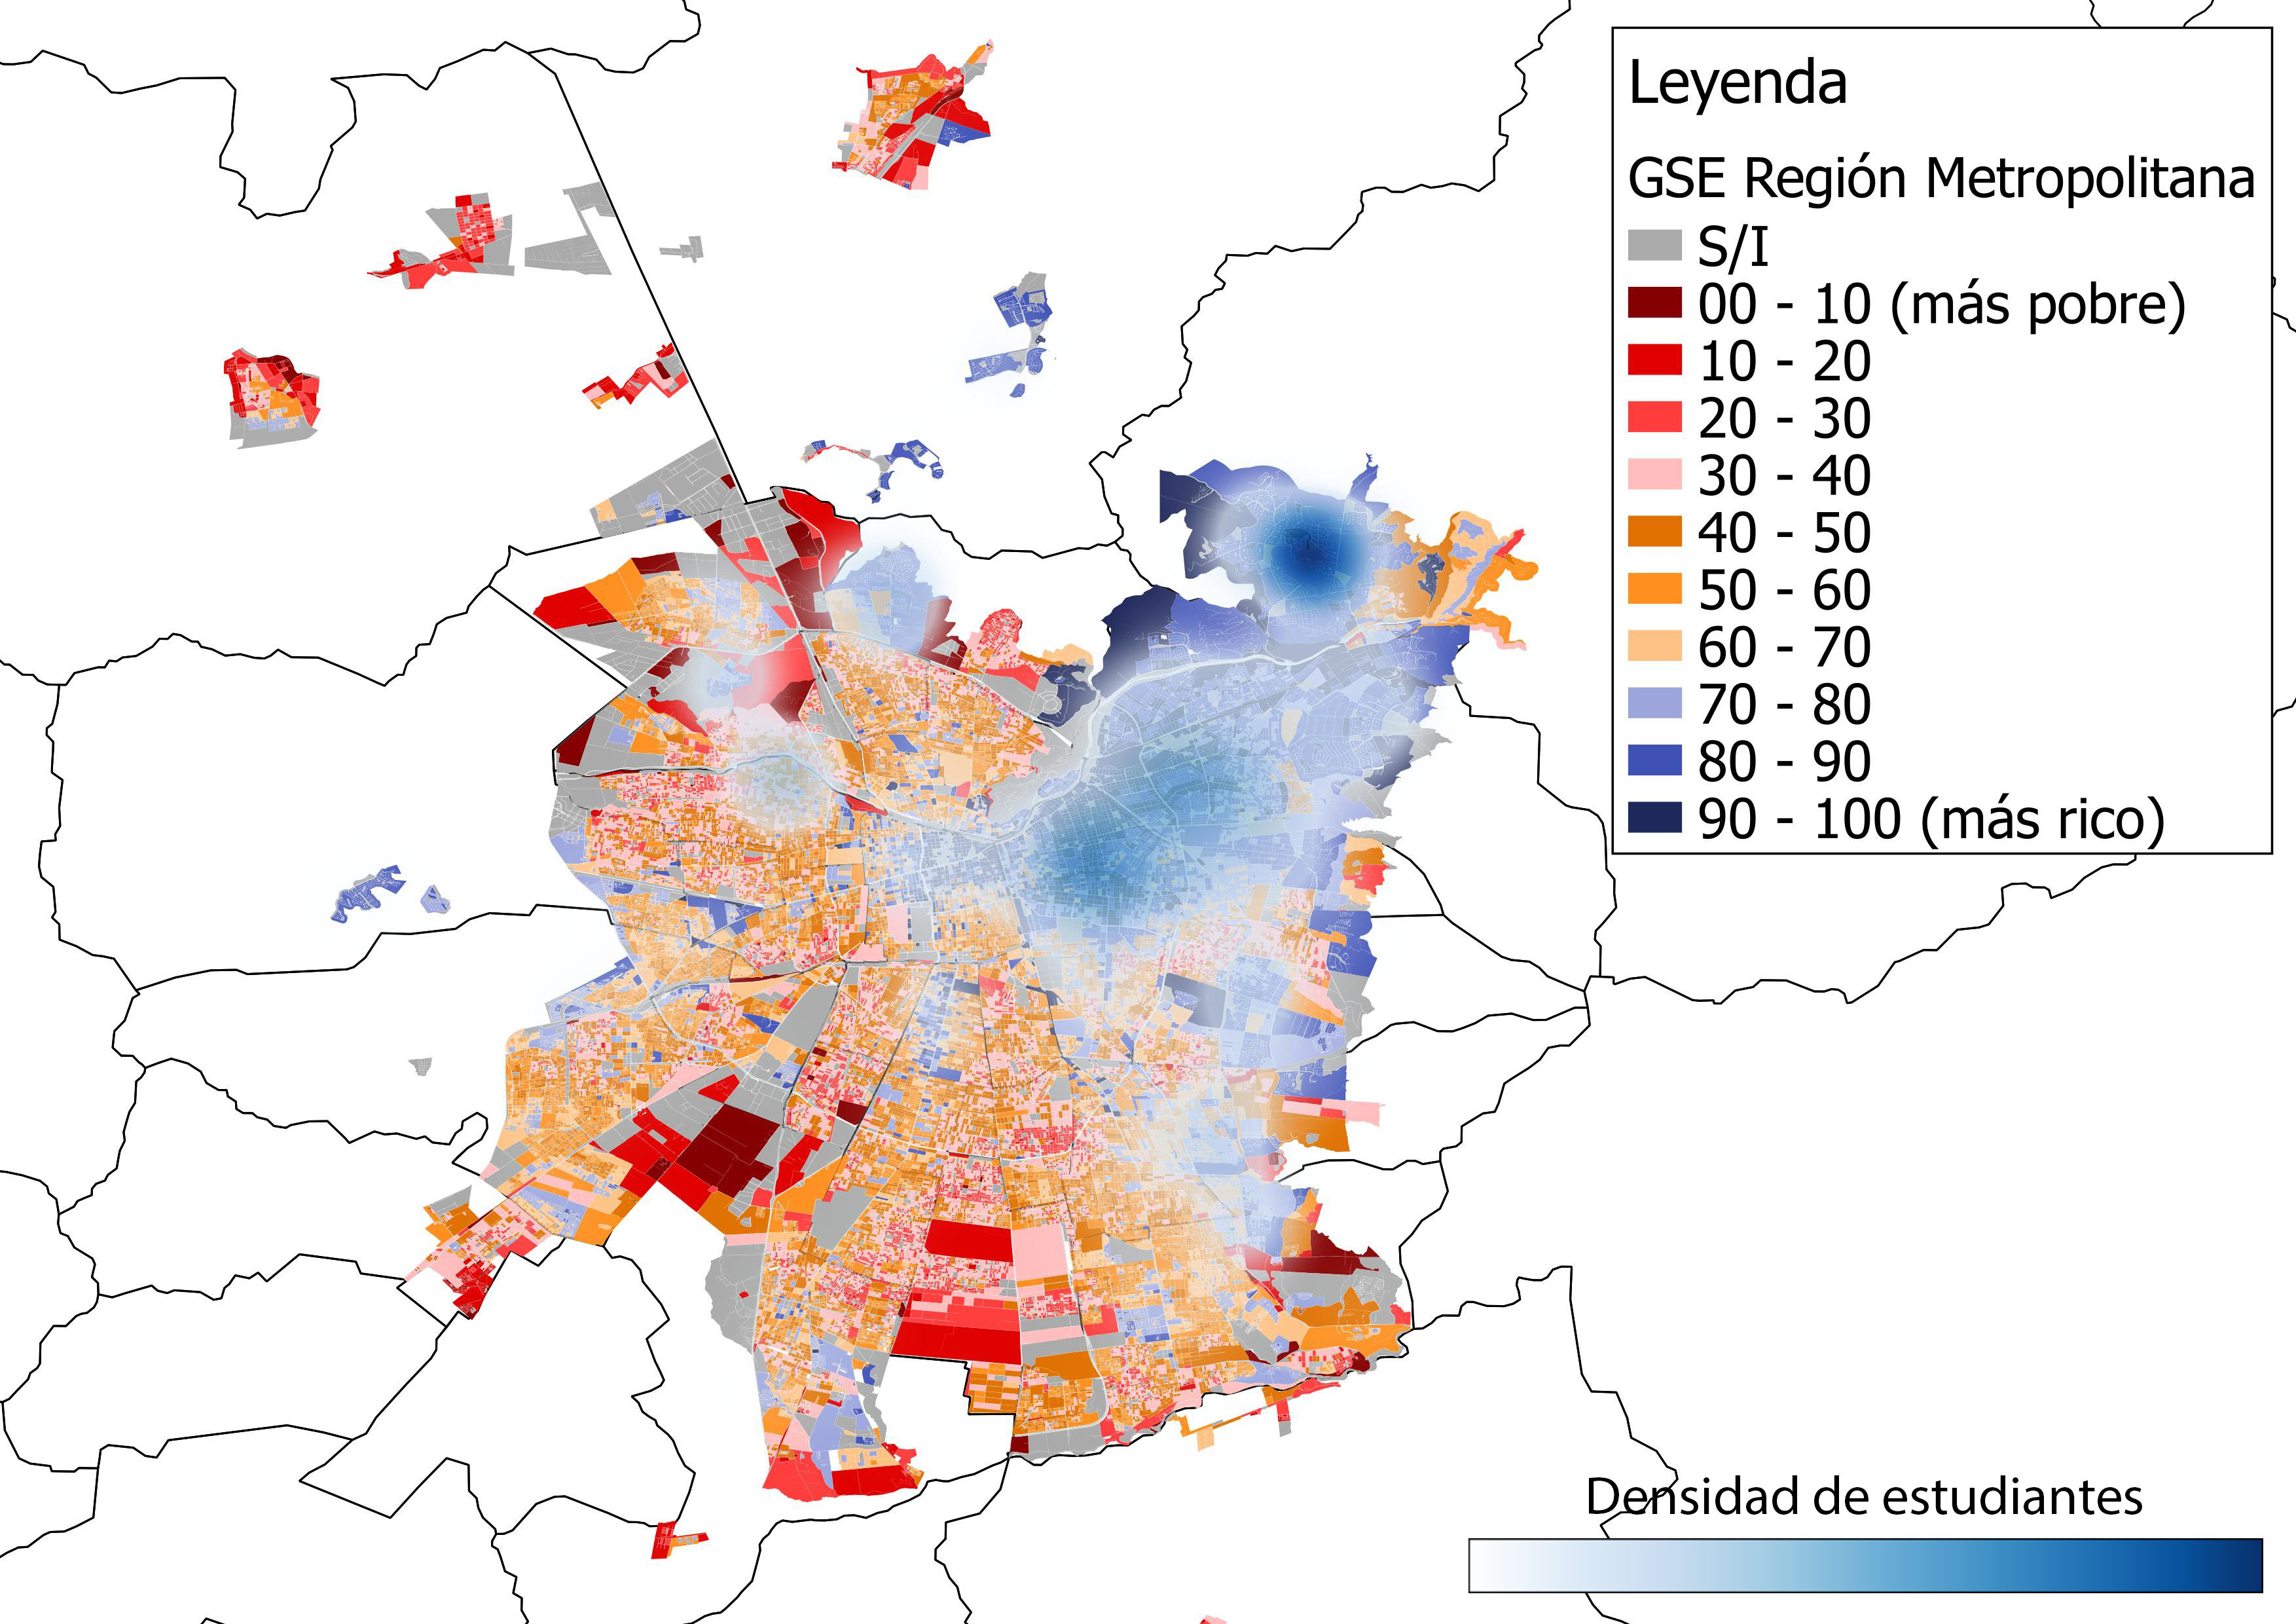
\includegraphics[width=7.5cm]{images/matriculas/M_CON_3_final.jpg}}
 \caption{Mapas de calor de clústers de matrículas (con atributos relacionales) sobre mapa GSE de la Región Metropolitana.}
 \label{f:mapas_mat_con_gse}
\end{figure}